%%% Fiktivní kapitola s instrukcemi k PDF/A

\chapter{Implementácia aplikácie}

Vývoj samotnej aplikácie je rozdelený do dvoch častí backend a frontend. V tejto kapitole si ukáźeme technológie zvolené pre vývoj,
navrhneme a vysvetlíme jednotlivé SPARQL dotazy, ktoré bude backend posielať na Wikidata, popíšeme implementáciu aplikácie a popíšeme implementáciu databázy. 

\section{Technológie použite pre vývoj}

\subsection{Backend}

\subsection*{Voľba jazyka a frameworku }

Backend je možné vyvíjať v rôznych jazykov, kde pre každý jeden z nich existujú frameworky vhodné na vývoj. Pred začiatkom návrhu a implementácie je potrebné zvoliť vhodný jazyk na základe 
dopytu a popularity programovacieho jazyka, alebo podľa požiadavkou potrebných pre vývoj aplikácie. Časte programovacie jazyky pre vývoj backendu sú napríklad Javascript, Python, PHP, Java, alebo Ruby. 
Pre vývoj backendu sme zvolili programovací jazyk Python. Výhoda tohto jazyka je jeho jednoduchosť a to, že existuje obrovské množstvo knižníc pre tento jazyk. 
Podľa mňa je jazyk Python jednoduchý na používanie a kód je ľahko čitateľný. 

Frameworkov pre vývoj backendu v programovacom jazyku Python existuje viacero. Najpopulárnejšie sú asi najskôr Django a Flask. Z týchto dvoch sme zvolili Flask, pretože 
je jednoduchý na používanie, obsahuje málo požiadavkou na iné knižnice a umožňuje vyber preferovaných návrhových vzorov a voľbu databázy. 

\subsection*{Použité knižnice}

Python obsahuje obrovskú štandardnú knižnicu s množstvom modulov, ktoré sú požívané v tejto práci. Tieto moduly si popisovať nebudeme. 

Ako sme už spomínali, hlavnou použitou knižnicou je Flask. Vďaka nemu vytvoríme webový server, s ktorým bude frondend komunikovať pomocou HTTP požiadavkou. 
Jednou z hlavných úloh serveru je na základe parametrov prichádzajúcich na server pomocou HTTP požiadavkou zakonštruovať SPARQL dotazy a tie následne poslať na koncový uzol. Odoslanie SPARQL dotazov a spracovanie vrátených dá 
ma na starosť knižnica SPARQLWrapper, ktorú na túto funkcionalitu použijeme. 

\subsection*{Virtuálne prostredie }

Pre vývoj našej aplikácie použijeme virtuálne prostredie na spravovanie závislosti. To nám vyrieši problém s používaním rôznych verzii knižníc, aby nainštalované balíky pre jeden projekt 
neovplyvňovali ostatné projekty. Python obsahuje modul venv, ktorý slúži na vytváranie virtuálnych prostredí. 

\subsection{Frontend}

\subsection*{Framework a jazyk }
Ako už bolo spomenuté v návrhu architektúry aplikácie, frontend implementujeme ako Single-page aplikáciu. To znamená, že budeme dynamicky prepisovať webovú stránku na základe získaných dát 
z backendu namiesto toho aby sme načítavali úplne nove webové stránky. Pre takýto vývoj aplikácii existuje viacero framworkov a knižníc. 
Zvolili sme Javascriptovú knižnicu React. 
Základom Reactu je stavanie užívateľských rozhraní pomocou takzvaných “komponentov”. Tieto komponenty sú typický napísane použitím JSX (JavaScript Syntax Extension). JSX pripomína jazyk HTML zmiešaní s Javascriptom a z toho 
dôvodu je implementácia komponent jednoduchšia pre developerov poznajúcich HTML. Komponenty môžu byť, ale implementovane čisto použitím Javasciptu bez použitia JSX. V našej implementácii využijeme JSX. 

Javascript nie je typovaný jazyk a z toho dôvodu použijeme Typescript. Ten sa za behu preloží do Javasciptu, ale počas vývoju nám poskytne typovanie premenných. To nám pomôže aby sme sa 
vyhli častým chybám s dynamickými jazykmi ako Javascript. 

\subsection*{Bootstrap}
Aplikáciu v podobe webovej stránky je potrebné vhodne nadizajnovať, aby jednotlivé elementy vyzerali používateľsky rozumne.  Klasický spôsob je použitím jazyka CSS. Počas vývoja aplikácie sa budeme skôr sústrediť na funkcionalitu ako na výzor stránky. Z toho 
dôvodu a ďalších ako napríklad ušetrenie si práce, sme sa rozhodli pre požitie nástroja Bootstrap. Jedná sa o nastroj, ktorý pridáva preddefinovaný výzor elementom na webových stránkach. 
Jedná sa o náhradu CSS. Vďaka Bootstrapu nám stačí vhodne pomenovať triedu elementu a daný element sa už zobrazí tak ako ho Bootstrap preddefinoval. 

\subsection*{Použité knižnice}

Na vývoj frontendu použijeme viacero knižníc. Všetky si uvádzať nebudeme, iba tie najdôležitejšie. Pre možnosť aby bola aplikácia vhodne responzivna použijeme knižnicu react-responsive, ktorá nám pomôže 
pri vyváraní aplikácie. Ako už bolo spomenuté v návrhu, pre implementáciu interaktívnej svetovej mapy využijeme javascriptovú knižnicu Leaflet. 
Zároveň použijeme knižnicu React Leaflet, ktorá poskytuje väzbu medzi knižnicou Leaflet a samotným Reactom. Tato knižnica využíva Leatflet k tomu aby vyjadrila vrstvy Leatfletu ako komponenty Reactu. 



\section{Implementácia SPARQL dotazov}
V tejto sekcii si postupne prejdeme a popíšeme všetky SPARQL dotazy, ktoré naša aplikácia
bude posielať na Wikidata WDQS SPARQL koncový uzol. Pre každý dotaz uvedieme jeho účel, navrhneme a implementujeme
riešenie a popíšeme problémy, ktoré je potrebné počas návrhu a implementácie dotazov riešiť. Jedná sa hlavne
problémy spojené s optimalizáciou, pretože niektoré dotazy trvajú príliš dlho alebo ani neskončia do 60 sekúnd.
V takom prípade  WDSQ presuší proces dotazu a vráti chybu.

\subsection{Vyhľadávanie mapových objektov}

Funkčná požiadavka : Používateľ je schopný vyhľadať konkrétny mapový objekt podľa zadania názvu objektu,
pretože si ho môže chcieť uložiť do svojej kolekcie.

Jedným z prvých a základných dotaz je vyhľadávanie mapových objektov.
Používateľ zadá kľúčový textový reťazec reprezentujúci celý alebo časť názvu mapového objektu.
Podľa poskytnutého reťazca musí aplikácia na strane serveru skonštruovať
SPARQL dotaz, ktorý vyhľadá mapové objekty na základe názvu zhodujúcim sa s textovým reťazcom.

Pre každý nájdený mapový objekt musíme dotazom nielen získať názov, ale aj základne informácie o mapovom objekte potrebne pre aplikáciu.
Zakladám je získať QNumber a názov objektu. Používateľovi je potrebné poskytnúť aj popis objektu aby vedel, čo daný objekt reprezentuje. Z toho
dôvodu musí dotaz pre nájdene objekty získať aj ich popis. Nájdené objekty aplikácia zobrazí používateľovi v podobe zoznamu. Keď používateľ
vyberie niektorý z objektov, ten ktorý hľadal, tak aplikácia zobrazí tento objekt bodom na mape. Pre túto funkcionalitu je potrebne získať
aj súradnice nájdených mapových objektov.

Pri vyhľadávaný podľa názvu je potrebné vyhľadávať iba objekty, ktoré vieme reprezentovať ako mapové objekty v našej aplikácii. Z toho vyplýva, že dotaz musí obsahovať statment, ktorý
z množiny všetkých objektov zhodujúcich sa v názve zahodí tie objekty, ktoré nie sú mapovými objektami.
Riešením je definovať, že množina objektov musí byť inštanciou triedy, ktorá ma nad sebou v hierarchii rozumného rodiča. Tato trieda musí ručiť, že  inštancie všetkých pod-tried tejto triedy sú mapové objekty.
Navrhneme preto triedu "geografická lokácia"(Q2221906). Popis tejto triedy na Wikidatach je nasledovný :
"bod alebo územie na povrchu Zeme alebo aj inde". Tato trieda dobre definuje mapový objekt.

Teraz si ukážme ako by mohol vyzerať dotaz. Najprv sa zaoberajme iba vyhľadávaním objektov na základe názvu a získavanie informácii
o mapovom objekte pridáme až na koniec.

Prvý dotaz, kde vyhľadávame mapové objekty zhodujúce sa s názvom "Tokyo", vyzerá nasledovné:
\begin{code}
      SELECT DISTINCT ?item ?name
      WHERE
      {
      # objekt je "geografická lokácia"
      ?item wdt:P31/wdt:P279* wd:Q2221906.
      # získanie názvu
      ?item rdfs:label ?name.
      # filtrácia, názov objektu iba v anglickom jazyku
      FILTER (lang(?name) = "en")
      # filtrácia, názov objektu musí obsahovať text "Tokyo"
      FILTER(CONTAINS(?name, "Tokyo")).
      SERVICE wikibase:label {
      bd:serviceParam wikibase:language "[AUTO_LANGUAGE],en".
      }
      }
\end{code}

Takýto dotaz ale nezbehne do 60 sekúnd a WDQS ho preruší. Problém je, že WDQS prechádzajú všetky objekty, ktoré
sú v hierarchii inštanciou triedy spadajúcej pod geografickú lokáciu. Následne sa zahadzujú objekty nezhodujúce sa so zadaným názvom.
Objektov "geografická lokácia" existuje obrovské množstvo a WDQS nestihne prejsť za daný čas všetky.

To nie je ale jediný problém. Nahradením triedy "geografická lokácia" za inú triedu napríklad "mesto" vyrieši iba to, že dotaz teraz dobehne, ale
trvá to okolo 15 až 20 sekúnd. Je neprijateľné aby používateľ pri vyhľadávaní objektov podľa zadania názvu musel čakať až 20 sekúnd, kým mu aplikácia vyhľadá objekty.

Tento problém a každý podobný dotaz, kde dochádza k vyhľadávaniu objektov na základe zadania názvu objektu vieme vyriešiť použitím MWAPI.
V MWAPI si zvolíme podporovanú službu "EntitySearch". Tá vyhľadáva Wikibase entity, teda objekty podľa názvu entity, objektu.
Ako vstupne parametre nastavíme jazyk na anglicky. Služba vyhľadáva na základe anglických názvov objektu, a do parametru "search" zadáme textový reťazec poskytnutý používateľom, na základe ktorého bude služba vyhľadávať
objekty. Ako výstupný parameter vyberieme "item", kde do premennej služba priradí všetky nájdené objekty.

Dotaz s použitím služba vyzerá nasledovne:
\begin{code}
      SERVICE wikibase:mwapi {
      # povinný parameter - koncový uzol
      bd:serviceParam wikibase:endpoint "www.wikidata.org";
      # povinný parameter -
      # služba na vyhľadávanie objektov podľa názvu
      wikibase:api "EntitySearch";
      # vyhľadávanie objektov s názvom "tokyo"
      mwapi:search "tokyo";
      # nastavenie anglického jazyka
      mwapi:language "en" .
      # priradenie nájdených objektov do premennej
      ?item wikibase:apiOutputItem mwapi:item.
      ?num wikibase:apiOrdinal true. }
\end{code}

S využitím služby MWAPI dotaz zbehne veľmi rýchlo. Priemer je okolo pol sekundy.
Tým spĺňame nefunkčnú požiadavku:

Aplikácia je dostatočne vykoná. Vyhľadávanie dát na základe zadania názvu v niektorom z vyhľadávačov. Netrvá viac ako sekundu.

Pre kompletný dotaz je potrebné pridať statement, ktorý sa postará aby nájdene objekty boli "geografickými lokáciami" a
pridať trojice na získanie informácií o mapovom objekte. To je názov, opis a súradnice objektu.

Finálny dotaz, pre vyhľadávanie s klúčom "tokyo" vyzerá nasledovne:
\begin{code}
      SELECT DISTINCT
      ?description
      (?lat AS ?lati)
      (?item AS ?QNumber)
      (?lon AS ?long)
      (?itemLabel AS ?name)
      WHERE {
      # služba na vyhľadávanie objektov podľa názvu
      SERVICE wikibase:mwapi {
      bd:serviceParam wikibase:endpoint "www.wikidata.org";
      wikibase:api "EntitySearch";
      mwapi:search "tokyo";
      mwapi:language "en" .
      ?item wikibase:apiOutputItem mwapi:item.
      ?num wikibase:apiOrdinal true. }
      # objekt je "geografickou lokáciou"
      ?item wdt:P31/wdt:P279* wd:Q2221906 .
      # pridanie nápovedi pre optimalizáciu
      hint:Prior hint:gearing "forward".
      # získanie súradníc
      ?item p:P625 ?coord .
      ?coord psv:P625 ?coord_node .
      ?coord_node wikibase:geoLongitude ?lon .
      ?coord_node wikibase:geoLatitude ?lat .
      # získanie opisu
      ?item schema:description ?description .
      # zahodenie opisov, ktoré nie sú v anglickom jazyku
      FILTER (lang(?description) = "en")
      # pridanie služby pre získanie názvov
      SERVICE wikibase:label {
      bd:serviceParam wikibase:language "[AUTO_LANGUAGE],en".
      ?item rdfs:label ?itemLabel .
      }
      # zoradiť výsledky podľa poradia aké boli vrátene MWAPI službou
      } ORDER BY ASC(?num)
\end{code}

Napovedá “hint:Prior hint:gearing "forward"” sa môže použiť za trojicou obsahujúcou cestu.
Je to optimalizačná stratégia, kde povieme dotazu aby prechádzal v opačnom poradí ako je default.
V dotaze rozhodujeme či daný objekt je "geografickou lokáciou".
Default-ne by dotaz začal s triedou "geografická lokácia" a prechádzal rekurzívne jej podtriedy.
My ale použijeme túto stratégiu aby dotaz prechádzal cestu opačne. Začne sa s jednou triedou, ktorou je
objekt inštanciou, a pokračuje sa v prechádzaní jej nad-tried smerom dopredu.

Bez použitia tejto nápovedi je čas dobehnutia dotazu trvá viac ako 1 sekundu a aplikácia teda nesplňuje nefunkčnú požiadavku.

Tento dotaz zároveň použijeme pri vyhľadávaní objektov, ktoré používateľ je schopný definovať ako stred kruhu vo funkčnom požiadavku:
Pre spomínanú definíciu kruhu, v ktorom sa budú objekty vyhľadávať, používateľ je schopný stred tohto kruhu nastaviť na mape posúvaním bodu, alebo
vyhľadaním konkrétneho miesta pomocou vyhľadávania. V takom prípade sa stred kruhu presunie na súradnice nájdeného a vybratého objektu. Pretože používateľ
môže chcieť vyhľadávať objekty v blízkom okolí okolo konkrétneho miesta.

\subsection{Popis a obrázok}
Funkčná požiadavka: Používateľ potrebuje od aplikácie aby mu pre vybraný objekt získala obrázok objektu,
aby používateľ mal predstavu ako objekt vyzerá.

Pre každý uložený mapový objekt, ktorý si používateľ uložil do kolekcie, si v databáze nebudeme udržiavať hodnotu popisu a obrázku objektu.
Je potrebne navrhnúť SPARQL dotaz, ktorý pre zvolený objekt získa obrázok a popis. Tento dotaz sa bude vola, zakaždým keď aplikácia potrebuje prezentovať uložený mapový objekt používateľovi.
Návrh takéhoto dotaz je celkom jednoduchý. Obrázok získame z vlastnosti objektu "obrázok" s identifikačným číslom vlastnosti P18.
Popis na druhú stranu získame použitím prefixu schéma s hodnotou “description” , ktorý získa popis objektu. Popis existuje v rôznych jazykov a preto je ešte potrebne zahodiť v dotaze iné ako ten v anglickom jazyku.

Vlastnosť "obrázok" môže nadobúdať viacero hodnôt, inak povedane existuje viacero obrázkov daného objektu. Pre potreby aplikácie postačí získavať iba jeden z nich.
Tento problém vyriešime použitím agregovanej funkcie SAMPLE. Tá vyberie jeden ľubovoľný obrázok z množiny všetkých obrázkov objektu.
Aby sa dala tato funkcia v dotaze použiť je potrebne zoskupiť výsledky a v tomto prípade je to cez premennú držiacu popis.

Dotaz pre získanie obrázka a popisu pre mesto Tokio (Q1490) vyzerá nasledovne:
\begin{code}
      SELECT
      # vybranie ľubovoľného obrázoku
      (SAMPLE(?img) AS ?image)
      ?desc
      WHERE {
      # získanie obrázka
      wd:Q1490 wdt:P18 ?img .
      # získanie popisu
      wd:Q1490 schema:description ?desc .
      # filtrácia, zahodenie popisov,
      # ktoré nie sú v anglickom jazyku
      FILTER (LANG(?desc) = "en")
      SERVICE wikibase:label {
      bd:serviceParam wikibase:language "[AUTO_LANGUAGE],en".
      }
      # zoskupenie podľa popisu
      } GROUP BY ?desc
\end{code}

\subsection{Odkaz na Wikipédia článok}
Funkčná požiadavka: Používateľ je schopný požiadať aplikáciu aby mu pre vybraný objekt vyhľadala odkaz na článok, sídliaci na Wikipédii, ak článok existuje, aby používateľ mal možnosť
sa o objekte dozvedieť viac informácii vo forme článku.

Aplikácia podporuje iba jeden jazyk a to anglicky. Z toho dôvodu nájdený odkaz na článok o objekte musí sídliť na
anglickej Wikipédií.

Dotaz pre získanie odkazu na článok o objekte na anglickej Wikipédii vyzerá nasledovne:
\begin{code}
      SELECT DISTINCT ?article
      WHERE {
      # získanie článku o objekte
      ?article schema:about wd:Q1490 .
      # článok sídli na anglickej Wikipédií
      ?article schema:isPartOf <https://en.wikipedia.org/> .
      SERVICE wikibase:label {
      bd:serviceParam wikibase:language "[AUTO_LANGUAGE],en".
      }
      }
\end{code}

\subsection{Detaily mapového objektu}
Funkčná požiadavka : Používateľ je schopný požiadať aplikáciu aby mu získala podrobnejšie informácie o objekte(budeme označovať ako detaily objektu), medzi ktorými vie používateľ
filtrovať podľa názvu informácie, aby používateľ získal konkrétnu informáciu o objekte.

Aplikácia získava zdroje jedine z Wikidat pomocou SPARQL dotazov posielajúcich sa na WDQS koncový uzol.
Aplikácia by mohla získavať informácie o mapovom objekte aj z iných zdrojov, ale rozhodli sme sa používať ako zdroj jedine Wikidata.

Na Wikidátach ma každý objekt nejaké vlastnosti obsahujúce jedno alebo viac hodnôt. Každá z týchto vlastnosti poskytuje informáciu o objekte.
Informáciu o objekte označujme ako detail objektu a v tejto pod-sekcii sa zaoberajme ako získavať detaily objektu.

Pôvodný návrh bol statické získavanie detaily. Analyzovali by sme rozumne detaily, spísali ich a vložili do dotazu, ktorý
by bol rovnaký a pre každý mapový objekt by získaval zadané detaily. Každé získavanie vlastnosti by bolo
zabalene do bloku OPTIONAL, pretože nie každú vlastnosť by musel objekt o sebe mať.

Dotaz pre získanie detailov by vyzeral nasledovne:
\begin{code}
      SELECT ?population ?elevation
      WHERE
      {
      OPTIONAL{
                  # Získanie populácie
                  wd:Q1490 wdt:P1082 ?population.
                  # Získanie nadmorskej výšky
                  wd:Q1490 wdt:P2044 ?elevation.
                  # ... ďalšie trojice
                  # pre získanie hodnôt vlastnosti
            }
      SERVICE wikibase:label {
      bd:serviceParam wikibase:language "[AUTO_LANGUAGE],en".
      }
      }
\end{code}

Problém je ale analyzovať rozumne detaily. Možné kategórie mapových objektov existuje obrovské množstvo a objekty v týchto kategóriách môžu obsahovať
zaujímavé detaily, ktoré by sme nezanalyzovali. Je preto potrebne vymyslieť dynamické riešenie.

Ďalší návrh je získavať všetky detaily o objekte. Získať hodnoty všetkých vlastnostiach a tie následne prezentovať používateľovi.
Jedna sa o lepšiu variantu, ale do množiny všetkých detailov pripadnú aj vlastnosti, ktoré nie sú vhodne na prezentovanie používateľovi.
Príkladom môžu byť takzvane "identifikátory". To sú vlastnosti obsahujúce hodnotu ako
identifikátor v inom systéme. Napríklad "OpenStreetMap relation ID", čo je ID relácia daného objektu v OpenStreetMap.
Tento návrh je vhodný na použitie, ale je potrebne vlastnosti rozumne filtrovať.

Každá hodnota vlastnosti je určitého dátové typu. Pri vytváraní novej vlastnosti na Wikidatach sa urči jej
dátový typ a ten sa nemení. Ak ma objekt tuto vlastnosť, tak v nej bude vždy hodnota v tomto dátovom type. Dátový typ vlastnosti zároveň definuje správanie a aké ďalšie dáta môže vlastnosť obsahovať.
Napríklad zoberme si dátový typ "Quantity". Hodnota takéhoto typu vlastnosti môže obsahovať  atribút "unit", ktorý hovorí o v akých jednotkách je kvantitatívna hodnota vyjadrená.
Riešením problému je vymedziť vlastnosti na základe dátového typu.

Exituje viacero dátových typov, ale vymenujme iba tie, ktoré sme po analýze vybrali, že budú podporovane.
Pojmom podporovane myslime, že dotaz bude filtrovať iba tie vlastnosti, ktorých dátový typ patri do množiny vybratých dátových typov.
Vybrane dátové typy sú:
\begin{enumerate}
      \item Monolingualtext - textový reťazec, ktorý nie je preložený do iných jazykov
      \item Quantity - kvantitatívna hodnota reprezentovaná desatinným číslom
      \item Time - dátum vyjadrený v Gregoriánskom alebo Juliánskom kalendári
      \item WikibaseItem - hodnota je iná entita, objekt existujúci na Wikidátach
      \item Url = URL, ktorá identifikuje externý zdroj
\end{enumerate}

Týmto spôsobom vyriešime spomínaný problém s "OpenStreetMap relation ID". Tato vlastnosť nadobúda hodnoty dátového typu
"External identifier", čo je textový reťazec reprezentujúci identifikátor použitý v inom externom systéme.
Keďže v dotaze filtrujeme vlastnosti na základe dátových typov, tak vlastnosti vyjadrene ako External identifier
budú zahodene.

Rozhodnúť v dotaze, či vlastnosť je podporovaného dátové typu dokážeme nasledujúcimi trojicami:
\begin{code}
      # uloženie podporovaných dátových typov do premennej
      VALUES ?supportedDataTypes {
      wikibase:Monolingualtext
      wikibase:Quantity
      wikibase:Time
      wikibase:WikibaseItem
      wikibase:Url  }
      # zahodenie vlastnosti dátového typu, ktorý nie je podporovaní
      ?wd wikibase:propertyType ?supportedDataTypes .
\end{code}
Poznámka: v premennej ?wd sú uložene vlastnosti.

Vlastnosť môže nadobúdať viacero hodnôt. Tieto hodnoty sú označene "rankom".
V dotaze preto zadáme, aby vrátený výsledok dotazu obsahoval pre vlastnosti hodnoty s najlepším, najvhodnejším rankom. To spravíme nasledovne:
\begin{code}
      # získanie hodnoty s najlepším rankom
      ?statement rdf:type wikibase:BestRank .
\end{code}

Po analýze tohto dotazu sme ale našli zopár vlastnosti s podporovaným dátovým typom, ktoré nie sú v kontexte detailov vhodne.
Napríklad vlastnosť "je inštanciou" (P131). Hodnotu tejto vlastnosti získavame v inom dotaze a následne ju
ukladáme do databázy s mapovým objektom. Tieto hodnoty definujú mapový objekt a často krát ich aplikácii prezentuje používateľovi.
Preto je vhodné si tento údaj uložiť do databázy. Z toho dôvodu tuto vlastnosť nie je potrebné znovu získavať v kontexte získavania detailov.

Nežiadúce vlastnosti definujeme ako zoznam a v dotaze ich vyfiltrujeme nasledovne:
\begin{code}
      FILTER (?wd not in ( wd:P190 , wd:P31 , wd:P150 , wd:P355 , wd:P131 , wd:P1383 ))
\end{code}
Poznamka: v premennej ?wd sú uložené vlastnosti.

Posledným problém je, že hodnoty niektorých dátových typov obsahujú ďalšie doležíte informácie.
Konkrétne dátový typ "Time" obsahuje "timePrecision", v ktorej je vyjadrená precíznosť času. To znamená, či
dátum ako hodnota v tejto vlastnosti ma byť interpretovaná ako cely dátum, rok alebo storočie. Tato informácia je potrebná pre
interpretovanie a zobrazovanie časového detailu používateľovi.

Pre vlastnosti s dátovým typom "Quantity" je potrebné získať informáciu v "quantityUnit", ktorá obsahuje
jednotku v ktorej je kvantitatívna hodnota vyjadrená.

Tieto informácie sú pre aplikáciu nevyhnutné aby dokázala správne prezentovať detaily.

Aby sme nemuseli pre tieto dátové typy vytvárať rozdielne dotazy, tak získavanie týchto dvoch informácii obalíme do
OPTIONAL bloku.

Kompletný dotaz vyzerá nasledovne:
\begin{code}
      SELECT DISTINCT
      ?unit
      ?property
      (GROUP_CONCAT( DISTINCT ?valueLabel ;separator="<space>") AS ?values)
      ?dataType
      ?timePrecision
      WHERE {
      # získanie všetkých vlastnosti
      wd:Q1490 ?p ?statement .
      # získanie hodnôt s najlepším rankom
      ?statement rdf:type wikibase:BestRank .
      ?statement ?ps ?ps_ .
      ?wd wikibase:claim ?p .
      ?wd wikibase:statementProperty ?ps .
      ?wd wikibase:statementValue ?psv .
      # definovanie podporovaných dátových typov
      VALUES ?supportedDataTypes {
      wikibase:Monolingualtext
      wikibase:Quantity
      wikibase:Time
      wikibase:WikibaseItem
      wikibase:Url  }
      # zahodenie vlastnosti s iným dátovým typom
      ?wd wikibase:propertyType ?supportedDataTypes .
      # zahodenie konkrétnych nežiadúcich vlastnosti
      FILTER (?wd not in ( wd:P190 , wd:P31 , wd:P150 , wd:P355 , wd:P131 , wd:P1383 ))
      # získanie dátového typu
      ?wd wikibase:propertyType ?dataType .
      # získanie hodnoty vlastnosti
      ?statement ?ps ?value .
      # získanie časovej precíznosti
      # ak je vlastnosť dátového typu "Time"
      OPTIONAL {?statement ?psv [wikibase:timePrecision  ?timePrecision].}
      # získanie jednotky
      # ak je vlastnosť dátového typu "Quantity"
      OPTIONAL {?statement ?psv [wikibase:quantityUnit  ?unitValue].}
      SERVICE wikibase:label {
      bd:serviceParam wikibase:language "[AUTO_LANGUAGE],en".
      ?wd rdfs:label ?property .
      ?value rdfs:label ?valueLabel.
      ?unitValue rdfs:label ?unit. }
      } GROUP BY ?dataType ?timePrecision ?property ?unit
\end{code}

Ak vlastnosť nadobúda viacero hodnôt, tak tieto hodnoty zoskupíme do jednej hodnoty obsahujúcu
decimeter aby následne vedela aplikácia rozdeliť a interpretovať samotné hodnoty. Z toho dôvodu zoskupíme vlastnosti a použijeme
agregovanú funkciu GROUP CONCAT.

\subsection{Vyhľadávanie kategórii}
Funkčná požiadavka:  Používateľ potrebuje od aplikácie možnosť vyhľadať možne a rozumné triedy definujúce
objekty podlá názvu triedy, aby sa následne trieda dala použiť ako parameter.

Počas vyhľadávania skupiny mapových objektov používateľ môže zadať parametre, ktoré ovplyvnia nájdenú skupinu mapových objektov. Prvým týmto parametrom je výber kategórie. Kategória je vyjadrená ako
trieda na Wikidatach definujúca určitú skupinu objektov.
Používateľ potrebuje vyhľadať a následne vybrať kategóriu na základe názvu. Navrhneme preto dotaz vyhľadávací rozumne triedy, ktoré
je možne použiť ako kategóriu v aplikácii.
Vyhľadávanie na základe názvu je rovnaké ako u vyhľadaní mapovych objektov. Použijeme MWAPI službu “EntitySearch”.
Zároveň získame názov a popis triedy aby používateľ bol schopný lepšie pochopiť danú triedu, aký skupinu objektov reprezentuje. QNumber získame
aby aplikácia vedela neskôr použiť tuto kategórii v dotaze pre vyhľadávanie skupiny objektov ako parameter definujúci kategóriu.

Nájdene výsledky musia byť vhodne triedy. Po analýze hierarchie Wikidát navrhneme, že vhodné triedy musia patriť v hierarchii pod triedou "geografická lokácia" (Q2221906).

Dotaz vychládajúci vhodné kategórie s kľúčovou hodnotou "jaskyne" vyzerá nasledovné:
\begin{code}
      SELECT DISTINCT
      (?item AS ?QNumber)
      ?description
      (?itemLabel AS ?name)
      WHERE {
      # vyhľadanie objektov na základe názvu
      SERVICE wikibase:mwapi {
      bd:serviceParam wikibase:endpoint "www.wikidata.org";
      wikibase:api "EntitySearch";
      mwapi:search "castle";
      mwapi:language "en" .
      ?item wikibase:apiOutputItem mwapi:item.
      ?num wikibase:apiOrdinal true. }
      # priradenie hodnôt do premenenej
      VALUES ?classRestrictions {wd:Q2221906  }
      # objekt musí spadať pod triedu
      # geografická lokácia
      ?item wdt:P279* ?classRestrictions .
      # napovedá na optimalizáciu
      hint:Prior hint:gearing "forward".
      # získanie popisu objektu
      ?item schema:description ?description .
      # zahodenie iných popisov ako tie v anglickom jazyku
      FILTER (lang(?description) = "en")
      SERVICE wikibase:label {
      bd:serviceParam wikibase:language "[AUTO_LANGUAGE],en".
      ?item rdfs:label ?itemLabel . }
      } ORDER BY ASC(?num)
\end{code}

Od aplikácie očakávame možnosť definovať aj výnimky. Tieto výnimky sú triedy spadajúce pod triedu vybratej kategórie.
Dotaz vychládajúci pod-kategórie je rovnaký ako vyššie uvedený, ale do premennej ?classRestrictions namiesto "geografickej
lokácie" priradíme triedu, ktorá identifikuje vybratú kategóriu.

Keď si používateľ vyberie kategóriu a vyberie aj nejakú pod-kategóriu, a následne chce ďalej vyhľadávať ďalšie možné pod-kategórie, tak
je očakávane, že dotaz zahodí pod-triedy spadajúce pod už zvolené pod-kategórie. Tento problém vyriešime
pridaním MINUS bloku, kde rovnakým princípom, ako sme vyjadrovali, že trieda musí spadať pod triedu "geografická lokácia",
vyriešime zahodenie tých tried, ktoré spadajú pod triedy zvolených pod-kategórií ako výnimky.

Pridaná časť dotazu vyzerá nasledovné:
\begin{code}
      MINUS{
      VALUES ?classExceptionRestrictions {wd:Q3480180  }
      ?item wdt:P279* ?classExceptionRestrictions .
      hint:Prior hint:gearing "forward".
      }
\end{code}
Poznámka: do premennej ?classExceptionRestrictions priradíme triedy, ktoré sú vybraté ako výnimky.

\subsection{Vyhľadávanie administratívneho územia a regiónov}
Funkčná požiadavka: Používateľ je schopný vyhľadať podlá názvu a definovať parameter územia ako súčasne existujúce územie, aby používateľ vedel vyhľadávať objekty
na území kontinentu, krajiny alebo administratívneho územia.

Vyhľadávanie skupiny mapových objektov podporuje definovanie oblasti, respektíve územia, v ktorom sa musia vyskytovať nájdene mapové objekty.
Územie môže byť definované ako cely svet, na ktorý nepotrebujeme dotaz, región , krajina a administratívne územie.
Krajina je administratívne územie, teda spadá nám do dotazu na vyhľadávanie administratívneho územia.

Navrhneme dva rozdielne dotazy. Jeden na vyhľadávanie administratívneho územia a druhy na vyhľadávanie regiónov.

\subsection*{Vyhľadávanie administratívneho územia }
Dotaz na vyhľadávanie administratívneho územia navrhneme rovnakým princípom ako vyhľadávanie kategórii.
Triedu "geografickej lokácie" nahradíme za "administratívny územný celok" (Q56061). Pri vyhľadávaní kategórii bolo
potrebne aby nájdene objekty boli triedy. V tomto dotaze potrebujeme vyhľadávať inštancie, preto musíme pozmeniť predikát
z wdt:P279* na wdt:P31/wdt:P279*, vďaka ktorému dotaz vyhľadá inštancie.

Po analýze Wikidat je ešte potrebné do dotazu pridať výnimky, teda triedy, ktorých nájdene objekty nesmú byť inštanciou.
Sú to "nepolitická administratívna jednotka" (Q15642566) a "historické administratívne územie" (Q19832712), ktoré definuje, že objekt je historické administratívne
územie. Dôvod je časť z funkčného požiadavku: "súčasne existujúce územie".

Rovnako ako u možnosti zvoliť pod-kategórie vybratej kategórii ako výnimku, tak aj u administratívneho územia
aplikácia umožňuje definovať výnimky ako administratívne územia, ktoré spadajú do vybranej administratívnej oblasti.

Do dotazu pridáme trojice, ktoré sa postarajú o to aby nájdene administratívne oblasti, ktoré používateľ vyhľadáva
pre definovanie výnimiek, boli súčasťou vybranej
konkrétnej administrovanej oblasti. Na to poslúži predikát "nachádza sa v administratívnej jednotke" (P131).

Zároveň rovnakým princípom pridáme možnosť zahadzovať tie administratívne územia, ktoré spadajú pod administratívne územia, ktoré
sú vybraté ako výnimky.

Pridaná časť dotazu vyzerá nasledovne:
\begin{code}
      # zahodenie území, ktoré nespadajú pod
      # administratívne územie Q214
      VALUES ?locatedInAreas {wd:Q214  }
      ?item wdt:P131* ?locatedInAreas .
      hint:Prior hint:gearing "forward".
      # zahodenie území, ktoré spadajú pod
      # administratívne územie Q181342
      MINUS{
      VALUES ?notLocatedInAreas {wd:Q181342  }
      ?item wdt:P131* ?notLocatedInAreas .
      hint:Prior hint:gearing "forward".
      }
\end{code}

\subsection*{Vyhľadávanie regiónu }
Dotaz pre vyhľadávanie regiónu začína rovnako použitím MWAPI na vyhľadanie objektov podľa názvu.

Následne musíme v dotaze obmedziť nájdene objekty na to aby boli objektami reprezentujúce región.
Regiónom myslime oblasť do ktorej niektorá krajina patri. Preto navrhneme toto obmedzenie nasledovne.
Zoberieme všetky objekty, ktoré sú inštanciou "nezávislý štát" (Q3624078) a vyjadrime, že
nájdene objekty musia:
\begin{enumerate}
      \item patriť do množiny objektov obsahujúcich územia. Tieto územia získame z vlastnosti "patriť" (P361).
            Objekt reprezentujúci krajinu má vlastnosť "patriť" kde sú ako hodnoty objekty reprezentujúce územie, región, do ktorého daná krajina patri.
      \item objekt je inštanciou "geografický región" (Q82794)
      \item alebo objekt je inštanciou "kontinent" (Q5107).
\end{enumerate}
Na spojenie týchto vyjadrení použijeme UNION blok.

Pri analýze dospejeme k záveru, že dotaz vracia aj objekt "planétu Zem" (Q2). Tento objekt nie je vhodný ako región a preto ho v dotaze
zahodíme.

Dotaz na vyhľadanie regiónov s kľúčom "europe" vyzerá nasledovne:
\begin{code}
      SELECT DISTINCT
      ?description
      (?itemLabel AS ?name)
      (?item AS ?QNumber)
      WHERE {
      # vyhľadanie objektov na základe názvu
      SERVICE wikibase:mwapi {
      bd:serviceParam wikibase:endpoint "www.wikidata.org";
      wikibase:api "EntitySearch";
      mwapi:search "europe";
      mwapi:language "en" .
      ?item wikibase:apiOutputItem mwapi:item.
      ?num wikibase:apiOrdinal true. }
      # získanie nezávislých krajín sveta
      ?country wdt:P31 wd:Q3624078 .
      # obmedzenie
      # objekt je geograficky región
      # a patri do množiny
      # získanej ako hodnoty z vlastnosti
      # "súčasť" všetkých nezávislých krajín
      { ?country wdt:P361 ?item.
      ?item wdt:P31 wd:Q82794.}
      UNION
      # objekt je kontinent
            { ?item wdt:P31 wd:Q5107.}
      # zahodenie objektu "planét Zem"
      FILTER (?item not in (wd:Q2))
      # získanie popisu regiónu
      ?item schema:description ?description .
      # zahodenie popisov, ktoré nie sú
      # v anglickom jazyku
      FILTER (lang(?description) = "en")
      SERVICE wikibase:label {
      bd:serviceParam wikibase:language "[AUTO_LANGUAGE],en".
      ?item rdfs:label ?itemLabel . }
      } ORDER BY ASC(?num)
\end{code}


\subsection{Vlastnosti ako filtre }
Funkčná požiadavka: Používateľ je schopný v procese vyhľadávania objektov definovať nejaké vlastnosti objektu, ktoré musia nájdene objekty splňovať, aby používateľ mohol zadať vlastnosti,
ktoré očakáva, že nájdené objekty budú splňovať.

V procese vyhľadávania skupiny objektov od aplikácie je očakávaná možnosť ako parameter definovať vlastnosti s hodnotou, ktoré musia hľadané objekty splňovať.

Každá vlastnosť je nejakého dátové typu a ku každému dátovému typu sa viažu obmedzenia. V návrhu podporujeme iba vlastnosti troch dátových typov. Sú to Quantity, Time a WikibaseItem.

\subsection*{Vyber možných vlastnosti }

Prvý návrh bol aby aplikácia podporovala možnosť vybrať ako filter iba z množiny zopár vlastnosti, ktoré zanalyzujeme a pridáme do dotazu pre vyhľadávanie skupiny objektov.
Tento návrh nie je prakticky a preto sme prišli s dynamickým návrhom.
Navrhneme dotaz, ktorý pre konkrétnu kategóriu získa zoznam vlastnosti. Vlastnosti v zozname dávajú zmysel pre konkrétnu kategóriu.
Napríklad vlastnosť "populácia" sa viaže ku kategórii ako mesto alebo krajina a nie ku hradom. Zoznam nazveme ako "odporúčane vlastnosti" pre danú zvolenú kategóriu.

V tomto probléme nám dosť pomôže vlastnosť "vlastnosti tohto typu"(P1963).
Trieda reprezentujúca kategóriu môže mať tuto konkrétnu vlastnosť. V nej nájdeme zoznam vlastnosti, ktoré sa často spájajú s danou triedou.
Urobíme to ale rekurzívne. Zoberieme konkrétnu kategóriu, respektíve triedu, ktorú si používateľ vybral a prejdeme všetky nad-triedy tejto triedy rekurzívne.
Pre každú prechádzanú triedu skúsime zistiť ci ma vlastnosť P1963 obsahujúcu vlastnosti, ktoré si uložíme do premennej. Nebudeme však prechádzať všetky triedy.
Do úvahy zoberieme iba triedy, ktoré v hierarchii spadajú pod triedu "geografická lokalita". Vďaka tomu dostaneme iba vlastnosti, ktoré sa logicky spájajú ku
geografickým lokalitám, čo sú naše kategórie.

V dotaze ešte zahodíme vlastnosti "krajina"(P17) a “nachádza sa v administratívnej jednotke" (P131), pretože tieto vlastnosti používateľ definuje parametrom vyber oblasti, kde
sa musia nájdene mapové objekty vyskytovať.

Na koniec je ešte potrebne zahodiť vlastnosti , ktoré nie sú podporovaného dátového typu.

Pre každú vlastnosť získame názov, PNumber ako identifikáciu vlastnosti na použitie v iných dotazov,
popis, aby používateľ vedel, čo daná vlastnosť reprezentuje, a dátový typ vlastnosti.

Dotaz na získanie odporúčaných vlastnosti kategórie "hrady" vyzerá nasledovne:
\begin{code}
      SELECT DISTINCT
      ?description
      (?property AS ?PNumber)
      (?propertyLabel AS ?name)
      ?dataType
      WHERE {
      # získanie všetkých nad-tried triedy hrad
      wd:Q23413 wdt:P279* ?classes .
      # triedy musia byt pod-triedou "geografická lokácia"
      VALUES ?superClasses {wd:Q2221906  }
      ?classes wdt:P279* ?superClasses .
      hint:Prior hint:gearing "forward".
      # získanie všetkých vlastnosti
      # ktoré sa viažu k nejakej z tried
      ?classes wdt:P1963 ?property .
      # zahodenie konkrétnych tried
      FILTER (?property not in ( wd:P131 , wd:P17 ))
      # zahodenie vlastnosti, ktoré
      # nie sú podporovaného dátového typu
      VALUES ?supportedDataTypes {
      wikibase:Time
      wikibase:Quantity
      wikibase:WikibaseItem  }
      ?property wikibase:propertyType ?supportedDataTypes .
      # získanie dátového typu
      ?property wikibase:propertyType ?dataType .
      # získanie popisu
      ?property schema:description ?description .
      FILTER (lang(?description) = "en")
      SERVICE wikibase:label {
      bd:serviceParam wikibase:language "[AUTO_LANGUAGE],en".
      ?property rdfs:label ?propertyLabel . }
      }
\end{code}

Problém ale je, že niektoré vlastnosti nedostaneme pre danú kategórie ako odporúčanú vlastnosť. Napríklad pre kategóriu hrad
nedostaneme vlastnosť "pamiatkový status" (P1435), ktorou vieme vyhľadávať hrady patriace k UNESCO pamiatkam.

Musíme preto umožniť používateľovi zvoliť danú vlastnosť nielen zo zoznamu odporúčaných filtrov ale aj zo zoznamu, ktorý označíme ako
"všetky vlastnosti". Tento zoznam samozrejme neobsahuje úplne všetky existujúce vlastnosti na Wikidatach.

Zoberme všetky triedy spadajúce pod triedu "geografická lokalita".
Pre každú z tried priradíme všetky hodnoty z vlastnosti "vlastnosti tohto typu"(P1963)
do premennej. Nasleduje rovnaký postup ako pri "odporúčaných filtrov".
V zozname "všetky vlastnosti" nájdeme už aj napríklad vlastnosť "pamiatkový status".

Tento dotaz je ale veľmi nároční. Trvá veľmi dlho kým skonči, dokonca ak je WDQS zaťažene nemusí nedobehnúť do stanoveného limitu.
Keďže ale tento zoznam je rovnaký pre každú zvolenú kategóriu, tak výsledok tohoto dotazu si uložíme na server
a keď aplikácia požiada server o tento zoznam, tak server vráti rovno výsledok z uloženého súboru.

\subsection{Obmedzenia vlastnosti }
Každá vlastnosť obsahuje svoje špecifické obmedzenia, ktoré je potrebné získať aby aplikácia umožnila
používateľovi zadávať validnú hodnotu vlastnosti. Tieto obmedzenia sú vyjadrene ako hodnoty vlastnosti "obmedzenie" (P2302) a sú
nevyhnutné pre správne vyhľadávanie a zadávanie hodnôt.
Obmedzenia sú zároveň pre každý dátový typ rozdielne. Preto je potrebné získavať rozdielne obmedzenia na základe dátového typy.

Aplikácia podporuje tri dátové typy.

\begin{enumerate}
      \item Time - pre tento dátový typ nie je potrebne získavať obmedzenia, pretože používateľ zadáva dátum
      \item Quantity - používateľ zadáva desatinne číslo a preto je potrebne získať povolený rozsah tohto čísla,
            teda minimálnu a maximálnu povolenú hodnotu čísla. Číslo môže byt vyjadrene používateľom v rôznych jednotkách.
            Z toho dôvodu je potrebné získať zoznam povolených jednotiek, ktorými môže byt desatinne číslo vyjadrene v konkrétnej vlastnosti.
      \item WikibaseItem - používateľ ako hodnotu zadá iný objekt z Wikidat, ten ale musí si vyhľadať podľa názvu. V tomto vyhľadávaní
            nechceme umožniť vyhľadávať všetky objekty. Je vhodné vyhľadávať iba tie, ktoré môžu byt použite ako hodnota pre tuto vlastnosť. Pre to je potrebne
            získať z obmedzení informácie o obmedzeniach definujúce množinu objektov.
\end{enumerate}

\subsection*{Quantity obmedzenia }
Pre kvantitatívne vlastnosti aplikácia potrebuje dva dotazy na obmedzenia. Jeden pre získanie obmedzení reprezentujúce maximálnu a minimálnu povolenú hodnotu
a druhy pre získanie zoznamu povolených jednotiek.

Maximum a minimum, danej hodnoty vlastnosti, sú
vyjadrene ako kvantifikátory "minimum value" (P2313)
a "maximum value" (P2312) v hodnote "range constraint" (Q21510860).

Dotaz pre získanie rozsahu pre vlastnosť "nadmorská výška" (P2044) vyzerá nasledovne:
\begin{code}
      SELECT  ?min ?max
      WHERE {
      # získanie uzlu
      # daný uzol bude použitý ako predmet
      wd:P2044 p:P2302 ?node .
      # získanie objektu obsahujúci povolený rozsah
      ?node ps:P2302 wd:Q21510860 .
      # získanie hodnoty kvantifikátoru minimálna hodnota
      ?node pq:P2313 ?min .
      # získanie hodnoty kvantifikátoru maximálna hodnota
      ?node pq:P2312 ?max .
      SERVICE wikibase:label {
      bd:serviceParam wikibase:language "[AUTO_LANGUAGE],en".
      }
      }
\end{code}

Zoznam povolených jednotiek nájdeme ako hodnoty v kvantifikátore "item of property constraint" (P2305)
v hodnote "allowed units constraint" (Q21514353).

Dotaz pre získanie povolených jednotiek pre vlastnosť "nadmorská výška" (P2044) vyzerá nasledovne:
\begin{code}
      SELECT  (?item AS ?QNumber) (?itemLabel AS ?name)
      WHERE {
      # získanie uzlu
      # daný uzol bude použitý ako predmet
      wd:P2044 p:P2302 ?node .
      # získanie objektu obsahujúci povolene jednotky
      ?node ps:P2302 wd:Q21514353 .
      # získanie hodnoty kvantifikátoru
      ?node pq:P2305 ?item .
      SERVICE wikibase:label {
      bd:serviceParam wikibase:language "[AUTO_LANGUAGE],en".
      ?item rdfs:label ?itemLabel .
      }
      }
\end{code}

\subsection*{WikibaseItem obmedzenia}
Pre vlastnosti tohto dátové typu bude aplikácia potrebovať štyri dotazy. V každom jednom z nich získame
iný druh obmedzenia, ktoré obmedzuje množinu objektov možných použiť ako hodnotu pre danú vlastnosť.

Nasleduje výpis týchto obmedzení:
\begin{enumerate}
      \item "one-of constraint" (Q21510859) - obsahuje zoznam konkrétnych dovolených objektov, ktoré môže hodnota danej vlastnosti nadobúdať
      \item "none-of constraint" (Q52558054) - obsahuje zoznam konkrétnych objektov, ktoré by nemali byť použite s danou vlastnosťou
      \item "conflicts-with constraint" (Q21502838) - obsahuje zoznam tried a vzťahov,
            ktoré definujú, že objekt ako hodnota s danou vlastnosťou by nemal byť vo vzťahu s triedami so zoznamu.
            Vzťah môže byť buď "je inštanciou" ,
            "je pod-triedou" alebo "je inštanciou alebo pod-triedou".
      \item "value-type constraint" (Q21510865) -
            obsahuje zoznam tried a vzťahov, ktoré definujú to, že objekt ako
            hodnota s danou vlastnosťou by mal byť vo vzťahu s triedami zo zoznamu.
            Vzťahy sú v tomto kontexte rovnaké ako vzťahy u "conflicts-with constraint".
\end{enumerate}

Dotazy vyzerajú podobne ako dotazy obmedzení u kvantitatívnych vlastnosti a preto ich neuvedieme.
Poznamenajme len, že u obmedzení kde je potrebne získať ešte vzťah, ho získame z kvantifikátoru "relation" (P2309)

\subsection{Vyhľadávanie hodnôt u filtrov}
Pre vlastnosti dátových typov Time a Quantity používateľ zadá dátum alebo desatinne číslo.
Ale pri vlastnosti typu WikibaseItem je potrebne aby používateľ zadal objekt, ktorý existuje na Wikidatach.
Tento objekt je potrebne vyhľadať podlá názvu a zároveň na toto vyhľadávanie aplikovať obmedzenia vlastnosti.

Výnimkou je ak z obmedzení zistime, že "one-of constraint" obsahuje objekty. V takom prípade
aplikácia neumožni používateľovi vyhľadávať objekt, ale umožni vybrať jeden z týchto objektov
ako hodnotu vlastnosti.

Ak "one-of constraint" je prázdna množina aplikácia umožni vyhľadávať objekt pomocou dotazu.
Dotaz má nasledujúcu štruktúru. Najprv použijeme MWAPI službu pre vyhľadanie objektov na základe
poskytnutého textového reťazca reprezentujúceho časť alebo celok názvu. Následne použijeme obmedzenia, ktoré aplikácia získa z iných dotazov.

Pre "value-type constraint"(Q21510865) použijeme nasledujúcu časť dotazu:
\begin{code}
      VALUES ?classRestrictions {<objekty, reprezentujúce triedy zo zoznamu> }
      ?item <wdt:vztah> ?classRestrictions .
      hint:Prior hint:gearing "forward".
\end{code}
Za vzťah dosadíme predikát, ktorý získame so zoznamom "value-type constraint". Ten definuje vzťah
objektov ku triedam so zoznamu.

Pre "conflicts-with constraint"(Q21502838) použijeme rovnakú časť dotazu ako je uvedená vyššie, ale
celu časť zabalíme do MINUS bloku, pretože objekty splňujúce tieto trojice je nutne zahodiť.
Pretože hodnota vlastnosti nemôže obsahovať objekty, ktoré sú vo danom vzťahu s týmito triedami.
Ukážka časti dotazu:
\begin{code}
      MINUS{
      VALUES ?classExceptionRestrictions {<objekty, reprezentujúce triedy zo zoznamu> }
      ?item <vztah> ?classExceptionRestrictions .
      hint:Prior hint:gearing "forward".
      }
\end{code}

Pre "none-of constraint"(Q52558054) stačí použiť nasledujúci filter v dotaze:
\begin{code}
      FILTER (?item not in (<objekty>))
\end{code}
Objekty sú zo zoznamu  "none-of constraint".

\subsection{Vyhľadávanie skupiny mapových objektov na základe parametrov}
Funkčná požiadavka: Používateľ je schopný vyhľadať skupinu objektov, ktoré spĺňajú všetky parametre zadané používateľom, aby si používateľ mohol vyhľadať  skupinu objektov na základe
svojich preferencii, ktoré si môže následne uložiť do svojej kolekcie.

V predošlých sekciách sme navrhli dotazy, ktoré umožnia používateľovi aplikácie vyhľadať rôzne parametre pre vyhľadávanie skupiny objektov.
Teraz navrhneme ako ma vyzerať dotaz na získavanie skupiny objektov na základe zvolených parametrov.

Na začiatku je potrebné definovať ako údaje je potrebne o každom objekte získať.
Pre každý objekt získame nasledovné údaje:
\begin{enumerate}
      \item QNumber -  identifikátor na Wikidatach a v našej databáze aplikácii. Potrebný pre ďalšie funkcie aplikácie, ktoré komunikujú s Wikidatami ako získavanie detailov o mapovom objekte.
      \item name - Názov mapového objektu
      \item long - zemepisná výška, pre potrebu vykresliť objekt na mape
      \item lati - zemepisná šírka, pre potrebu vykresliť objekt na mape
      \item subTypeOf - zoznam tried. Dany mapový objekt je inštanciou týchto tried. Používateľ vďaka tomu lepšie pochopí čo je daný mapový objekt.
            Pre potrebu mat tieto triedy ako jednu hodnotu, v dotaze použijeme agregačnú funkciu GROUP CONCAT a jednotlivé hodnoty oddelíme separátorom.
\end{enumerate}

Základný dotaz pre získanie mapových objektov vyzerá nasledovne:
\begin{code}
      SELECT DISTINCT (?itemLabel AS ?name)
      (GROUP_CONCAT(
      DISTINCT ?instancesLabel;separator="/"
      ) AS ?subTypeOf)
      (SAMPLE(?lon) AS ?long)
      (?item AS ?QNumber)
      (SAMPLE(?lat) AS ?lati)
      WHERE {
      ?item wdt:P31/wdt:P279* wd:Q2221906 .
      hint:Prior hint:gearing "forward".
      # získanie long a lati
      ?item p:P625 ?coord .
      ?coord psv:P625 ?coord_node .
      ?coord_node wikibase:geoLongitude ?lon .
      ?coord_node wikibase:geoLatitude ?lat .
      # získanie subTypeOf
      ?item wdt:P31 ?instances .
      SERVICE wikibase:label {
      bd:serviceParam wikibase:language "[AUTO_LANGUAGE],en".
      # získanie názvu objektu
      ?item rdfs:label ?itemLabel .
      # získanie názvu jednotlivých tried
      ?instances rdfs:label ?instancesLabel . }
      } GROUP BY ?itemLabel ?item
\end{code}
Tento dotaz by mal nájsť všetky mapové objekty. 
Samozrejme nedobehne do stanoveného limitu, pretože všetkých mapových objektov existuje obrovské množstvo a služba nestihne prejsť všetky na to aby získala potrebné údaje. 

Kým nie je zvolená kategória, zároveň aplikácia umožni používateľovi zadať aj "vyhľadať všetko", tak 
objekt musí byt potomkom "geografická lokalita". Táto dedičnosť definuje mapový objekt. 

V nasledujúcich sekciách navrhneme ako jednotlivé parametre pridať do dotazu.

\subsection*{Kategória}
Kategóriu pridáme do dotazu tak, že v pôvodnom dotazu nahradíme za triedu "geografická lokalita" 
triedu, ktorá reprezentuje vybranú kategóriu ako parameter. 
\begin{code}
      ?item wdt:P31/wdt:P279* wd:<QNumber kategórie > .
      hint:Prior hint:gearing "forward".
\end{code}
Táto trojica nám zaručí, že objekty spadajú do vybranej kategórie. 

Ako už sme spomenuli, aplikácia musí umožniť používateľovi zadať aj kategóriu ako výnimku. Nájdene objekty nesmú spadať do 
týchto kategórii reprezentujúcich výnimky. 

Tento problém vyriešime rovnako ako u kategórii. Tuto časť dotazu, ale obalíme MINUS blokom. Ten zahodí všetky objekty, ktoré 
sú potomkami kategórii zvolených ako výnimky. 

Ukážka časti dotazu, kde za “výnimky” nahradíme zoznam všetkých tried reprezentujúcich výnimky kategórii. 
\begin{code}
      MINUS{
      VALUES ?exceptionClasses {<výnimky> }
      ?item wdt:P31/wdt:P279* ?exceptionClasses .
      }
\end{code}

\subsection*{Oblasť vyhľadávania }
Naša aplikácia umožňuje štyri možnosti ako definovať oblasť vyhľadávania. 
Sú to : celý svet, región, administratívne územie a okolie okolo vybraného bodu. 

Pre celý svet netreba do dotazu nič pridávať, pretože tým pádom sú vyhľadávané všetky objekty. 
Pre ostatne prípady navrhneme jednotlivé časti dotazu v nasledujúc sekciách, ktoré obmedzia vyhľadávanie. 

\subsection*{Oblasť ako administratívne územie}
Každý objekt, ktorý sa dá považovať za "mapový" ,respektíve je potomkom "geografickej lokácii", sa musí nachádzať na planéte Zem. 
Inak povedané musí ležať v niektorom z dnešných administratívnych území. 
Z toho dôvodu majú mapové objekty vlastnosť "nachádza sa v administratívnej jednotke" (P131), v ktorej je ako hodnota objekt reprezentujúci nejaké 
administratívne územie. Toto administratívne územie sa nachádza v, spadá pod nejaké vyššie administratívne územie a preto sa na neho dá znovu použiť 
vlastnosť (P131). Takto sa vieme dostať až po územie reprezentujúce štát. 

Zistiť, či objekt patri do konkrétneho administratívneho územia sa dá princípom postupnom prechádzaní z jedného objektu na druhy objektov cez vlastnosť P131. 
Časť dotazu vyzerá nasledovne: 
\begin{code}
      ?item wdt:P131* wd:<QNumber administratívneho územia > .
      hint:Prior hint:gearing "forward".
\end{code}

Rovnako ako u kategórii aj u administratívneho územia aplikácia umožňuje používateľovi zadať územia ako výnimky. To vyriešime úplne rovnako ako u 
výnimiek kategórii. Stačí nahradiť predikát P31/wdt:P279* za P131*. 

Ukážka, kde za  nahradíme administratívne územia reprezentujúce výnimky: 
\begin{code}
      MINUS{
      VALUES ?areaExceptions {<výnimky>  }
      ?item wdt:P131* ?areaExceptions .
      hint:Prior hint:gearing "forward".
      }
\end{code}

\subsection*{Oblasť ako región}
Každý mapový objekt leží na území nejakej krajiny. Tuto krajinu vieme získať postupne cez vlastnosť P131 až dokým nedôjdeme na objekt, ktorý je krajinou. 
To je ale zbytočný spôsob a pridáva na čase skončenia dotazu. Mapový objekt má vlastnosť "krajina" (P17), kde už je ako hodnota rovno nezávislý štát. 

Štát je následne súčasťou niečoho väčšieho ako napríklad Európy. Pojmom "väčším" myslime región. Ten vieme získať cez vlastnosť 
"súčasť" (P361) z objektu reprezentujúci nezávislý štát. 
Zistiť či mapový objekt sa nadchádza v Európe by sa dalo nasledujúcim dotazom: 
\begin{code}
      # Q46 je Európa
      ?item wdt:P17/wdt:P361* wd:Q46 .
      hint:Prior hint:gearing "forward".
\end{code}

Toto riešenie je korektné, ale je príliš pomalé. Pre každý objekt je potrebne rekurzívne prejsť 
objekty a rozhodnúť, či je niektorý z nich konkrétny zadaný región ako parameter. Toto riešenie často krát ani nedobehne do stanoveného limitu, pretože je príliš náročne. 

Preto sme rozmýšľali tuto možnosť zahodiť, no nakoniec sme navrhli rýchlejšiu možnosť. 
Zoberme tento problém z opačnej strany. Nájdime rekurzívne množinu všetkých objektov, ktoré sú súčasťou P361 zvoleného regiónu. 

Tuto množinu obmedzme iba na objekty, ktoré sú zároveň inštanciami triedy "krajina" (Q6256). Tuto náročnú operáciu 
stačí počas behu dotazu urobiť iba raz. Teraz pre každý mapový objekt stačí rozhodnúť,či krajina získaná z vlastnosti P17 objektu patri do množiny štátov patriacich  
do konkrétneho regiónu získanú ako je uvedené vyššie.  

Ukážka časti dotazu: 
\begin{code}
      # objekty, ktoré sú súčasťou Európy 
      ?countries wdt:P361* wd:Q46 . 
      # objekt je zároveň krajina 
      ?countries wdt:P31 wd:Q6256 . 
      # získanie krajiny kde sa objekt nachádza 
      ?item wdt:P17 ?temp 
      # zahodenie objektov, ktorých 
      # získaná krajina nepatri do množiny 
      FILTER (?temp in ( ?countries ))
\end{code}

Tento spôsob je oveľa efektívnejší a dotaz má šancu dobehnúť. 

\subsection*{Oblasť okolo bodu }
Pre vyhľadávanie mapových objektov v určitom okruhu okolo konkrétneho bodu použijeme službu "Around". 

Ukážka použitia služby : 
\begin{code}
      SERVICE wikibase:around {
      ?item wdt:P625 ?geo .
      bd:serviceParam wikibase:radius "1" ;
      wikibase:center "Point(-0.09 51.505)"^^geo:wktLiteral . }
\end{code}

Služba do premennej ?item priradí všetky objekty obsahujúce vlastnosť "geografické súradnice" (P625), ktoré sa zároveň nachádzajú 
v okruhu okolo zadaného bodu. 
Parameter “radius” berie číslo vždy iba vyjadrené v jednotke kilometer. Aplikácia podporuje možnosť zadať rádius od 1 km až po 250 km. 
Je to z dôvodu náročnosti služby. Čim väčšia oblasť tým dlhšie trvá službe aby našla všetky výsledky. Rozhodli sme sa preto pre nastavenie maximálneho limitu na 250 km. 

Služba podporuje dva možné spôsoby ako vyjadriť stredový bod. Buď poskytnutím objektu, ktorý ma vlastnosť “geografické súradnice” a tie budú požite 
ako stredový bod, alebo zadanie textového reťazca vo formáte Point(<geografická šírka> <geografická výška>)". 
V dotaze pre zadanie stredového bod okruhu použijeme druhý spôsob. Aplikácia poskytne dotazu súradnice, ktoré dotaz dosadí do textového reťazca. 
Tieto súradnice získa aplikácia od používateľa, ktorý vyhľadá konkrétny bod, tento dotaz vráti aj súradnice, alebo posunie mapový bod na mape.
Tento bod je na interaktívnej mape posuvný. Knižnica, ktorá bude poskytovať mapu , umožňuje získať súradnice vykresleného bodu a zároveň s týmto bodom aj pohybovať. 

\subsection*{Aplikovanie filtrov}
V nasledujúcich sekciách je pre každý dátový typ vlastnosti navrhnuté ako do dotazu tento filter aplikovať. 
Aplikované filtre obmedzujú množinu nájdených mapových objektov, pretože nájdene objekty musia každý jeden aplikovaný filter v dotaze spĺňať. 

Aplikácia poskytuje rozhranie pre vyber konkrétneho filtra a zadanie hodnoty daného filtra. Aplikácia 
si pre aplikovane filtre zapamätá získane údaje identifikujúce vlastnosť jej a hodnotu, ktorú používateľ zadá. 

\subsection*{WikibaseItem filter}
Pre tuto možnosť je potrebný identifikátor vlastnosti “PNumber” a identifikátor objektu “QNumber”, ktorý reprezentuje 
vybratú hodnotu. 
Samotný filter je reprezentovaný v dotaze ako jedna trojica, 
kde predmet je premenná obsahujúca mapové objekty, predikát je “PNumber” vlastnosti a objekt je “QNUmber” vybratej hodnoty existujúcej na Wikidatach. 

Ukážka časti dotazu s filtrom: 
\begin{code}
      # mapový objekt je v gotickom architektonickom štýle 
      ?item wdt:P149 wd:Q176483 .
\end{code}
Používateľ môže aplikovať viacej filtrov tohto dátového typu. Pre každý jeden z nich sa do dotazu zapíše jedna trojica, tak ako je vyššie ukázané. 

\subsection*{Time filter}
Pre vlastnosti dátového typu obsahujucého čas údaj je potrebný identifikátor vlastnosti “PNumber” a čas vyjadrený ako textový reťazec vo formáte 
"yyyy-mm-dd" (rok-mesiac-deň). Textový reťazec môže obsahovať prefix "-" , ktorý reprezentuje mínus, teda čas pred Kristom. 
Zároveň v dotaze môže byť mesiac alebo deň nahradený "00". Časť nahradená “00” je ignorovaná. 
Napríklad "1000-00-00" sa interpretuje ako 1000 rokov alebo 10 storočie. Bez udania mesiaca a dňa v tom roku. 


Ukážka časti dotazu filtrujúca mapové objekty 
vniknuté až po 10. storočí: 
\begin{code}
      # "dátum vzniku" (P571)
      ?item wdt:P571 ?timeFilterTemp .
      FILTER ("1000-00-00"^^xsd:dateTime < ?timeFilterTemp )
\end{code}

Najprv získame časovú hodnotu z vlastnosti mapového objektu a tu následne porovnáme vo Filter bloku. 
Za textom reprezentujúci čas nasleduje postfix ^^xsd:dateTime. To je nutné z toho dôvodu aby dotaz tento text 
reprezentoval ako dátum. Bez použitia tohto postfixu dotaz interpretuje text ako čistý text nereprezentujúci čas. 

\subsection*{Quantity filter}
Pre vlastnosti kvantitatívneho dátového typu je potrebný identifikátor vlastnosti “PNumber”, hodnotu ako desatinné číslo a 
“Qnumber” jednotky, v ktorej je hodnota vyjadrená. 

Prvým krokom je získanie prevodu danej jednotky do základnej jednotky za pomoci predikátu 
"prevod na jednotku SI"(P2370). 

Následne získame hodnotu vlastnosti mapových objektov, ale je potrebné danú hodnotu mať vyjadrenú v základnej jednotke. 
Na to slúži prefix psn:, ktorý vráti uzol normalizovanej hodnoty vlastnosti. Inak povedané vráti kvantitatívnu hodnotu vyjadrenú v základných jednotkách. Konkrétnu číselnú hodnotu 
získame zavolaním wikibase:quantityAmount na tento uzol. 

Ako poslednú vec je potrebne vytvoriť blok Filter obsahujúci rovnicu s porovnávacím operátom v strede, kde na ľavej strane máme 
zadanú hodnotu používateľom vynásobenú hodnotou prevodu a na pravej strane máme konkrétnu číselnú hodnotu vlastnosti vyjadrenú v základných jednotkách. 
Aplikácia poskytne používateľovi vyber porovnávacieho operátora, ktorý sa dosadí do dotazu. 

Ukážka časti dotazu ktorá filtruje objekty, 
ktoré majú nadmorskú výšku "nadmorská výška" (P2044) vyššiu ako 8 km: 
\begin{code}
      # kilometer, predikát na prevod, premenná 
      wd:Q828224 wdt:P2370 ?quantityTempconversion .
      # získanie číselnej hodnoty vlastnosti 
      # "nadmorská výska" v základných jednotkách 
      ?item p:P2044/psn:P2044/wikibase:quantityAmount  ?quantityTemp .
      # samotná filtrácia 
      FILTER ((8 * ?quantityTempconversion) < ?quantityTemp)
\end{code}

Nie každá vlastnosť obsahuje hodnotu, ktorá sa vyjadruje v jednotkách. Napríklad hodnoty vlastnosti “populácia” nie sú vyjadrene v žiadnych jednotkách.
Sú vyjadrené iba ako číslo udávajúce počet. 
V takom prípade nemusíme zisťovať žiaden prevod, hodnotu konvertovať pomocou prefixu do normalizovanej formy a v Filter bloku násobiť uvedenú hodnotu prevodom. 







\section{Štruktúra projektu}
V root adresári projektu nájdeme podadresáre backend a world-collection-app. V prvom adresári je implementovaná časť aplikácie bežiaca na serveri, teda samotný backend. 
V druhom adresári nájdeme zdrojové a konfiguračné súbory pre implementáciu frontendu. 

Zároveň tu nájdeme Powershell dokumenty initServer a startServer. V initServer je napísaná postupnosť príkazov, ktoré vytvoria virtuálne prostredie, nainštalujú jednotlivé závislosti a nakoniec vytvoria databázu. 
Na druhej strane startServer uľahči spúšťanie serveru, pretože svojimi príkazmi sa prepne do virtuálneho prostredia a v ňom zavolá príkaz na spustenie backendu. 

V nasledujúcich dvoch sekciách si popíšeme implementáciu backendu a frontendu. 

\section{Backend}
Všetky adresáre a dokumenty spomínane v tejto sekcii sa nachádzajú v dadresári backend/server. 

Súbor \_ \_init\_ \_.py je vstupným bodom časti aplikácie bežiacej na serveri. V tomto súbore je aplikácia inicializovaná, pomocou takzvaných "blueprints" sa k nej pripoja časti reprezentujúce REST API a 
zároveň sa do aplikácie pridá konzolový príkaz na inicializáciu databázy. Tento príkaz sa zavolá spustením dokumentu initServer.ps1. Po tom ako je všetko inicializovane a databáza je vytvorená sa zavolaním dokumentu startServer.ps1 spusti aplikácia, ktorá pri lokálnom spustení pobeží na porte s číslom 5000. 

Okrem spomínaného vstupného bodu v tomto adresári nájdeme ďalšie dva podadresáre. 

V podadresári API nájdeme súbory WorldCollectionAPI.py a WikidataAPI.py reprezentujúce dokopy REST API. Tie používajú ďalšie sobory, ktoré ale popíšeme neskôr pri
opisovaný jednotlivých časti REST API. 

V podadresári Data nájdeme dokument AllFIlters v Json formáte, ktoré v určitom prípade pošle server na užívateľskú stranu aplikácie. 
Tento dokument existuje z dôvodu, že dáta ktoré obsahuje sa nemusia zakaždým získavať z Wikidata. SPARQL Dotaz na získanie týchto dát je časovo náročný na zbehnutie a 
vždy vráti rovnaký výsledok. Preto sme tento SPARQL dotaz raz spustili a jeho výsledok si uložili do tohto dokumentu. 

\subsection{Vytváranie SPARQL dotazov}

Jednotlivé dotazy by bolo možné implementovať nasledujúcim spôsobom. Pre každý jeden dotaz vytvoríme jeden textový reťazec ako dátový typ string, do ktorého na určite miesta 
dosadíme vstupné parametre zadane používateľom. To je ale nepraktické z dôvodu, že nevieme následne SPARQL dotazy rozšíriť a pre každý ďalší novy dotaz je potrebné písať cely text dotazu odznova. 
Z toho dôvodu vytvoríme hierarchiu buildorov, ktoré budú od seba dediť a každý jeden z nich pridá novu funkcionalitu. Týmto docielime možnosť rozšírenia a zbytočnej duplicity textu dotazov. Všetky uvedené buildre na tvorbu SPARQL dotazov nájdeme v adresári API/WikidataQueries. Každý builder je definovaný v samostatnom súbore s rovnakým názvom ako nesie daný builder. 

Na samotnom vrchole hierarchii stoji základný builder "QueryBuilder", ktorý je schopný generovať základy SPARQL dotazu. Táto trieda je abstraktná a obsahuje abstraktnú metódu potrebnú implementovať v jednotlivých  
potomkoch. Táto abstraktná metóda reprezentuje vnútro WHERE bloku, ktoré ostatné buildre prepíšu pre svoje vlastné použitie. Trieda obsahuje funkcionalitu na zostrojenie bloku SELECT, do ktorého sa pridajú premenne pridané konkrétnou metódou triedy. Ďalej obsahuje možnosť pridávať trojice, 
obaliť vyraz, respektíve časť trojíc, do blokov ako napríklad MINUS, FILTER alebo  SERVICE, priradiť konkrétne hodnoty do konkrétnej premennej a ďalšie užitočné metódy pre prácu so SPARQL. 
Je doležíte zmieniť, že tento builder zároveň obsahuje možnosť pridať "label službu" na získavanie názvov. Ak nie je možné použiť túto službu v automatickom režime, tak táto trieda obsahuje mechanizmu 
pre automatické pridanie manuálneho režimu. Manuálny režim sa pridá automaticky a programátor ho nemusí riešiť . Metódou build sa zástoji daný dotaz. 

Builder-e dediace od základného buildru je možné rozdeliť do nasledujúcich skupín: 
\begin{itemize}
      \item Search - vyhľadávanie na základe názvu objektu
      \item CollectibleDetails - dotazy, ktoré získajú o mapovom objekte ďalšie informácie
      \item CollectibleSearch - dotazy, ktoré vyhľadajú množinu mapových objektov na základe zadaných parametrov
      \item Filter - dotaz na získanie odporúčaných filtrov pre danú kategóriu a dotaz na získanie dát o obmedzení vlastnosti
\end{itemize}

Search skupina obsahuje ako základ “SearchQueryBuilder”. 
Ten pridáva schopnosť do dotazu aplikovať MWAPI EntitySearch službu pre možnosť vyhľadávania objektov na základe ich názvu. 
Od tejto triedy dedia ďalšie triedy pre konkrétne vyhľadávanie, či už vyhľadávanie kategórii, regiónov alebo objektov reprezentujúce hodnoty filtru. Tieto triedy pridávajú do dotazu 
schopnosť vytvoriť dotaz na konkrétne vyhľadávanie, inak povedane pridanie konkrétnych trojíc do dotazu aby dotaz vyhľadával tu správnu množinu objektov. 

CollectibleDetails pozostáva z troch builderov. WikiPediaLinkQuery na získanie odkazu na Wikipédiu, CollectibleDetailsQuery na získanie obrázku a popisu mapového objektu a CollectibleBasicInfoQuery na získanie detailov, informácii o mapovom objekte. 
Tieto tri buildre berú ako parameter iba QNumber objektu, pre ktorý vytvoria dotaz na získanie potrebných dát. 

Základom skupiny CollectibleSearch je “CollectiblesSearchQuery”, ktorý obsahuje funkcionalitu pridania do dotazu trojice na získanie mapových objektov a možnosť pridávať obmedzenia vlastnosti. 
Inými slovami pridávať filtre, ktoré obmedzujú nájdenú skupinu objektov. 
Od tohoto builderu dedia štyri buildre, ktoré sa delia na základe definovania oblasti kde sa mapové objekty vyhľadávajú. Každý z nich pridá vlastnú časť dotazu, ktorá obsahuje 
trojice na definovanie a obmedzenie oblasti. 

\subsection{Posielanie a získavanie dát z Wikidata }

Všetky vyššie spomínané buildere zakonštruujú iba text dotazu. Ten je následné potrebné poslať na WDQS koncový uzol. 
Na to použijeme spominánu knižnicu SPARQLWrapper. Tá nám odošle dotaz na koncový uzol WDQS a zároveň nám spracuje 
vrátený výsledok, ktorý nastavíme aby bol vrátený vo formáte JSON. V súbore SparqlPoint je funkcia get\_query\_results, ktorá berie dva vstupné parametre a vráti dáta v JSON formáte. 
Prvým vstupným parametrom je URL koncového uzlu a druhy je text SPARQL dotazu, ktorý bude odoslaný na daný koncový uzol. 

Ukažka funkcie:
\begin{code}
def get_query_results(endpoint_url: str, query: str):
    # adjust user agent; see https://w.wiki/CX6
    user_agent = "WorldCollection/%s.%s" % (
        sys.version_info[0], sys.version_info[1])
    sparql = SPARQLWrapper(endpoint_url, agent=user_agent)
    sparql.setQuery(query)
    sparql.setReturnFormat(JSON)
    result = sparql.query().convert()
    return result
\end{code}

Výsledok v JSON formáte je pre naše účely príliš komplexný a obsahuje niektoré dáta v podobe, z ktorej je potrebne dáta ešte pred používaním našou aplikáciou vyčistiť. Tým myslime, že sú dáta 
uvedene ako celá URL a naša aplikácia pre svoje potreby potrebuje iba časť tejto URL. 
Z toho dôvodu ešte pred tým ako sa dáta pošlú užívateľovi na frontend, tieto dáta konvertujeme do nášho JSON formátu. Funkcia na prevod do nášho JSON formátu je definovaná v súbore Formater.py. 

Ukáźka funkcie:
\begin{code}
def toJson(input):
    data = input['results']['bindings']
    formatted_data = []
    for item in data:
        d = collections.OrderedDict()
        for bindings_in_item in item:
            type = item[bindings_in_item]['type']
            value: str = item[bindings_in_item]['value']
            match type:
                case "literal":
                    d[bindings_in_item] = value
                case "uri":
                    if bindings_in_item == "image" or
                    bindings_in_item == "article":
                        d[bindings_in_item] = value
                        break
                    temp: str = value.split('/')[-1]
                    if temp.startswith("ontology#"):
                        temp = temp.lstrip("ontology#")
                    d[bindings_in_item] = temp
        formatted_data.append(d)
    return json.dumps(formatted_data)
\end{code}

\subsection{Databáza}
Na serveri je potrebné mať databázu, v ktorej budú uložene mapové objekty patriace do kolekcie a samotné kolekcie vytvorené používateľom. 
Pre náš projekt použijeme databázový systém SQlite, ktorý je pre naše účely dostačujúci. Tento systém je obsiahnutý v Pythone. Samotné dáta reprezentujúce  databázu sú uložená na serveri v adresári backend/instance. Čítanie a zapisovanie do databázy prebieha pomocou jazyka SQL. 

V kapitole návrh v sekcii návrh databázy sú popísané údaje potrebné pre ukladanie do databázy. Z toho dôvodu si ich nebudeme tu už popisovať. 

Z návrhu vyplýva , že v databáze budú dva entity. Jedna bude reprezentovať kolekciu a druhá mapový objekt. Najjednoduchšie je vytvoriť tri tabuľky, kde 
v prvej budú uložene dátové prvky reprezentujúce kolekcie, v druhej jednotlivé mapové objekty a v tretej vzťahy medzi kolekciami a mapovými objektami. Inak povedané tretia tabuľka bude obsahovať údaje o tom , že daný mapový objekt 
patri do danej kolekcii. Mapový objekt môže patriť do viacerých kolekcii a teda v tejto tabuľke by sme našli aj viacero riadkov obsahujúcich rovnaký mapový objekt. Doležíte je obmedziť aby 
žiaden konkrétny mapový objekt nepatril dvakrát do rovnakej kolekcie. Pre toto riešenie je následne pri čítaní a zapisovaní databázy potrebne urobiť join na tabuľky cez tabuľku obsahujúcu vzťahy, aby sa nám informácie spojili a vedeli sme povedať, do akej kolekcie patri mapový objekt. 

V našej implementácii však urobíme iba dve tabuľky a tým nebudeme musieť používať join na tabuľky. 

\subsection*{Schémy}
Jedna tabuľka je pre kolekcie, ktorá si drzí meno a ID kolekcie. Druhá tabuľka je pre mapové objekty patriace do konkrétnej kolekcie. Každý riadok v druhej tabuľke 
drzí nielen dáta potrebné pre reprezentáciu mapového objektu, ale aj ID kolekcie do ktorej patri. 

Každá kolekcia ma unikátny identifikátor, čo reprezentuje collection\_id. Pre tento identifikátor nastavíme aby sa automaticky inkrementoval pri vytváraní novej kolekcie. Tým docielime 
unikátnosť a tuto hodnotu označíme ako primárny kľuč. Každá kolekcia má zároveň aj svoj názov, respektíve meno. Je potrebne aby každá kolekcia mala unikátne meno a žiadne dve kolekcie sa nevolali rovnako. 
Preto hodnotu name obsahujúcu názov kolekcie nastavíme aby bola unikátna. 

Schéma pre vytvorenie tabuľky obsahujucéj kolekcie vyzerá nasledovne: 
\begin{code}
      DROP TABLE IF EXISTS Collections;

      -- Schema for creating a new table, which will 
      -- contain collections data
      CREATE TABLE Collections(
      --a unique ID of collection
      collection_id INTEGER PRIMARY KEY AUTOINCREMENT,
      -- a unique name of collection
      name TEXT UNIQUE NOT NULL 
      );
\end{code}

Každý mapový objekt musí obsahovať tiež svoj unikátny identifikátor. Ako už sme spomínali v návrhu, použijeme ako identifikátor QNumber z Wikidata. Každý objekt na Wikidatach ma svoj unikátny identifikátor vyjadrený ako QNumber. Zároven  
ak budeme potrebovať získať ďalšie informácie o mapovom objekte z Wikidata, tak nám tento QNumber uľahči prácu, pretože vďaka QNumber vieme na Wikidatach rovno získať objekt na základe jeho QNUmber. . 
Ďalším dôležitým údajom je ID kolekcie, do ktorej mapový objekt patri. Tato hodnota pochádza z tabuľky s kolekciami a preto je v tejto tabuľke ako cudzí kľuč. 
Primárnym kľúčom v tabuľke s mapovými objektami je dvojica q\_Number a collection\_id. Tým sme docieli, že konkrétny mapový objekt patriaci do danej kolekcie sa môže nachádzať v tabuľke 
iba raz. Avšak jeden konkrétny mapový objekt s unikátnym QNumber môže patriť do viacerých kolekcii. V takom prípade sú v tabuľke viacero riadkov, ktoré reprezentujú tento mapový objekt, ale 
každý z týchto riadkov obsahuje iné id\_collection. Ak zmažeme mapový objekt patriaci do danej kolekcie, ale objekt patril zároveň aj do inej kolekcie, tak sa nevymaže z databázy mapový objekt iba riadok reprezentujúci, že 
patril do danej kolekcie. Aby sa z databázy mapový objekt úplne vymazal, tak je potrebné vymazať všetky riadky s konkrétnym q\_number. 
V operáciách nad databázou môžeme definovať, či pracujeme s mapovým objektom, v takom prípade používame iba q\_number a pracujeme so všetkými výskytmi v databáze. Druhou možnosť je pracovať iba 
s mapovým objektom patriacim do danej kolekcie. Vtedy potrebujeme používať dvojicu  q\_number a collection\_id. 
Ak používateľ vymaže mapový objekt z kolekcie, použijeme druhu možnosť a teda sa vymaže iba udaj o tom, že daný objekt patril do danej kolekcie. V prípade ,že používateľ zmení návštevnosť objektu, alebo 
aktualizuje poznámky, tak v takom prípade sa použije prvá možnosť a tieto dáta sa zmenia všetkým riadkom v databáze, ktoré reprezentuje daný mapový objekt. 

Toto riešenie má ale nevýhodu. V riešení s troma tabuľkami máme pre každý mapový objekt iba jeden dátový prvok. V riešení s dvoma tabuľkami môžeme mať konkrétny mapový objekt priradený do N kolekciách a tým pádom 
tabuľka obsahuje N dátových prvkov, kde každý obsahuje rovnaké údaje až na výnimku identifikátora kolekcie. Táto nevýhoda by sa stratila keby operácie nad databázou používali stále druhu možnosť pristupovania k mapovému objektu a k objektu by pristupovali vždy ako k dvojici 
QNumber a ID kolekcie. Vtedy by používateľ mohol mať rovnaký mapový objekt vo viacerých kolekciách a pre každý z nich by mohol mať poznačené iné poznámky, nastavenú inú ikonku a nastavenú návštevnosť rozlične. 
V našej aplikácii toto docieliť nechceme a preto použitie iba dvoch tabuliek nesie so sebou aj túto nevýhodu. 

Schéma pre vytvorenie tabuľky obsahujúcej mapové objekty patriace do niektorej kolekcie vyzerá nasledovne: 
\begin{code}
      DROP TABLE IF EXISTS Collectibles;

      -- Schema for creating a new table, which will contain
      -- collectibles content
      CREATE TABLE Collectibles( 
      q_number INTEGER NOT NULL,
      collection_id INTEGER NOT NULL,
      name TEXT NOT NULL,
      instance_of TEXT NOT NULL, 
      latitude REAL NOT NULL, 
      longitude REAL NOT NULL, 
      is_visited BOOL DEFAULT false,
      visit_date_from DATE DEFAULT NULL,
      visit_date_to DATE DEFAULT NULL, 
      visit_date_format TEXT DEFAULT NULL, 
      icon TEXT NOT NULL DEFAULT 'default', 
      notes TEXT DEFAULT NULL, 

      CONSTRAINT PK_Collectible PRIMARY KEY (q_number,collection_id),   
      FOREIGN KEY (collection_id) REFERENCES Collections(collection_id) 
      ON DELETE CASCADE   
      );
\end{code}

Vďaka nastaveniu ON DELETE CASCADE pre definíciu cudzieho kľúča, docielime to, že v prípade ak sa zmaže kolekcia z jednej tabuľky, tak všetky mapové objekty v druhej tabuľke patriacej do tejto zmazanej kolekcie sa tiež výmazu. 
To nastane automaticky a nie je potrebné nič implementovať navyše. 

\subsection*{Prístup a inicializácia databázy }
Pred tým ako sa prvý krát spustí backend aplikácia na serveri je potrebné  inicializovať databázu. Inak povedané vytvoriť tabuľky na základe schém. Ako už bolo spomenuté , príkaz na inicializáciu databázy sa zavolá pri spustení dokumentu initServer.ps1. 
Ten v sebe obsahuje zavolanie nasledujúceho príkazu:
\begin{code}
      flask --app ./backend/server/ init-db
\end{code}
Flask aplikácia v sebe totiž obsahuje konzolový príkaz init-db. Ten je pridaný do aplikácia vďaka Python modulu click. 
V adresári  database/Database\_operations v subore db\_initiazition.py je funkcia init\_db, ktorá vytvorí databázu tým , že spusti prikaz na vytvorenie tabuliek z databázových schém. Túto funkciu zavoláme z funkcie init\_db\_command, ktorú označíme deklaratórom command aby bola zavolaná 
príkazom "init-db". 

Ukážka funkcie s deklaratórom: 
\begin{code}
      @click.command('init-db')
      def init_db_command():
      """Clear the existing data and create new tables."""
      init_db()
      click.echo('Initialized the database.')
\end{code}

Je potrebne ešte do aplikácie pridať tento príkaz. To spravíme vo funkcii init\_app, ktorá vyzerá nasledovne: 
\begin{code}
      def init_app(app):
      """Add database init command into app."""
      app.teardown_appcontext(close_db)
      app.cli.add_command(init_db_command)
\end{code}

Po tom ako už exituje databáza je potrebné aby s ňou aplikácia naviazala spojenie. To ma nastarosti funkcia get\_db nachádzajúca sa v súbore db\_access.py. 

\begin{code}
import sqlite3
from flask import current_app, g

def get_db():
    """Return connection to database."""
    if 'db' not in g:
        g.db = sqlite3.connect(
            current_app.config['DATABASE'],
            detect_types=sqlite3.PARSE_DECLTYPES
        )
        g.db.row_factory = sqlite3.Row
    return g.db
\end{code}

\subsection*{CRUD operácie}
CRUD je akronym pre CREATE, READ, UPDATE and DELETE. Termíny opisujú štyri základne operácie pre vytváranie a spravovanie dátových prvokov v databáze. 

V adresári atabase/Database\_operations v súbore db\_CRUD.py sú implementované všetky potrebné operácie nad databázou, ktoré aplikácia používa pre spravovanie a udržiavanie databázy. Každá z týchto operácii spadá pod jeden termín z CRUD. 

\begin{itemize}
      \item CREATE - operácie vytvárajúce nové dátové prvky. V našej aplikácii sú to operácie ako vytvorenie novej kolekcie a mapového objektu. 
      \item READ - operácie, ktorých úlohou je len čítať dátové prvky z databázy. Sú to operácie získavajúce dáta z databázy. V našej aplikácii sú to operácie na získavanie 
            zoznamu všetkých kolekcii, alebo zoznamu všetkých mapových objektov patriacich do danej kolekcie. 
      \item UPDATE - operácie modifikujúce dáta už existujúcim dátovým prvkom. Sú to operácie, ktoré zmenia dátum návštevy, poznámky alebo ikonku mapového objektu. 
      \item DELETE - operácie, ktoré vymažú dátové prvky. Sú to operácie ako mazanie mapového objektu patriaceho do danej kolekcii alebo zmazanie celej kolekcie. 
\end{itemize}

Aby sme v každej CRUD operácii predišli k neustálemu používaniu toho istého kódu ako je executovanie SQL príkazov a fetchovanie záznamov z databázy, 
tak vytvoríme pomocné funkcie, ktoré definujeme v tom istom súbore. 

READ operácie vracajú dáta získane z databázy. V prípade, že nastane nejaká chyba počas čítania databázy, tak operácie vrátia výsledok ako dátový typ None. Vďaka tomu budeme môcť ošetriť chybu. Tu ošetríme vo API funkcii, ktorá vola danú CRUD operáciu. 
Ostatne CRUD operácie vracajú iba status dátové typu boolean. Ak operácia úspešne vykoná daný SQL príkaz funkcia vráti hodnotu true, v opačnom prípade false. Vďaka tomu dokážeme 
ošetriť prípadné chyby podobne ako u READ operáciách. 

CRUD operácii nad databázou v našej aplikácie je celkom dosť a preto si ich nebudeme uvádzať. 

\subsection{REST API}
Úlohou REST API je spracovať jednotlivé HTTP požiadavky prichádzajúce zo strany užívateľa, vykonať činnosť daného požiadavku a vrátiť výsledok. 
Každá požiadavka smeruje na iný koncový uzol serveru. Vďaka knižnici Flask dokážeme jednoducho nasmerovať jednotlivé prichádzajúce požiadavky na konkrétnu funkciu. 
Stačí nad definíciu funkcie definovať nasledujúci deklarátor: 
\begin{code}
      @app.route('<URL, reprezentujúce koncový uzol>')
\end{code}

Webové aplikácie používajú rozdielne HTTP metódy pri pristupovaní na URL. Bez udania druhu metódy, každý koncový uzol odpovedá iba na požiadavky s GET metódou. 
V prípade, že je potrebné aby koncový uzol odpovedal na iný druh požiadavku, tak do deklaratoru route() použijeme argument “methods”. 

Na koncový uzol môže, ale prísť aj požiadavka s parametrami. Tie sú pre našu aplikáciu veľmi doležíte, keďže na základe nich sa vykoná práca danej funkcie ako je zostrojenie SPARQL dotazu. Ak príde požiadavka na to aby server vrátil 
zoznam všetkých mapových objektov v danej kolekcii, tak je potrebné aby s požiadavkou prišiel parameter definujúci danú kolekciu v podobe čísla reprezentujúceho identifikátor kolekcie. 
Parametre nájdeme v globálnom objekte request. 

Všetky parametre prichádzajúce na koncový uzol chceme mat vyjadrene v Json formáte. Tie získame z request objektu a uložíme si ich do premennej data. 

Nasledujúca ukážka kódu získa dáta ako Json prichádzajúce na koncový uzol. 
\begin{code}
      data = request.get_json()
\end{code}

Tento spôsob získania dát funguje iba pre HTTP požiadavky POST, PUT a DELETE. Pretože je potrebné v hlavičke požiadavky uviesť nasledujúcu hlavičku: 
\begin{code}
headers: {
      'Content-Type': 'application/json',
},
\end{code}

Bohužiaľ pre metódu GET nevieme takto hlavičku uviesť. 

Pre GET je potrebné na strane klienta parametre zakódovať do textového reťazca reprezentujúceho data v Json formáte a ten následne poslať ako hodnotu priradenú do nejakého parametra. Na zakódovanie Json dát ako textový reťazec použijeme metódu JSON.stringify(). 

URL na koncové uzly požívajúce GET metódou s parametrami, na konci za URL dodávajú za "?" parametre vo formáte kľuč=hodnota. 
Preto URL na server s GET metódou vyzerajú nasledovne : 

\begin{code}
      <URL koncového uzlu>?data=<Json dáta zakódovane ako string >
\end{code}

Na serveri vo funkcii ktorá spracuje požiadavku s Get metódou Json dáta získame z URL nasledovne: 
\begin{code}
      data = json.loads(request.args.get("data"))
\end{code}

Každý koncový uzol našej aplikácie vracia dáta v Json formáte. 

REST API sa v našej aplikácii delí na dve časti podľa funkcionality. WikidataAPI a WorldCollectionAPI. Smerovacie funkcie definovane v týchto dvoch API sú pridane do blueprintov , ktoré sú registrovane do aplikácie. 
Každý blueprint udáva prefix, ktorý je potrebné uviesť pred definíciu koncové uzla. Tento prefix udáva, že pristupujeme k smerovacím funkciám patriacim ku konkrétnej časti API reprezentujúcej významovo nejaký celok. 

\subsection*{WikidataAPI}
Smerovacie funkcie a definíciu blueprintu nájdeme v súbore WikidataAPI.py nachádzajúcom sa v adresári API. 

Blueprint je definovaný úplné hore v súbore nasledovne: 
\begin{code}
      API = Blueprint('WikidataAPI', __name__, url_prefix='/WikidataAPI')
\end{code}

Pre každú funkciu pridáme deklarátor @API.route('<koncovy uzol>', methods=['GET']). 

Funkcie spadajúce do tohoto blueprintu a súboru spolu reprezentujú časť API komunikujúcu s Wikidatami. 
Každá funkcia odpovedá na metódu GET. Najprv si funkcia získa z request objektu Json dáta, následne overí či obsahujú všetky potrebné údaje pre vykonanie činnosti smerovacej funkcie, zostaví 
sa konkrétny SPARQL dotaz na základe parametrov za pomoci spomínaných buildorov. 
Dotaz sa následne odošle na koncový uzol, výsledok sa spracuje, sformátuje do našej reprezentácie v Json formáte a vráti na frontend. Odosielanie, a spracovanie výsledkov je definované vo funkcii 
process\_query(), ktorá berie ako argument textový reťazec reprezentujúci SPARQL dotaz a vracia získané dáta z WIkidata. 

Ukážka smerovacej funkcie, ktorá sa pokusy získať odkaz na Wikipédia článok daného mapového objektu použitím WikiPediaLinkQuery buildra: 
\begin{code}
      @API.route('/get/collectible_wikipedia_link', methods=['GET'])
      def get_collectible_wikipedia_link():
      '''
      API route function for obtaining collectible`s link 
      to wikipedia if exists.

      Required json parameters
      -----------------------
      collectible_QNumber : str
      QNUmber of collectible, for which it will search link.

      Return
      ------
      JSON formatted str
      Data about found wikipedia link.
      '''
      data = json.loads(request.args.get("data"))
      collectible: str = data['collectible_QNumber']
      if collectible is None:
      return "Invalid request,`collectible_QNumber`
      parameter must be provided"
      builder = WikiPediaLinkQuery(collectible)
      return process_query(builder.build())
\end{code}

Každý koncový uzol s prefixom /WikidataAPI teda vracia nejaké dáta získane z Wikidata. Jedná sa o REST API komunikujúce s Wikidata. 
Po prefixe /WikidataAPI nasleduje časť URL buď /search alebo /get. To nám rozdeľuje smerovacie funkcie na tie, ktoré využívajú vyhľadávanie na základe zadaného 
názvu od funkcii získavajúce informácie na zakladá rôznych parametrov, nie však na základe názvu. 

Nasleduje výpis všetkých WikidataAPI koncových uzlov, bez udania potrebných parametrov, s krátkym popisom, aké dáta z Wikidata vrátia. 

\begin{itemize}
      \item /search/collectible\_allowed\_types - vyhľadá množinu objektov reprezentujúcich kategórie mapových objektov. 
            Používateľ potrebuje vybrať kategóriu pri vyhľadávaní mapových objektov patriacich do konkrétnej kategórie. 
      \item /search/placesOrCollectibles - vyhľadá konkrétne mapové objekty na základe poskytnutého názvu. 
      \item /search/regions - vyhľadá objekty reprezentujúce "region", ktoré sa následne aplikujú ako hodnota v dotaze pri vyhľadaní objektov nachádzajúcich sa v tomto regióne. 
      \item /search/administrative\_areas - vyhľadá objekty reprezentujúce administratívne územie, ktoré sa následne 
            aplikuje ako hodnota v dotaze pri vyhľadaní objektov nachádzajúcich sa v tomto administratívnom území. Zároveň sa tento koncový uzol používa aj pre definovanie územia ako výnimka. 
      \item /search/wikibase\_item - vyhľadá objekty na Wikidatach, ktoré sa môžu použiť ako hodnota pre daný filter typu WikibaseItem. 
      \item /search/collectibles - vyhľadá množinu mapových objektov splňujúcich všetky aplikované filtre, patriace do danej kategórii a nachádzajúce sa v definovanej oblasti. 
      \item /get/collectible\_wikipedia\_link - získa odkaz na Wikipédia článok o danom mapovom objekte. 
      \item /get/collectible\_details - získa detaily mapového objektu. 
      \item /get/collectible\_basic\_info - získa obrázok a popis mapového objektu. 
      \item /get/filter\_data - získa dáta reprezentujúce obmedzenia konkrétneho filtra, respektívne “property”. 
      \item /get/recomended\_filters - získa zoznam odporúčaných filtrov, vhodných na použitie pre zvolenú kategóriu 
      \item /get/collectible\_data - získa potrebné dáta o mapovom objekte, v prípade, že poznáme iba QNumber mapového objektu , ale nemáme ostatne dáta potrebné pre reprezentovanie mapového objektu. 
\end{itemize}

\subsection*{WorldCollectionAPI}
Smerovacie funkcie a definíciu blueprintu nájdeme v súbore WorldColectionAPI.py v adresári API. 

Blueprint je definovaný v súbore úplne hore nasledovne: 
\begin{code}
      API = Blueprint('WorldCollectionAPI', __name__, url_prefix='/WorldCollectionAPI')
\end{code}

Pre každú funkciu pridáme deklarator @API.route('<koncovy uzol>', methods=['<metoda: POST , GET , PUT alebo DELETE>']). 

Funkcie spadajúce do tohoto blueprintu a súboru spolu reprezentujú časť REST API spravujúcu našu aplikáciu. Inak povedané každá smerovacia funkcia 
obaľuje konkrétnu CRUD operáciu nad databázou aplikačnou vrstvou. Každá funkcia najprv spracuje parametre z HTTP požiadavku, zavolá CRUD operáciu a predá jej parametre. Následne vráti výsledok alebo v prípade vyskytnutia chyby, ošetrí 
tuto chybu tým, že pošle správu o chybe na frontend. 

Po prefixe /WorldCollectionAPI nasleduje časť URL buď /get, /post , /put alebo /delete. To nám rozdeľuje smerovacie funkcie, podľa druhu HTTP metódy na ktoré , smerovacia funkcia odpovedá a zároveň aký typ CRUD operácie je v nej volaní. 
Poznámka :pre /put sa volá operácia spadajúca pod pojem UPDATE. 

Ukážka smerovacej funkcie vracajúcej mapové objekty v danej kolekcii: 
\begin{code}
      @API.route('/get/collectibles', methods=['GET'])
      def get_collectibles_in_collection():
      """
      Obtain data of all collectibles in specific collection.
      Necessary Parameters in request
      ----------
      collectionID : str
      ID of collection, from which we want to obtain collectibles.
      Returns
      -------
      JSON formatted str
      Json with array of data containing collectibles.
      None
      If fetching was not successful.
      """
      data = json.loads(request.args.get("data"))
      collection_id = data["collectionID"]
      if collection_id is None:
      return "Invalid request, collectionID=< existing collectionID>
      must be provided"
      result = db_CRUD.get_all_collectibles_in_collection(collection_id)
      if result is None:
      return "Error, there occurs some problem with getting
      collectibles from database"
      return result
\end{code}

Najprv získame dáta z požiadavku v Json formáte. Overíme či dáta obsahujú udaj o kolekcii. V prípade, že tomu tak nie je, tak vrátime chybu.
Následne zavoláme  CRUD operáciu na získanie dátových prvokov reprezentujúcich 
mapové objekty patriace do danej kolekcie. Na záver overíme, či operácia nad databázou vrátila výsledky a v prípade, že výsledky sú None, tak vrátime správu o chybe. 

Nasleduje výpis všetkých WorldCollectionAPI koncových uzlov, bez udania potrebných parametrov, s krátkym popisom čo je ich úloha: 
\begin{itemize}
      \item /get/collections - získa zoznam všetkých kolekcii v databáze. 
      \item /get/collectibles - získa zoznam všetkých mapových objektov patriacich do danej kolekcie. 
      \item /get/exists\_collections - zisti či v databáze existuje kolekcia s daným názvom. 
            Potrebné pri overovaní, či je možne vytvoriť, premenovať kolekciu s použitím takéhoto názvu. 
      \item /post/create\_collection - vytvorí záznam reprezentujúci kolekciu 
      \item /post/collectibles - vytvorí záznamy reprezentujúce mapové objekty patriace do danej kolekcie. 
      \item /update/set\_visit - aktualizuje dáta reprezentujúce návštevnosť mapového objektu. 
      \item /update/collection\_name - aktualizuje dáta reprezentuje meno kolekcie. 
      \item /update/collection\_merge - aktualizuje hodnotu collection\_id v zázname.  Používa sa keď používateľ chce všetky mapové objekty z jednej kolekcie presunúť do inej. 
            V takom prípade stačí aktualizovať iba hodnotu reprezentujúcu kolekciu, do ktorej objekt patri. 
      \item /update/collectible\_name - aktualizuje dáta reprezentuje meno mapového objektu. 
      \item /update/collectible\_icon - aktualizuje dáta reprezentuje názov obrázka ikonky mapového objektu. 
      \item /update/collectibles\_in\_collection\_icons - aktualizuje dáta reprezentujúce názov obrázka ikonky všetkých mapových objektu patriacich do danej kolekcie. 
            Používane v prípade, keď používateľ chce nastaviť jedným kliknutím obrázok ikonky pre všetky mapové objekty v danej kolekcie. 
      \item /update/collectible\_notes - aktualizuje dáta reprezentujúce poznámky mapového objektu. 
      \item /delete/collection - zmaže záznam reprezentujúci danú kolekciu a všetky mapové objekty patriace do nej. 
      \item /delete/collectible - zmaže záznam reprezentujúci konkrétny mapový objekt patriaci do konkrétnej kolekcie 
\end{itemize}

\section{Frontend}

\subsection{Funkcionálne komponenty }

Ako už bolo spomenuté, aplikácia s použitím Reactu sa zakladá z komponent. Každá komponenta predstavuje časť užívateľského rozhrania, ktorá ma svoju vlastnú logiku a vzhľad. 
Komponenty by mali byť usporiadane hierarchicky. Teda užívateľské rozhranie pozostáva z viacero komponent a tie sa delia na ďalšie pod-komponenty. 
Komponentu môže byť implementovaná dvoma spôsobmi. 

Najjednoduchší spôsob je komponentu definovať ako javascriptovú, v našom prípade typescriptovú funkciu. 
Táto funkcia berie jediný argument "props", označovaný ako vlastnosti. V nich sa nahadzujú všetky dáta vstupujúce do funkcie. V implementácii využívajúcej jazyk Typescripte je potrebné tieto props definovať ako rozhranie. 
Funkcia vracia základný element knižnice Reactu, čo je JSX.Element využívajúci spomínanú syntax JSX. Syntax budeme používať pre každú návratovú hodnotu funkcie reprezentujúcu react komponentu. 

Druhou možnosťou je komponentu implementovať ako triedu. Každá takáto trieda musí dediť od triedy React.Component a obsahovať metódu render() vracajúcu JSX.Element. 

Pre obe možnosti platí, že každá komponenta by mala byť definovaná v samostatnom súbore. Ten kvôli použitiu jazyka Typescript bude mať koncovku tsx. 


Ukážka komponenty vyjadrenej ako funkcionálna komponenta v jazyku Typescript: 
\begin{code}
export interface MyButtonProps {
      buttonText: string
}

export function MyButton({ buttonText: string }: MyButtonProps) {
      return (
            <button>{buttonText}</button>
      );
}
\end{code}

Kľúčové slovo "export" sa používa z dôvodu aby bolo možne volať tuto funkciu z iných súborov. 
Do syntaxe JSX môžeme pomocou zátvoriek "{}" pridať aj typesciptový kód. Ten vďaka týmto zátvorkám je braný pri preklade ako kód. 
V ukážke sme to použili aby sme mohli do textu tlačidla zadať hodnotu nachádzajúcu sa v premennej. Bez použitia týchto zátvoriek by tlačidlo obsahovalo text "buttonText". 

V našej implementácii aplikácie budeme komponenty definovať pomocou funkcii. V týchto funkciách budeme taktiež používať funkcie označované ako "Hooks". 

\subsection*{Hooks}

Hooks je označenie pre funkciu začínajúcu prefixom use. Tieto funkcie sú zabudované a poskytované samotným Reactom. 
Účelom týchto funkcii je spravovať stav, životný cyklus komponenty bez toho aby bolo potrebne 
používať triedy. Dva najpoužívanejšie hooks funkcie sú useState a useEffect. 

Hook funkcia useState sa používa na zapamätávanie si nejakého stavu komponenty, respektíve nejakej hodnoty reprezentujúcej stav. 
Hook funkcia useEffect umožňuje komponentu pripojiť a synchronizovať s externými systémami. Tento druh Hooks budeme používať napríklad pre fetchovanie dát z beckendu, potom ako 
sa prvý krát vykreslí komponenta. 

Hooks sa dajú používať iba vo funkcionálnej komponente, nejde ich použiť v triedovej komponente.

Príklad použitia useState pre pamätanie si aký index je zvolený v komponente: 
\begin{code}
function ImageGallery() {
            const [index, setIndex] = useState(0);
             // ...
      }
\end{code}

\subsection{Vytvorenie React aplikácie }

Pre vytvorenie novej aplikácie je doporučene použiť prostredie Create React App. Projekt reprezentujúci frontend časť našej aplikácie vytvoríme a nakonfigurujeme zavolaním príkazu: 
\begin{code}
      npx create-react-app world-collection-app 
      --template typescript --use-npm
\end{code}
Tento príkaz nám vytvorí všetky potrebné adresáre a dokumenty, ktoré následne nájdeme v adresári world-collection-app. 
Po vytvorení aplikácie ju môžeme spusti z adresáru world-collection-app príkazom npm start. Po zavolaní tohto príkazu bude aplikácia bežať na adrese localhost:3000. 

Kniznice pridáme do projektu nasledovným formátom príkazu: npm install <názov knižnice> --save. 

\subsection{Implemenátacia World collection}
V tejto sekcii si prejdeme hierarchiu a štruktúru komponent, ktoré spolu tvoria celu frontend časť aplikácie. 

\subsection*{Podadresár Public}
V podadresári public nájdeme koreňový súbor index.html. Tento súbor nebudeme skoro vôbec nie jako upravovať, jedine do neho pridáme nasledujúci odkaz: 
\begin{code}
<link rel="stylesheet" href="https://unpkg.com/leaflet@1.9.2/dist/leaflet.css"
integrity="sha256-sA+zWATbFveLLNqWO2gtiw3HL/lh1giY/Inf1BJ0z14="
crossorigin=""/>
\end{code}
Tento odkaz je potrebné pridať do koreňového HTML súboru aby sa zobrazovala interaktívna mapa sveta vytvorená pomocou knižnice leaflet. 

Zároveň ešte v tomto súbore modifikujeme title aby pri zobrazovaní vo webovom prehliadací písalo na karte text "World collection" a nastavíme aby ikonka vyzerala ako obrázok zemegule. 
Obrázok tejto ikonky nájdeme v tom isto podadresári ako dokument s názvom favicon.ico. 

V tomto podadresári nájdeme aj adresár Images obsahujúci obrázky, ktoré sa budú vykresľovať v aplikácii. 

\subsection*{Hlavný bod aplikácie}
Hlavným bodom aplikácie je súbor index.tsx nachádzajúci sa v podadresári src. V tomto súbore je vytvorený koreň stromovej štruktúry elementu React.ReactNode. 
Metoda render() sa stará o renderovanie všetkých našich komponent. V nej sa zavolá iba komponenta App , ktorá sa už stará o renderovanie ostatných komponent na základe stavu aplikácie. 

\begin{code}
const root = ReactDOM.createRoot(
      ocument.getElementById('root') as HTMLElement
);

root.render(
      <React.StrictMode>
            <App />
      </React.StrictMode>
      );
\end{code}

Všetky funkčne komponenty sa nachádzajú v podadresári src. Z toho dôvodu od teraz budeme ďalšie adresáre uvádzať vzhľadom k adresáru src, ktorý bude braný ako koreňový. 

\subsection*{App komponenta}
Táto komponenta ma na starosť renderovať daný stav aplikácie, ktorý si používateľ zvoli v navigačnom menu. 

Aplikácia má štyri stavy a pre každý z nich vytvoríme vnútornú funkciu vracajúcu JSX element, v ktorom sa volá komponenta reprezentujúca daný stav. 

Ukážka jednej funkcie reprezentujúcej určitý stav aplikácie:
\begin{code}
const renderCollectionsOverviewState = () => {
      return (
            <CollectionsOverview />
      )
}
\end{code}

Použijeme hooks funkciu useState na to aby sme si zapamätali momentálny stav aplikácie. Hodnota stavu je typu JSX.Element a priradzovať da nej budeme spomínané jednotlivé funkcie. 
Ako počiatočný stav nastavíme stav renderujúci komponentu CollectionsOverview. 

\begin{code}
      const [currentState, setCurrentState] = useState<JSX.Element>(renderCollectionsOverviewState);
\end{code}

Táto komponenta ma taktiež za úlohu vykresliť navigačné menu aplikácie, pozostávajúce zo štyroch tlačidiel reprezentujúcich jednotlivé stavy aplikácie. 
Toto menu sa renderuje na základe šírky obrazovky. Pre mobilné zariadenie ho zobrazíme inak ako pre zariadenia s obrovskou šírkou obrazu. 
Pomocou knižnice react-responsive dokážeme do premennej priradiť boolean hodnotu, ktorá bude reprezentovať či sa aplikácia zobrazuje pre mobilné zariadenie alebo nie. 
Nasledujúci riadok kódu priradí do premennej hodnotu true ak šírka obrazovky je aspoň minimálne 1024 pixelov a tým vieme, že použitá obrazovka ma dostatočný rozmer. 
\begin{code}
const isBigScreen = useMediaQuery({ query: '(min-width: 1024px)' })
\end{code}


Ako návratovú hodnotu komponenta App vracia JSX.Element, v ktorom sa zavolá funkcia na základe premennej isBigScreen,
ktorá vykresli navigačné menu s tlačidlami podľa šírky obrazovky a momentálne zvolený stav reprezentujúci zavolaním funkcie vykresľujúcu komponentu stavu. 
\begin{code}
return (
      <>
            {isBigScreen && renderNavbarForDeskop()}
            {!isBigScreen && renderNavbarForMobile()}
            <div >
            {currentState}
            </div>
      </>
);
\end{code}

Pre jednotlivé tlačidla nastavíme aby po kliknutí na nich sa do premennej reprezentujúcej momentálny stav 
aplikácie uložila hodnota ako funkcia, ktorá bude reprezentovať iný stav a tým pádom sa vykresli zavolaním novej funkcie iná komponenta. 

\subsection*{Dátové modely}
Keď získame dáta z backendu, či už sa jedná o dáta z Wikidata , alebo vytiahnuté z databázy našej aplikácie, je potrebné vhodne tieto dáta na frontende vhodne reprezentovať.  
Nejde len o dáta získane z backendu. Existujú dáta, s ktorými sa pracuje iba na užívateľskej strane. Z toho dôvodu vytvoríme jednotlivé dátové modely. 
Každý dátový model reprezentuje nejaké dáta. Všetky modely nájdeme v adresári Data. Modely sú implementovane ako trieda, kde jej atribúty reprezentujú dáta. 
Každá trieda ma konštruktor. Ten buď berie argumenty, ktoré sa jednotlivo v konštruktore dosadia do atribútov, alebo niektoré berú jeden argument “initializer” datového typu any.
To znamená, že môžeme dosadiť úplne hoci aké dáta. V konštruktore sú definované if podmienky, ktoré skúsia z initializer dostať tie správne dáta a priradiť ich do atributov. 
Tento prístup využívajú hlavne dátové modely, ktoré vzniknú zakonštruovaním z dát získaných z backendu. 

Nebudeme si prechádzať jednotlivé dátové modely, ukážeme ako príklad iba jeden z nich. 
\begin{code}
export class CollectibleBasicInfo {
    imageURL: string | null = null
    description: string | null = null

    constructor(initializer?: any) {
        if (!initializer) return;
        if (initializer.image) this.imageURL = initializer.image;
        if (initializer.desc) this.description = initializer.desc;
    }
}
\end{code}

Trieda CollectibleBasicInfo reprezentuje dáta, ktoré sú cez WikidataAPI získavané z Wikidata. Jedná sa o informáciu obrázku mapového objektu a popisu popisujúceho tento objekt. 
WikidataAPI vracia všetky dáta vo formate Json. Z toho dôvodu konštruktor berie iba argument initializer a z neho sa do dátového modelu priradia dáta spôsobom aký je ukázaný v kóde. 

\subsection*{API Proxy}
Frontend musí nejako komunikovať s backendom. Na stane backendu nájdeme REST API v podobe dvoch časti. WikidataAPI a WorldCollectionAPI. API ponúkajú na jednotlivých koncových uzlov  
danú funkcionalitu. Našou úlohou na strane užívateľa je vytvoriť proxy smerujúce na toto API. 

V adresári world-collection-app nájdeme dokument package.json. Ten obsahuje konfiguráciu projektu. Do dokumente pridáme novú dvojicu, kde kľuč je "proxy" a ako hodnotu mu dáme  
URL kde sídli backend. Keďže server pri spustení pobeží lokálne na našom zariadení, z ktorého je spustení aj frontend, tak vieme že nám vďaka knižnici Flask pobeží na IP adrese zariadenia na porte 5000. 
\begin{code}
        "proxy": "http://127.0.0.1:5000/"
\end{code}
Teraz nám stačí uviesť iba zvyšnú časť URL na konkrétny koncový uzol. 

V adresári src nájdeme podadresár API. V ňom nájdeme dokumenty LocalAPIPRoxy a WikidataAPIProxy. Obe obsahujú triedu s metódami, kde každá z nich posiela dáta na určitý koncový uzol a následne získava dáta z  
backendu. V týchto dokumentoch úplne hore nájdeme aj výpis všetkých koncových uzlov, ktoré REST API backendu ponuka. 
Úlohou každej metódy je z argumentov zostrojiť javasciptovy objekt, ktorý sa zakóduje do Json formatu a odošle sa na konkrétny koncový uzol. Všetky metódy sú asynchrónne a teda vracajú Promise. 
Po tom ako backend vráti nejaké dáta, sú tieto dáta pomocou privátnych metód konvertované do určitého dátového modelu. Inak povedane tieto metódy nevracajú dáta ako Json, ale ako 
triedy dátového modelu reprezentujúce konkrétne dáta. 

Ukážka metódy, ktorá zostrojí objekt s argumentu reprezentujúceho zadanú kľúčovú hodnotu. Následne sa objekt pomocou Fetch triedy odošle na koncový uzol. 
Na backende sa zostrojí SPARQL dotaz , ktorý sa odošle na Wikidata nato aby vyhľadal všetky mapové objekty zhodujúce sa v nazve s uvedenou hodnotou v argumente.
Potom sa dáta vrátia na frontend, kde sa pomocou privátnej metódy skonvertujú do daného dátového modelu: 
\begin{code}
private static convertToListOfSearchDataModel(data: any[]): SearchData[] {
      let results: SearchData[] = data.map((d: any) => new SearchData(d));
      return results;
}

static async searchForCollectible(searchWord: string) {
      let params = {
            search_word: searchWord
      }
      const data = await Fetch.Get(searchPlacesOrCollectibles,params);
      return this.convertToListOfSearchDataModel(data);
}
\end{code}

Obe APIProxy využívajú triedu Fetch , ktorej implementácia sa nachládza v tom istom adresári. Úlohou
Fetch je odosielanie a získavanie dát z koncových uzlov. Fetch obsahuje verejné metódy reprezentujúce 
konkrétnu HTTP metódu, ktorou sa požiadavka na backend pošle a samotný mechanizmus na odosielanie dát. 

\subsection*{Interaktívna mapa}
Ako už bolo ukázane v kapitole návrhu je potrebne vytvoriť komponentu vytvárajúcu a spravujúcu interaktívnu mapu sveta. Na to využijeme spomínanú knižnicu leaflet a jej pomocnú knižnicu pre react react-leatflet. 
Mapu sa bude zobrazovať pre rôzne účely. Aby sme predišli používaniu toho istého kódu niekoľko krát, tak vytvoríme komponentu MapWrapper. Tuto komponentu a všetky ďalšie  
komponenty spojene s mapou  nájdeme v adresári Map. 
MapWrapper obsahuje mechanizmus vykreslenia interaktívnej mapy a jej konfigurácie. Mapu vykreslime pomocou MapContainer z knižnice react-leaflet. Do vnútra tohto kontajnera je potrebné  
vložiť komponentu TileLayer, ktorou úlohou je získavať mapové dáta. Jej argumenty nastavíme podľa leaflet dokumentácie. Aby sa mapa vykreslila je potrebne  
nastaviť tomuto kontajneru šírku a výšku. Tu nastavíme v dokumente Map.css. 

Ukažká CSS dokumentu:
\begin{code}
.leaflet-container {
    width: inherit;
    height: calc(100vh - 70px);
}
\end{code}

Do MapContainer teraz vieme pridávať ďalšie komponenty ponúknuté z knižnice react-leatflet ako komponentu Marker vykresľujúci bod na mape. Tieto komponenty, ale už závisia od konkrétneho použitia 
interaktívnej mapy. MapWrapper preto bude brat iba jeden argument. To bude funkcia vracajúca JSX.Element. Do tejto funkcie vložíme implementáciu konkrétnych veci, čo sa majú do mapy vykresliť. 

Naša aplikácia do interaktívnej mapy bude hlavne vykresľovať mapové objekty. Buď ako mapové objekty, ktoré používateľ vyhľadať a ešte nie sú uložene v databáze, alebo už uložene mapové objekty. 
Aby sme odlíšili tieto rôzne dáta od seba tak mapové objekty už uložene v databáze označíme ako Collectible a tie neuložene ako RawCollectible. Hlavným rozdielom je, že Collectible 
obsahujú navyše dáta reprezentujúce návštevnosť, poznámky a obrázok ikonky. Preto potrebujeme dva rozdielne interaktívne mapy. Jedna nám zobrazí RawCollectible a druha Collectible. 
Tieto mapy nájdeme v komponentoách MapShowingCollectibles a MapShowingRawCollectibles. Tieto komponenty v sebe zavolajú komponentu MapWrapper a predaju jej ako argument funkciu, kde 
prejdú všetky mapové objekty, a pre každý z nich zavolajú komponentu na vykreslenie vhodneho bodu, Markeru. 

V našej aplikácii budeme používať tri rôzne Markery. Jeden pre Collectible, druhy pre RawCollectible a tretí bude nadobúdať schopnosť byť posúvaným na mape. Možnosť hýbať s bodom na mape je potrebne  
v pripade, keď používateľ vyberá na mape stred kruhu v ktorom sa majú mapové objekty vyhľadávať. Všetky tri spomínane komponenty nájdeme v podadresári Markers. 

Ukážka implementácie posuvného markeru: 
\begin{code}
function DraggableMarker({ position, handleChangeOfPosition }: DraggableMarkerProps) {
const markerRef = useRef<any>(null)
const eventHandlers = useMemo(
      () => ({ dragend() 
            {
                const marker = markerRef.current
                if (marker != null) {
                    handleChangeOfPosition(marker.getLatLng())
                }
            },
        }), [handleChangeOfPosition])

return (
      <Marker
            draggable={true}
            eventHandlers={eventHandlers}
            position={position}
            ref={markerRef}>
      </Marker>
)
}
\end{code}

Každý z markerov ako návratovú hodnotu vracia element <Marker> <Marker/>. Tento element poskytuje knižnica react-leaflet. 
Do kontajneru mapy môžeme vkladať iba tieto  <Marker> elementy. Naše jednotlivé komponenty markerov majú za úlohu vložiť do elementu marker element Popup, ktorý správne naplnia obsahom. 
Element Popup je taktiež element z knižnice react-leaflet a reprezentuje okienko, ktoré sa zobrazí po tom ako sa na mape klikne na daný element Markeru. 

RawCollectibleMarker ma za úlohu vložiť do elementu Popup obsah, ktorý do okienka pridá mechanizmus na editovanie mapového objektu pred uložením do aplikácie. Na druhu stranu CollectibleMarker  
do Popup pridá mechanizmus na vykreslenie infromácii o mapovom objekte. Informácie ako obrázok a popis sú získane z WikidataAPI pomocou triedy WikidataAPIProxy. 
V tomto "okienku" ktorý element Popup zobrazí musíme používateľovi umožniť aj možnosť modifikovať návštevnosť, ikonku, poznámky a zobraziť detaily mapového objektu. Na všetko toto sa do okienka zavolá 
iná komponenta, ktorá pridá do okienka možnosť modifikácie alebo zobrazovania.  
Komponenty na modifikáciu návštevnosti, tvorenia poznámok a nastavenia ikonky nájdeme v adresári src/CollectibleEditableComponents. 
Komponentu na získanie a vykreslenie detailov mapového objektu nájdeme v adresári src/CollectibleDetails. 

\subsection*{Ikonka markeru }
Element Marker berie viacej argumentov. Jeden z nich je argument "icon". Do neho je potrebné uviesť ikonku, ktorá sa ma zobraziť ako bod na mape. 
Na získavanie ikoniek si vytvoríme pomocnú funkciu nachádzajúcu sa v dokumente GetIcon.ts v adresári src/Map/MapFunc. 

Ukážka funkcie:
\begin{code}
export function getIcon(nameOfIcon: string, grayFlag: boolean) {
    return L.icon({
        iconUrl: require('../../static/Icons/' + nameOfIcon + '.png'),
        iconSize: [64, 64],
        className: (grayFlag) ? "" : "gray"
    })
}
\end{code}

Tato funkcia berie dva argumenty. Jeden je názov ikonky, ktorý je uložený v databáze. Druhy je boolean, ktorý nastaví, či sa ma obrázok ikonky zobraziť čisto sivo alebo plne farebná.  
Obrázky všetkých ikoniek máme uložené v adresári src/static/Icons. Druhy argument predáme informáciu, či bol daný mapový objekt navštívený. Ak ešte nebol tak sa do triedy ikonky na základe argumentu pridá trieda "gray". 
V Marker.css nachádzajúci sa v adresári src/Map/Marker nájdeme definíciu nasledujúceho štýlu: 
\begin{code}
gray {
    filter: grayscale(1);
}
\end{code}
Teda na elementy, ktoré sú triedou "grey" sa aplikuje filter, ktorý sa postará aby boli zobrazene bez farby iba čisto sivé. Tento filter sa dá aplikuvať na obrázky. 

\subsection*{Mapové možnosti}
Po tom ako sa na interaktívnej mape vykreslia všetky body pomocou elementu Marker je užitočne aby sa viditeľná oblasť mapy zmenila. Myslime tým, že sa pohlaď na mapu zmení tak aby bolo 
na nej možne vidieť všetky práve vykreslene body. To docielime vytvorením komponenty MapBoundsOption. Tá ako parameter zoberie pole súradníc všetkých bodov, ktoré sa majú zobraziť na mape. 
A na základe súradníc pomocou leatflet funkcie fitBounds() sa nastaví pohlaď mapy. 
Tuto komponentu je možne pridať do kontaineru MapContainer. 

Ďalšou vhodnou možnosť je to, aby pohlaď mapy bol prenesený animáciou na konkrétny bod. To docielime pomocou leaflet funkcie flyTo(), ktorá ako argument berie dvojicu reprezentujúcu súradnice bodu. 

\begin{code}
export interface MapFlyToOptionProps {
    pointOfTheEarth: { lat: number, lng: number }
}

function MapFlyToOption({ pointOfTheEarth: point }: MapFlyToOptionProps) {
    const map = useMap();

    useEffect(() => {
        map.flyTo(point);
    }, [map, point])

    return (
        <></>
    );
}
\end{code}

Implementáciu mapových možnosti nájdeme v dokumentoch nachádzajúcich sa v adresári src/Map/MapOptions. 

\subsection*{Vyhľadávacie pole}
V aplikácii na viacerých miestach je potrebne umožniť používateľovi vyhľadať objekty na Wikidatach podľa zadania názvu. Na to vytvoríme komponentu SearchBar nachádzajúcu sa v adresári src/SearchBar. 
Úlohou tejto komponenty je vykresliť input element, do ktorého môže používateľ zadať názov hľadaného objektu. Zároveň je potrebne spracovať zadaný textový reťazec, poslať na správny koncový uzol  
uvedenú hodnotu a vrátene výsledky vhodne vykresliť. Výsledky vykreslime ako zoznam, ktorý sa zobrazí pod input elementom. Keďže existuje viacero vyhľadávaní tak implementuje komponentu tak aby bola použitá na všetky účely. 
Z toho dôvodu potrebuje tato komponenta brať nasledujúce tri argumenty: 
\begin{itemize}
      \item placeHolderText – text, ktorý sa zobrazí v input elemente.  
      \item handleClickedResult – funkcia, ktorá sa zavolá po tom ako používateľ klikne na nejakú vyhľadanú možnosť. Aby sme mohli v danom stave aplikácie vhodne spracovať vybratie hľadanej možnosti. 
      \item dataGetter - funkcia, ktorá ako argument berie text, ktorý je zadaný v input elemente a vracia Promise, obsahujúci vyhľadane dáta. Do tejto funkcie vložíme korektné volanie metódy z WikidataAPIProxy podľa jednotlivých účelov. 
\end{itemize}

\subsection*{Stavy aplikácie}
Funkčné komponenty reprezentujúce všetky štyri stavy nájdeme v podadresári APPStates.  
Stavy odpovedajú komponentom z návrhu architektúry aplikácie. Pre pripomenutie sú to: 
\begin{itemize}
      \item Prehlaď kolekcii
      \item Vyhľadanie mapových objektov
      \item Pridanie mapového objektu
      \item Editácia
\end{itemize}

Každá z týchto komponent volá v sebe iné pod-komponenty, ktoré spolu tvoria a vykresľujú daný stav aplikácie. 
Poďme si prejsť tieto stavy a ukážeme aké pod-komponenty tieto komponenty volajú. 

\subsection*{Prehlaď kolekcii}
V tomto stave má aplikácia poskytnúť užívateľské rozhranie, ktoré umožni používateľovi si prezerať mapové objekty patriace do danej kolekcie pomocou interaktívnej mapy sveta. 
Tato komponenta, keď sa prvý krát vykreslí, tak ma za úlohu získať z backendu dáta všetkých kolekcii aby ich mohla následne zobraziť. Toto chovanie implementujeme pomocou hooks metódy 
useEffect. Ta zavolá metódu z LocalAPIPRoxy, ktorá získa z backendu tieto dáta. Po tom ako ich úspešne získame ich uložíme do vhodných premenných aby sme dáta mohli ďalej používať v kóde. Tieto premenne sú definované cez hooks funkcie useState a teda reprezentujú stav aplikácie. 
\begin{code}
useEffect(() => {
      setCollectionLoading(true);
      LocalAPIProxy.getAllCollections().then((collections) => {
            setCollectionLoading(false);
            setCollections(collections);
            setCollectionsToShow(collections)
      }
      );
}, [])
\end{code}
Poznámka: useEffect() berie dva argumenty, prvý je funkcia, ktorá sa zavolá ak sa zmení hodnota uložená v premennej, ktorú uvedieme do poľa ako druhy argument. Ak pole je prázdne ako v ukážke vyššie, tak to znamená, že sa funkcia zavolá iba raz a to keď sa komponenta prvý krát vykreslí. 

Komponenta ma za úlohu vykresliť bočný panel, v ktorom je zoznam kolekcii s informáciami. Tento bočný panel je najprv zobrazení ako úzky panel s jedným tlačidlom. Po tom ako je tlačidlo  
stlačene sa zobrazí širší panel zobrazujúci zoznam kolekcii. Širší panel sa vykresli zavolaním funkcie renderCollectionsMenu() a užší panel je implementovaný samostatne. 
Podľa premennej showingCollectionsMenu rozhodneme aký panel vykreslime. Hodnotu tejto premennej nastavujeme na základe stlačených tlačidiel. Jeden na otvorenie panelu a druhy na zavretie. 
\begin{code}
{showingCollectionsMenu ? (
      <>
      {renderCollectionsMenu()}
      </>
      ) : (
      <>
            <div className='side-menu'>
                  <button data-testid="buttonToOpenCollectionList" type="button" className="btn btn-outline-light" onClick={handleCollectibleMenu}>
                        <img className="align " src={require('../static/Icons/menu.png')} width="40" height="40" alt='menu icon'/>
                  </button>
            </div>
      </>
)}
\end{code}
V paneli sa následne zobrazí zoznam kolekcii. Každý prvok v zozname reprezentuje jednu kolekciu, vykresľuje informácie o kolekcii. Tento zoznam vykreslime  
Tým, že pre-iterujeme premennú collectionsToShow, v ktorej sú uložene kolekcie. Pre každý prvok nastavíme, aby v prípade kliknutia sa zavolala funkcia handleClickOnCollection(). Tá ako parameter berie 
dátový model reprezentujúci kolekciu. Tu získame počas iterácie všetkých kolekcii. Tato funkcia ma za úlohu spracovať kliknutie na kolekciu. Počas tohto procesu sa zavolá aj funkcia handleCollectionSelect(), 
ktorá získa z backendu zoznam všetkých mapových objektov v danej kliknutej kolekcii. Získane dáta sa priradia do premennej CollectiblesToShow definovanej pomocou useState. 

Komponenta zároveň volá pod-komponentu MapShowingCollectibles, ktorá ma za úlohu vykresliť interaktívnu mapu s bodmi reprezentujúcimi mapové objekty a ako props berie mapové objekty. 
Ako props predáme premennú collectiblesToShow, v ktorej sú uložene získane mapové objekty z backendu. Tie sú následne pre-iterované a pre každý z nich  je zavolaná komponenta CollectibleMarker, ktorej predáme dátový model reprezentujúci daný mapový objekt. 

\subsection*{Pridanie mapového objektu }
V tomto stave má aplikácia poskytnúť užívateľské rozhranie, ktoré umožni používateľovi vyhľadať mapové objekty podlá názvu. Následne zvolené mapové objekty zobraziť ako body na  
interaktívnej mape. Po tom ako používateľ vyhľadá a zvoli všetky mapové objekty, aplikácia mu umožni pridať zvolené mapové objekty do niektorej z kolekcii. Inak povedané uložiť mapové objekty do databázy. 
Aj v tomto stave použijeme mechanizmus bočného úzkeho a širšieho panelu, ktorý implementuje rovnakým princípom ako v predošlom stave. 

Pre vykreslenie interaktívnej mapy použijeme komponentu MapShowingRawCollectibles, pretože budeme do nej vykresľovať mapové objekty, ktoré nie sú uložene v databáze. 
Mapové objekty bude možné vyhľadať pomocou komponenty SearchBar, ktorej predáme argument na získavanie dát ako nasledujúcu funkciu: 
\begin{code}
const dataGetter = (searchWord: string) => {
      return WikiDataAPIProxy.searchForCollectible(searchWord);
}
\end{code}
Ta podľa zadaného názvu nájde mapové objekty zhodujúce sa v názve so zadanou hodnotou. 

Po tom ako používateľ zvoli nájdený mapový objekt v komponente SearchBar sa na interaktívnej mape zobrazí daný mapový objekt.  V tomto konkrétnom prípade 
Marker nevyužíva všetky štyri komponenty iba “Detaily mapového objektu”. To je z dôvodu, že tento mapový objekt ešte nie je uložený v databáze a preto aplikácia smie poskytnúť iba detaily o mapovom objekte. 
Vyhľadané a vybraté mapové objekty aplikácia umožni uložiť do kolekcie. Na to existuje komponenta pre ukladanie mapových objektov a komponenta pre tvorbu nových kolekcii, ktorá tento mechanizmus zapuzdruje. Implementáciu týchto komponent nájdeme v adresári src/DataSaving. 

\subsection*{Editácia}
V tomto stave aplikácia zobrazí tabuľku s kolekciami a možnosťami dané kolekcie editovať. Každú kolekciu používateľ je schopný otvoriť a následne sa mu 
zobrazí editačná tabuľka v ktorej vie editovať mapové objekty v danej kolekcii. 

Pomocou useEffect() sa z backendu získajú dáta o kolekciách, potom ako je komponentná prvý krát vykreslená. 

Tabuľka ponúkajúca možnosť editovať kolekcie sa vykresli pomocou komponenty CollectionsEditingTable, ktorú nájdeme v adresári src/Tables/EditationTable. Tato komponenty berie ako argumenty kolekcie, z ktorých zostrojí tabuľku, a  
ďalšie funkcie, ktoré sú zavolane vo volanej komponente, potom ako prebehne nejaká editácia kolekcii. Pomocou týchto funkcii dôkaze podkomponenta upozorniť jej rodičovskú komponentu a zavolať jej funkcie. 
Mechanizmus na ukladanie dát, editáciu a podobne je implementovaný vo funkciách v komponente Editation a nie CollectionsEditingTable. 

Komponenta CollectionsEditingTable v sebe volá komponentu Table. Keďže v aplikácii vykresľujeme tabuľku pre tri rôzne udalosti, tak sme vytvorili komponentu Table. 
Ta v sebe ako návratovú hodnotu obsahuje elementy na vykreslenie tabuľky. Ako argumenty berie funkcie, ktoré v sebe obsahujú konkrétne implementácie hlavičky a teľa tabuľky. Tieto funkcie sú zavolane vo vnútri elementu table tak aby reprezentovali hlavičku a telo tabuľky. 

Komponentu Table nájdeme v adresári src/Tables/Table. Okrem toho tam nájdeme aj komponentu TableFooter. Jedná sa o pomocnú komponentu, ktorá vykresľuje a spracováva pätičku tabuľky. 
Pomocou pätičky používateľ nastavuje počet záznamov na stranu v tabuľke, prepína si medzi stranami a podobne. 

CollectionsEditingTable  predá komponente Table funkcie, v ktorých je konkrétna implementácia hlavičky a tela tabuľky. V tabuľke chceme vykresliť informácie o kolekcii a tlačidla, ktoré 
umožnia editáciu, mazanie kolekcie a podobne. Taktiež chceme umožniť vybrať kolekciu pomocou tlačidla, ktoré  vykresli novu editačnú tabuľku. Tuto novu tabuľku vykreslime pomocou komponenty 
CollectiblesEditingTable. Tato komponenta funguje na rovnakom princípe ako CollectionsEditingTable, ale predáva komponente Table funkcie s rozdielnou implementáciou. 
Tabuľka obsahuje informácie o mapových objektoch vo vybratej kolekcii a možnosť ich editovať a mazať. 

Pre všetky zmeny v tabuľkách sa zavolajú funkcie predané ako argumenty do týchto komponent. Funkcionalitu týchto zmien ma na starosti spracovať komponenta Editation. 
Zároveň tato komponenta obsahuje  API volanie 
na server aby boli uvedene zmeny uložené v databáze. 

\subsection*{Vyhľadanie mapových objektov }

V tomto stave aplikácia zobrazí postupne možnosť zadať parametre vyhľadávania. Najprv výber kategórie, následne vyber spôsobu definovania oblasti vyhľadávania, definovanie konkrétnej 
oblasti a nakoniec vyber filtrov a zadanie hodnôt daných filtrov. Potom sa uskutoční volanie na WikidataAPI , kde sa tieto parametre zabalia do Json formátu a odošlú na server ako náklad v tele požiadavky. Server z nich postaví konkrétny dotaz a pošle ho 
na Wikadata. Vrátene výsledky sa zobrazia buď ako tabuľka  alebo ako body na interaktívnej mape. 

Tento stav je tvorení z pomerne dosť komponent. Všetky komponenty nájdeme v adresári src/AppStates/CollectiblesSearchingStates. 
Hlavnou komponentnou je CollectiblesSearching. Tá manažuje všetky stavy, v ktorých používateľ zadáva parametre vyhľadávania. Každý z týchto stavov je reprezentovaný inou komponentov. Tieto komponenty nájdeme 
v dokumentoch v podadresári CollectiblesSearchingStates. CollectiblesSearching komponenta si za pomoci useState hooks pamätá momentálny stav, v ktorom sa používateľ vo zadávaní parametrov nachádza a objekt CollectiblesSearchQueryData. 
Tento objekt slúži na zapamätávanie si parametrov, ktoré používateľ zadal. Na konci je tento objekt konvertovaný do Json formátu, ktorý je odoslaný na backend pomocou vhodnej metódy z triedy WikidataAPIProxy. 

Podľa momentálneho nastavaného stavu, komponenta vo svojej návratovej hodnote vracia volanie funkcie, ktorá v sebe vola komponentu renderujúcu daný stav. Komponenta každého stavu ako jeden z argumentov berie 
funkciu, ktorá je zavolaná potom ako sú parametre zadane a používateľ zvoli, že chce pokračovať na ďalší stav. Podkomponenta v takom príde zavolá tuto funkcia, ktorá je implementovaná v hlavnej komponente CollectiblesSearching. 
Každá z týchto funkcii berie iné argumenty na základe, ktorých vo funkcii do objektu CollectiblesSearchQueryData zapíše zvolene argumenty a zvoli nový stav. 

Jednotlivé stavy si nebudeme podrobnejšie rozoberať. Spomenieme, ale že využívajú komponenty ako SearchBar, alebo MapWrapper pre vyhladavanie jednotlivých hodnôt parametrov a vykreslenie interaktívnej mapy sveta. 
v tomto adresári nájdeme aj podadresár Filters. V ňom sú komponenty, ktoré vykresľujú užívateľské rozhranie na vyber hodnôt jednotlivých filtrov. 

Po tom ako používateľ zvoli všetky parametre a pokračuje na posledný stav, tak sa nastaví stav ,ktorý zavolá komponentu CollectiblesPresenter. 
Tato komponenta ako props berie objekt CollectiblesSearchQueryData. Potom ako sa zmení tento objekt a zobrazí sa komponenta, tak sa zavolá nasledujúci useEffect hooks: 
\begin{code}
useEffect(() => {
      setLoading(true);
      WikiDataAPIProxy.searchForCollectibles(dataForWikibaseAPI).then((data) => {
            setLoading(false)
            setCollectibles(data);
      }).catch(() =>
            setError(true)
      )
}, [dataForWikibaseAPI])     
\end{code}
Poznámka : v premennej dataForWikibaseAPI je uložený objekt typu CollectiblesSearchQueryData obsahujúci všetky zvolene parametre vyhľadávania. 

Potom ako dobehne SPARQL dotaz a backend vráti výsledky, tak tato komponenta zavolá podkomponentu FoundResultsHandler. Jej predá získane dáta reprezentujúce vyhľadané mapové objekty. 
FoundResultsHandler ma za úlohu zobraziť a vhodne prezentovať nájdene dáta pomocou interaktívnej mapy, inak povedane komponentnou MapShowingRawCollectible, alebo zobrazí dáta v tabuľke pomocou komponenty RawCollectiblesTable. 
Tuto komponentu nájdeme v adresári src/Tables/RawCollectiblesTable. 

Pre uloženie nájdených mapových objektov sa zavolajú pomocné komponenty implementované v adresári src/DataSaving. 

No ešte pred uložením aplikácia umožni používateľovi mapové objekty modifikovať. Tým myslime meniť názov objektu, alebo ho zmazať z množiny mapových objektov, ktorú následne si chce používateľ uložiť. 
Z dôvodu umožnenia používateľovi vrátiť zmenu implementujeme mechanizmus "undo". Inak povedane budeme si pamätať par predošlých stavov množiny nájdených mapových objektov. V prípade, že používateľ chce vrátiť úpravu naspäť, tak  
zo zapamätaných stavov získame stav aký bol pred úpravou. Tento mechanizmus implementuje pomocou návrhového vzoru "State". Implementácia nájdeme v adresári src/DataSearcing/Undo. 


\chapter{Užívateľská dokumentácia}

Webová aplikácia umožňuje používateľovi vyhľadávať a spravovať mapové objekty. Vyhľadávať konkrétny mapový objekt je možné na základe zadania názvu.
Aplikácia zároveň poskytuje možnosť vyhľadávať množinu mapových objektov, ktorá je obmedzená na základe zadaných parametrov. Používateľ je schopný si
mapové objekty uložiť do nejakej kolekcie, poprípade vytvoriť novu, a následne svoje kolekcie s mapovými objektami spravovať. Spravovaním je myslená možnosť
si ku každému mapovému objektu urobiť textové poznámky, alebo označiť, že daný mapový objekt používateľ navštívil.
V aplikácii používateľ vždy úplne hore nájde navigačné menu, kde pomocou tlačidiel idúcich za sebou v jednom rade, môže meniť stav aplikácie.

Aplikácia je responzívna, z toho dôvodu sa na mobilných zariadeniach navigačne menu zobrazuje inak.
Na malých obrazovkách v menu používateľ nájde iba jedno tlačidlo, ktoré po stlačení zobrazí panel s tlačidlami na vyber stavu aplikácie.

Aplikácia má štyri stavy. V nasledujúcich sekciách sú popísané funkcionality všetkých stavov.

\section{Prehlaď kolekcii}
Tento stav je nastavený ako default. Používateľ po navštívení webovej stránky uvidí aplikáciu v zobrazujúcu tento stav.
Po prejdený do iného stavu sa používateľ môže vrátiť do tohto stavu pomocou tlačidla "Home" v hornom  navigačnom menu.

V tomto stave aplikácia zobrazí interaktívnu mapu sveta. Požívateľ je schopný si mapu prezerať, viditeľnú oblasť mapy približovať alebo oddiaľovať pomocou
kolieska na myši alebo tlačidlami nachládajúcimi sa v pravom dolnom rohu mapy. Tlačidlo s "lupou" približuje  a tlačidlo s "mapou" na druhú stranu oddiaľuje.
Takéto správanie majú všetky mapy v tejto aplikácie.

Dokým používateľ nevyberie nejakú kolekciu tak mapa je čistá. To znamená , že nezobrazuje žiaden bod na mape, ktorý by reprezentoval uložený mapový objekt.

\begin{figure}[h]
      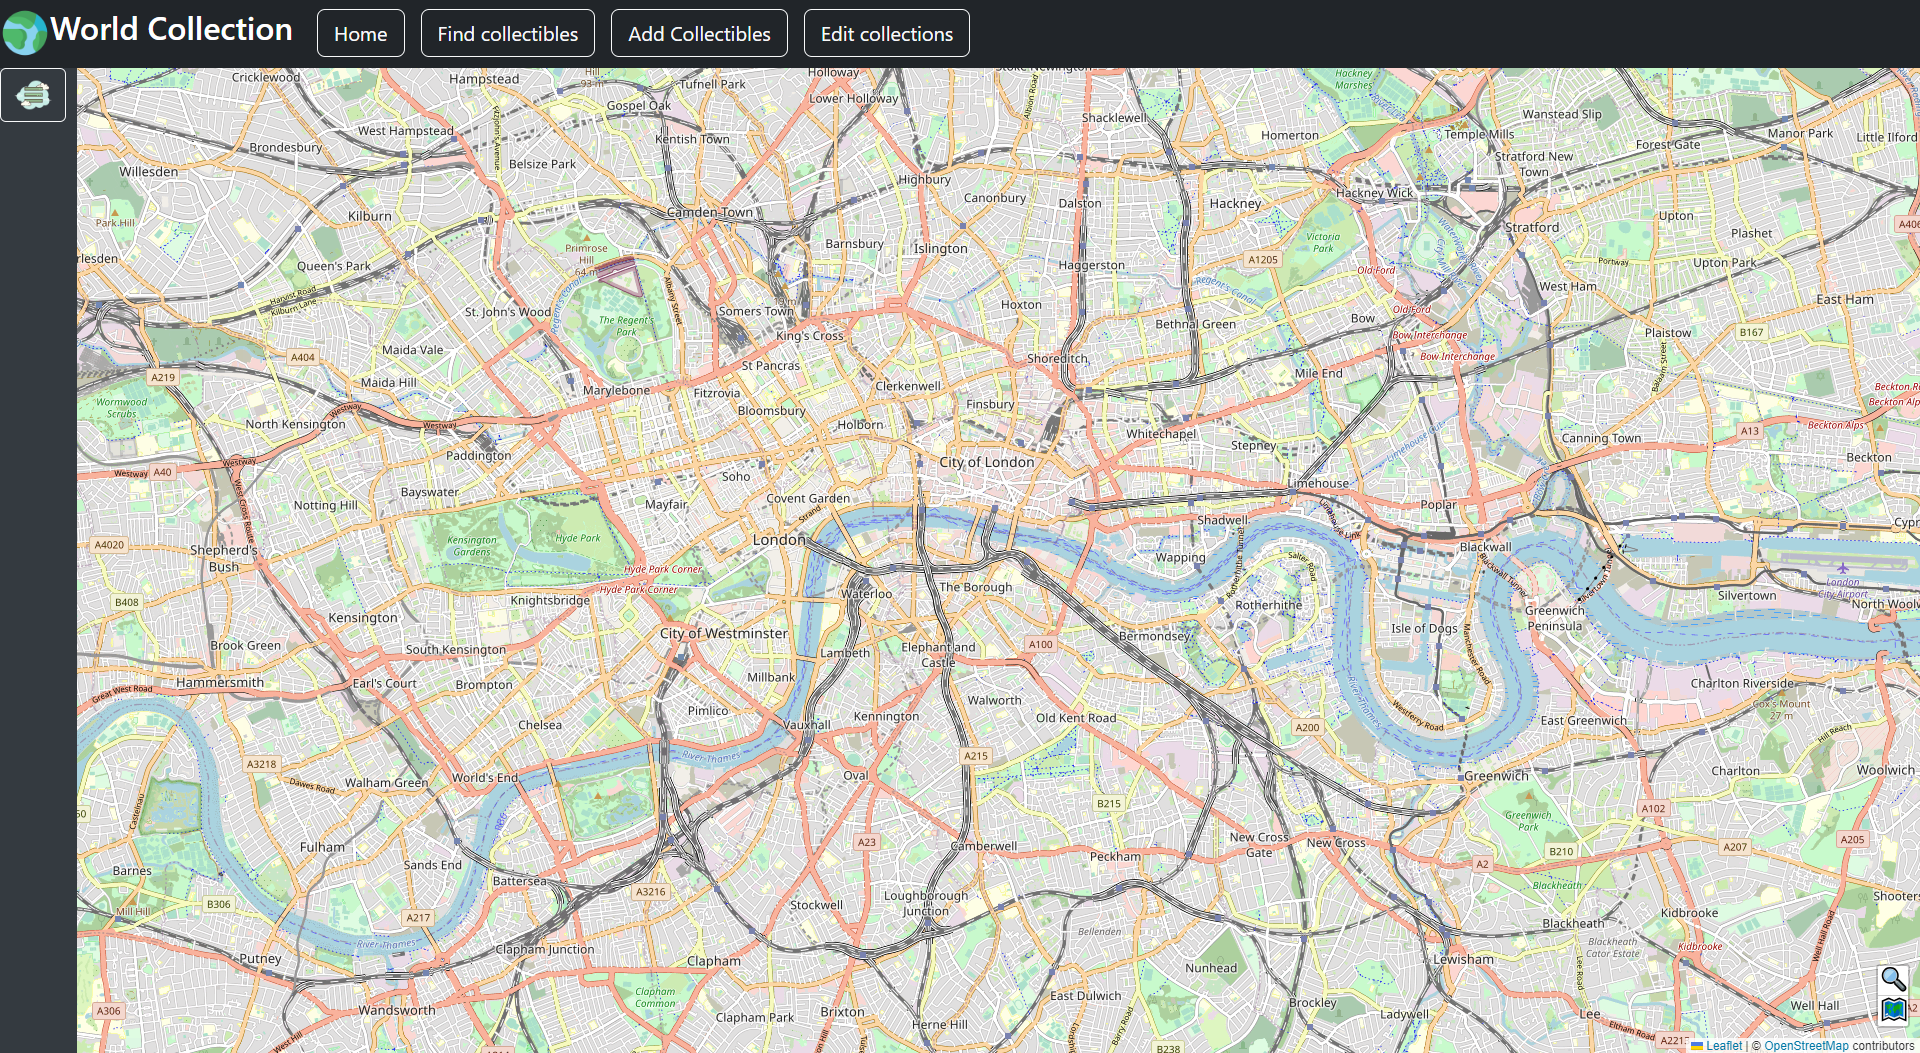
\includegraphics[width=140mm]{../img/ud-prazdna_mapa}
      \centering
      \caption{Vzhľad aplikácia po navštívený stránky}
\end{figure}

Na ľavej strane od mapy nájdeme úzky panel s jedným tlačidlom. Po stlačení tlačidla sa zobrazí namiesto úzkeho panelu širší panel, v ktorom používateľ nájde svoje vytvorené
kolekcie v podobe zoznamu, a šírka mapy sa zmenši. Na zariadeniach s malou obrazovkou je tento panel zobrazený na celu šírku obrazovky a interaktívna mapa nie je zobrazená.
Používateľ je schopný zatvoriť tento panel stlačením červeného tlačidla "X" nachládajúcom sa v pravom hornom rohu panelu. V panely hore nájdeme textové pole, kde môže používateľ
zadať text na základe ktorého sa zobrazujú príslušné kolekcie. Inými slovami používateľ dokáže pomocou tohto vyhľadávať svoje kolekcie.

Každá kolekcia v zozname je reprezentovaná ako informatívny obdĺžnik, kde hore v ľavo je názov kolekcie, a na pravo sa nachádza informácia vyjadrená ako počet navštívených mapových objektov v danej kolekcie ku
počtu všetkých mapových objektov v kolekcii. V dolnej časti je “bar”, ktorý sa vyfarbuje do zelena na základe percenta navštívených objektov. Teda ak používateľ v danej kolekcii nemá navštívený
žiaden mapový objekt tak cely bar je sivý. Ak sú všetky mapové objekty v kolekcii navštívené tak bar je celý naplnený zelenou farbou.

Používateľ môže na obdĺžnik kolekcie kliknúť. Po kliknutí sa na interaktívnej mape zobrazia body reprezentujúce všetky mapové objekty v danej kolekcii.
Pohlaď  mapu sa automaticky nastaví tak aby boli viditeľné všetky body naraz. Po kliknutí na inú kolekciu sa na mape zobrazia body novo kliknutej kolekcii.
Body sú vyfarbené na základe navštívenia daného mapového objektu. Sivé, nevyfarbené body znamenajú, že používateľ ešte nenavštívil daný objekt, kým plne vyfarbené
body reprezentuje, že objekt už bol navštívený.

\begin{figure}[h]
      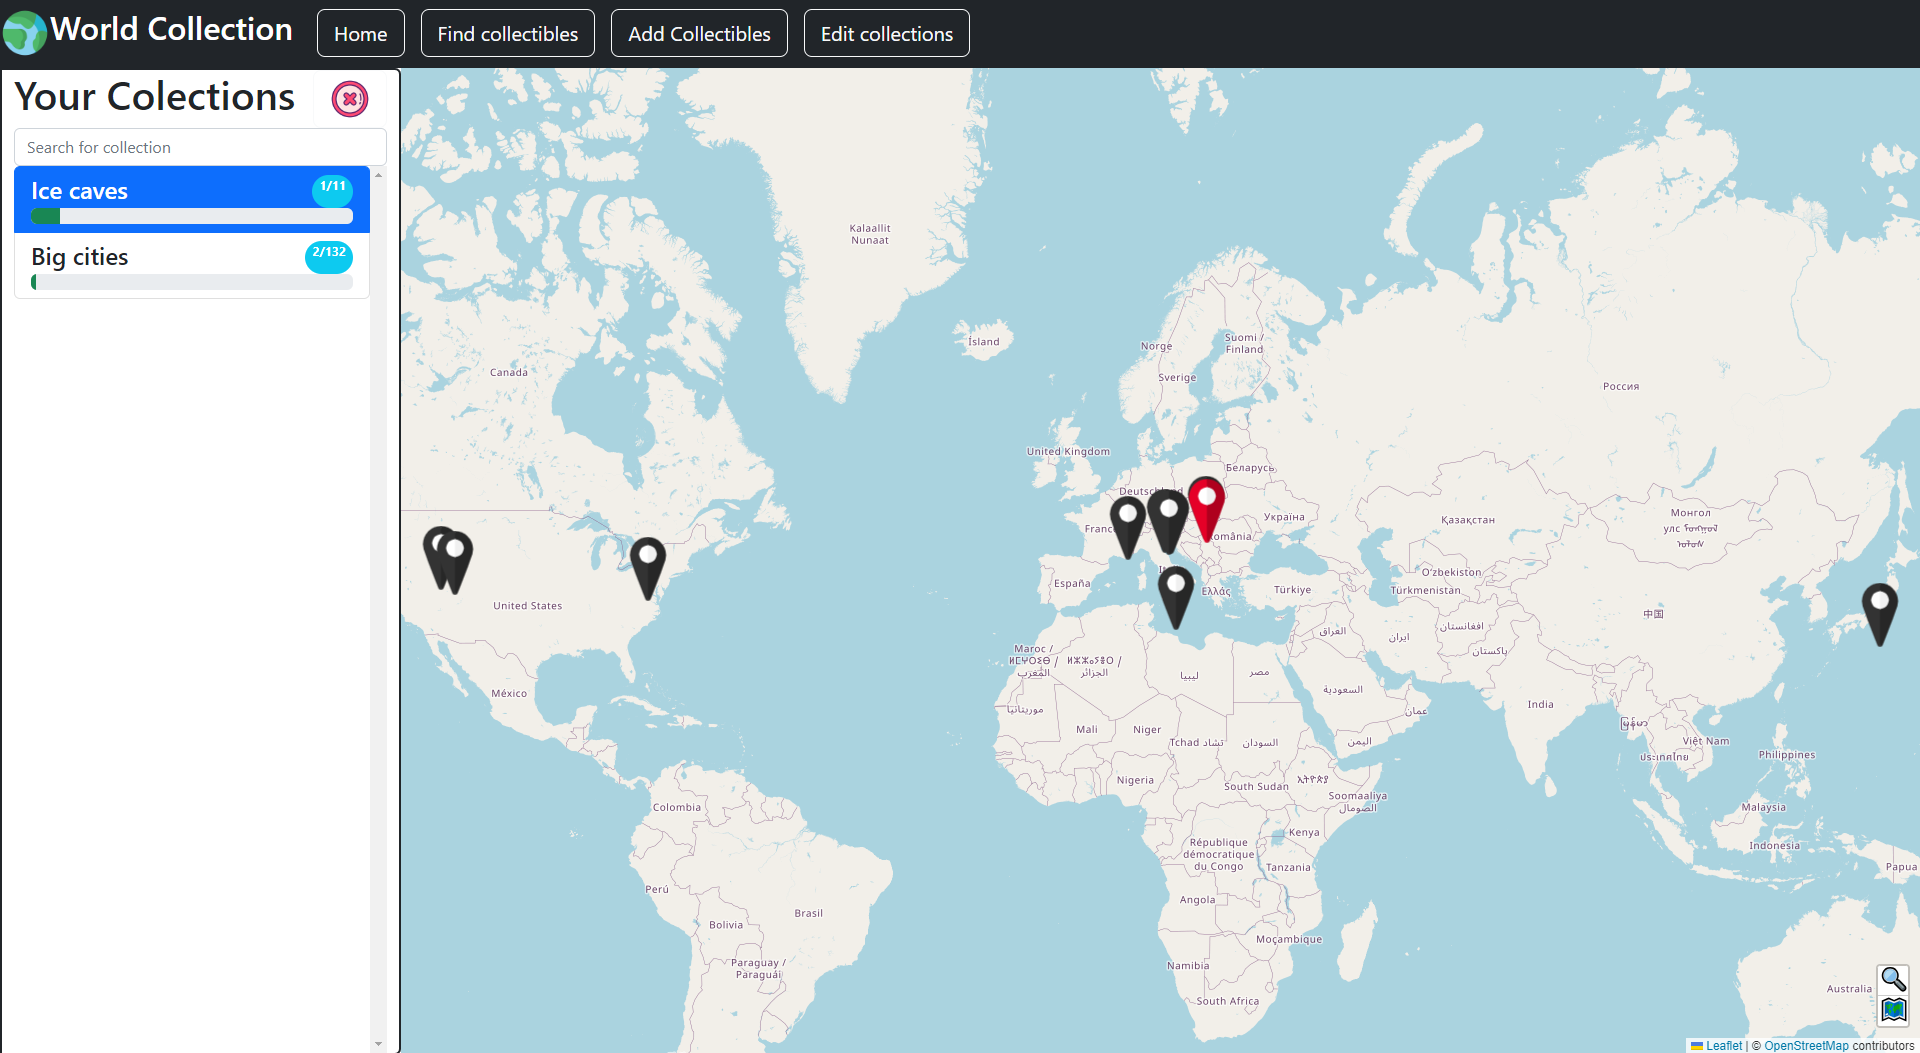
\includegraphics[width=140mm]{../img/ud-mapa-s-bodmy}
      \centering
      \caption{Prezentovanie mapových objektov danej kolekcie}
\end{figure}

Používateľ môže kliknúť na jednotlivý bod na mape. Po tom ako na neho klikne sa na mape tesne nad bodom zobrazí obdĺžnik, v ktorom sú informácie o danom mapovom objekte.
Tento obdĺžnik ma danú veľkosť, z toho dôvodu sa obsah nezmestí cely do obdĺžniku. Používateľ pre prezretie celého obsahu musí v obdĺžniku skrolovať.

\begin{figure}[h]
      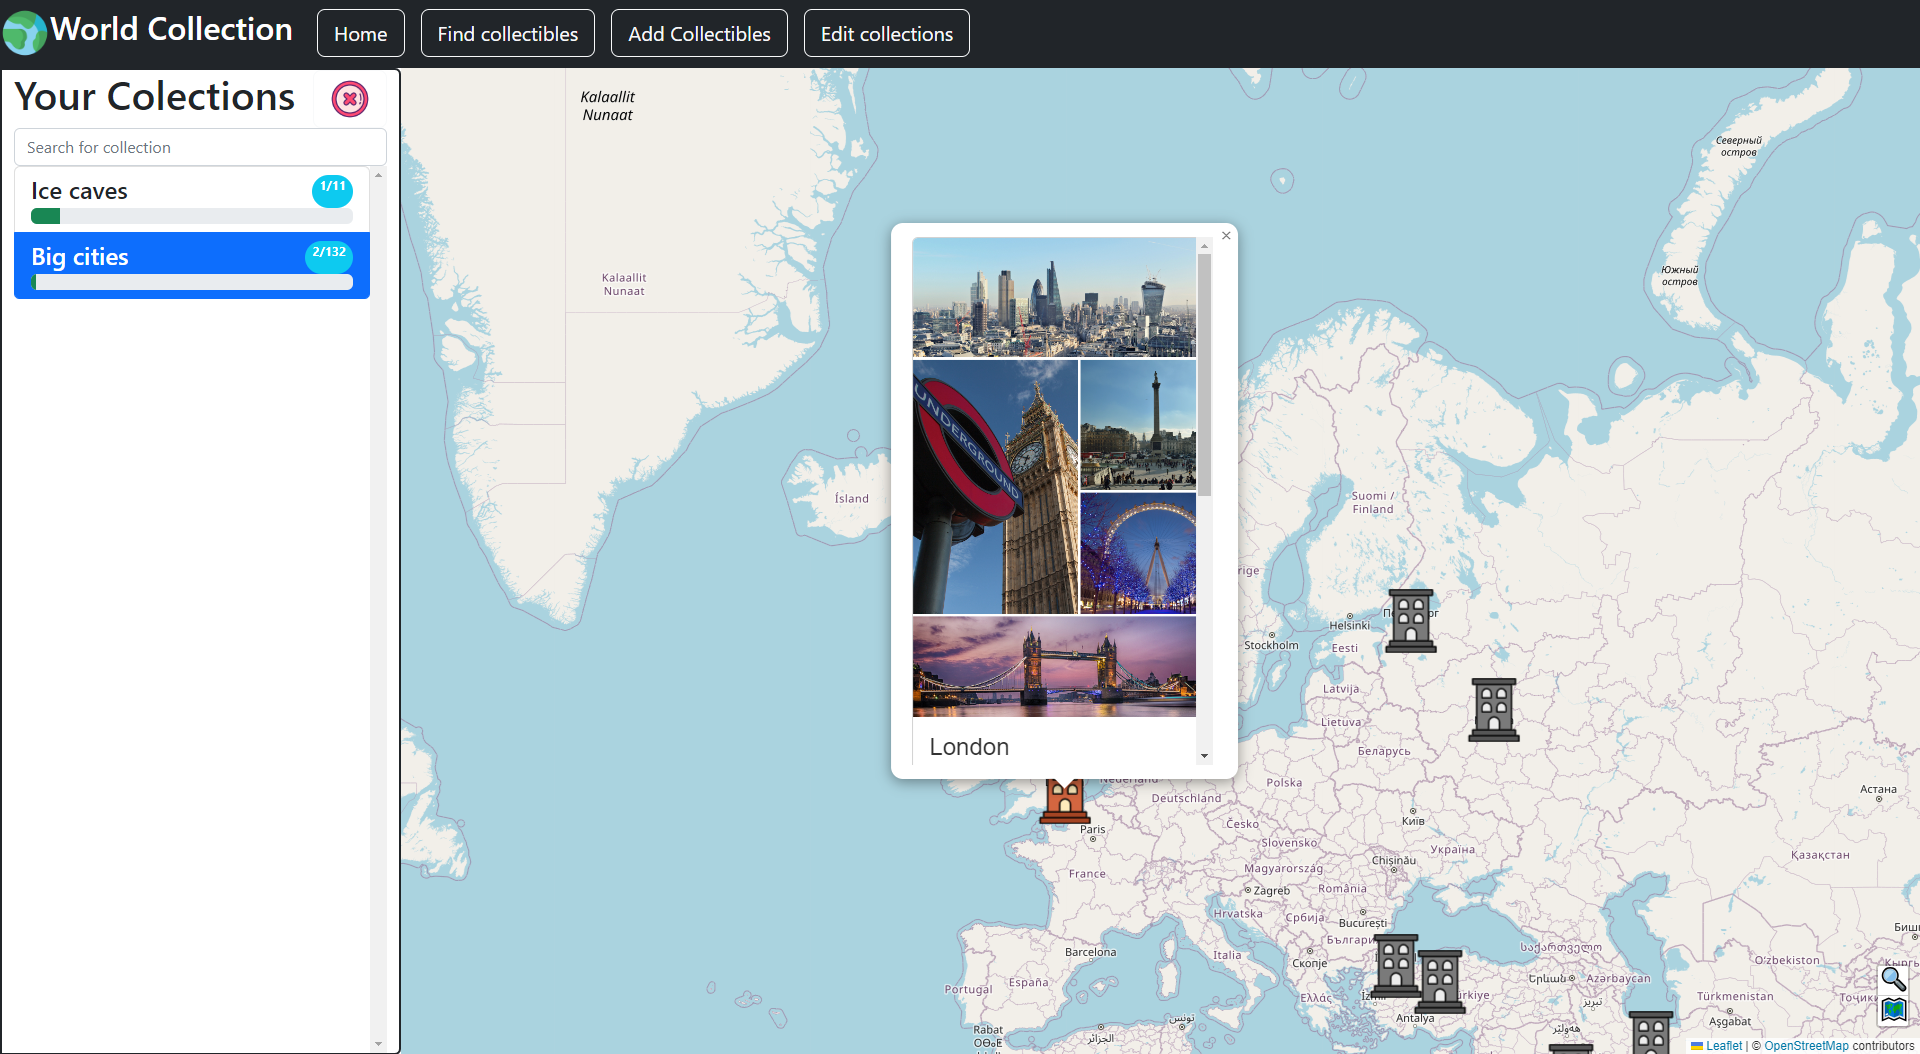
\includegraphics[width=140mm]{../img/ud-obdznik_obrazok}
      \centering
      \caption{Zobrazenie informácii pre daný bod }
\end{figure}

V obdĺžniku na úplnom začiatku je zobrazený obrázok mapového objektu.
Môže nastať situácia, že obrázok nebol nájdený a v takom prípade ho aplikácia nezobrazí. Po obrázku nasledujú informácie ako názov objektu, popis objektu a zoznam jednotlivých "tagov" reprezentujúcich kategórie,
pod ktoré mapový objekt patrí. Napríklad pre mesto "Instanbul" nájdeme tag s informáciou "million city", čo znamená , že objekt je mesto s viac než miliónom obyvateľov.
Ďalej nasleduje status o návšteve objektu. V prípade ak objekt nie je navštívený tak v statuse nájdeme červený obdĺžnik s textom "Not visited yet", v opačnom prípade je to zelený
obdĺžnik s textom "Visited". Pod statusom návštevnosti nájdeme priestor pre poznámky. Ak si používateľ zapíše k objektu poznámky, tak pravé na tomto mieste ich aplikácia zobrazí používateľovi.

Na konci nájdeme akcie mapového objektu. V nich nájdeme štyri pod sebou idúce tlačidla, kde každé z nich po stlačení do obdĺžnika pridá nové časti.
Po stačený daného akčného tlačidla sa text tlačidla zmení na "Close" a po znovu kliknutí na dane tlačidlo, pridaná časť zmizne.

Nasleduje výpis týchto akcii:
\begin{itemize}
      \item "Show details" - zobrazí zoznam s detailmi o mapovom objekte a zároveň odkaz na článok o danom mapovom objekte vedúci na anglickú Wikipédiu, ak článok existuje.
            Detaily sú zobrazené ako zoznam s obdĺžnikmi, kde každý jeden z nich reprezentuje jeden detail. V obdĺžniku je v hornej časti názov detailu a v dolnej časti sú hodnoty daného detailu
            zobrazené ako "tagy". Tagy majú rôznu farbu na základe dátového typu detailu. Zelená je pre hodnoty reprezentujúce čas, oranžova pre kvantitatívne hodnoty a modra pre hodnoty reprezentujúce nejakú
            existujúcu entitu, objekt.
      \item "Visitation" - zobrazí "check box", ktorý používateľ zaškrtne ak daný objekt navštívil. Po zaškrtnutí je zobrazená možnosť zadať dátum návštevy. Ten sa da zadať ako dátum, mesiac s rokom alebo iba ako rok.
            Aplikácia zároveň umožňuje zadať dátum návštevy aj ako časové obdobie definované dvoma dátumami alebo mesiacmi v roku. Spôsob zadania návštevy si používateľ vyberie z výberu možnosti, ktoré mu aplikácia ponúkne a následne zadá návštevnosť.
            Podľa výberu spôsobu zadania návštevnosti sa zobrazia dané vstupné polia pre uvedenie návštevy. Možnosť uviesť aj čas návštevy je voliteľný. Potom ako používateľ zadá potrebné informácie musí pre uloženie kliknúť na zelene tlačidlo s textom "Save".
      \item "edit icon" - zobrazí jednotlivé obrázky, ktoré môžu byť zvolené ako obrázok bodu na mape reprezentujúci daný mapový objekt. Pre nastavenie je postačujúce kliknutie na daný obrázok.
      \item "edit notes" - zobrazí textové pole, do ktorého si môže používateľ zapísať poznámky. V prípade , že k danému objektu sú napísane poznámky, tak sa aktuálny obsah poznámok zobrazí v tomto textovom poli.
            Po napísaní alebo editovaný poznámok musí používateľ pre uloženie poznámok stlačiť zelene tlačidlo s textom "Save notes"
\end{itemize}

\begin{figure}[h]
      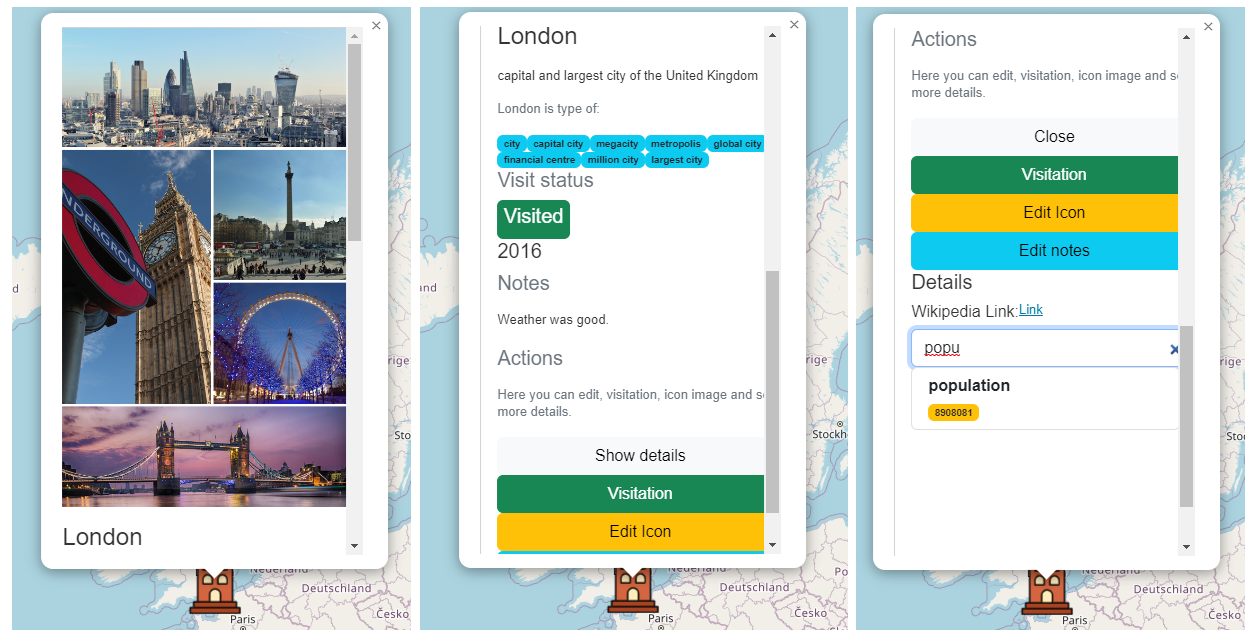
\includegraphics[width=140mm]{../img/ud-obdznik-1}
      \centering
      \caption{Ukážka výzoru časti obdĺžnika zobrazujúcej : obrázok, informácie o objekte, zobrazenie detailov s použitím filtrácie}
\end{figure}

\begin{figure}[h]
      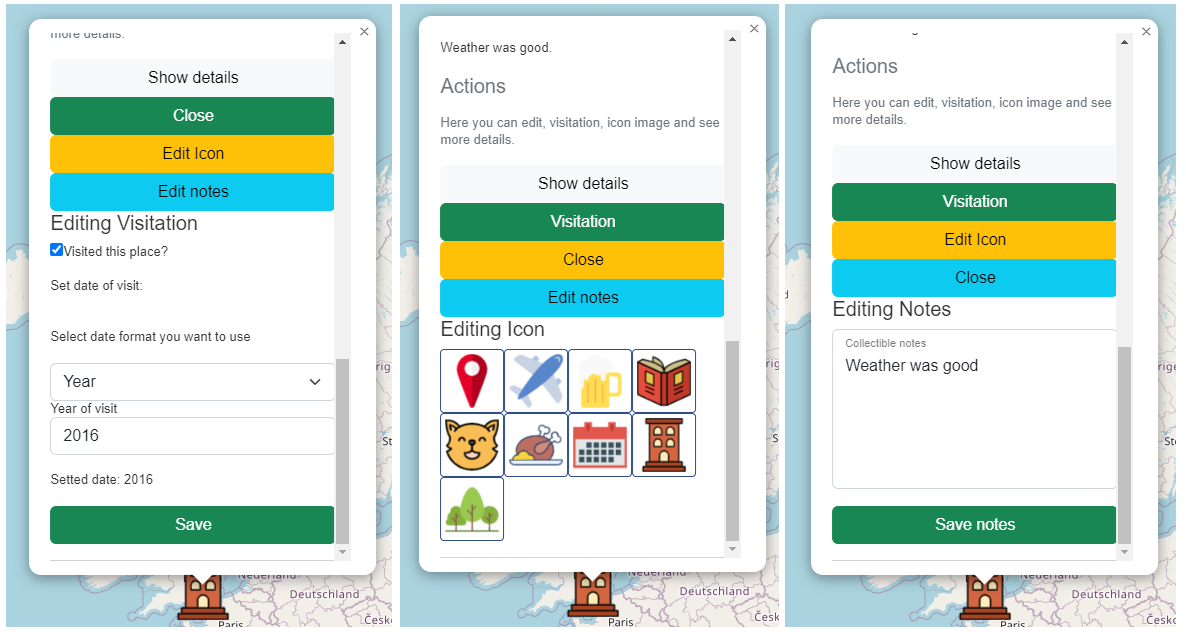
\includegraphics[width=140mm]{../img/ud-obdznik-2}
      \centering
      \caption{Ukážka výzoru časti obdĺžnika zobrazujúcej : nastavovanie návštevnosti, zmena obrázka bodu, editovanie poznámok  }
\end{figure}

\section{Vyhľadávanie mapových objektov }

Tento stav sa zobrazí používateľovi po kliknutí tlačidla s textom "Find collectibles" v hornom navigačnom menu.

V tomto stave používateľ môže zadať jednotlivé parametre, na základe ktorých aplikácia vyhľadá množinu mapových objektov splňujúcich všetky poskytnuté parametre.

Parametre sa zadávajú postupne v jednotlivých krokov. V každom kroku  používateľ je schopnú sa vrátiť o krok naspäť a zadať znovu predchádzajúci parameter.

Jednotlivé kroky sú v nasledujúcich sekciách :

\subsection*{Výber kategórii}
Tento krok zobrazí vyhľadávacie pole, ktoré po zadaní textu začne dynamicky vyhľadávať možné kategórie na základe poskytnutého textu. Nájdene možnosti sú zobrazene v zozname pod týmto vyhľadávacím polom. Vždy je zobrazený názov kategórie a pod nim nasleduje sivou farbou popis danej kategórie.
Kategória je nastavená potom ako používateľ klikne na danú nájdenú možnosť. Je možné nezvoliť žiadnu kategóriu. To používateľ docieli stlačením Žiadne návrhy tlačidla "Anything". Po tom ako je kategória vybraná môže používateľ pokračovať na ďalší krok stlačením zeleného tlačidla s textom "Continue“ alebo
vybrať inú kategóriu stlačením modrého tlačidla "Choose other". Ešte pred tým ako používateľ klikne na tlačidlo "Continue", si môže vybrať jednu alebo viac pod-kategórii, ktoré reprezentujú to, že nájdene objekty nesmú byť tejto kategórie.
Vyhľadávanie funguje rovnako ako pri kategórii až na to, že v tomto prípade vo vyhľadávacom poli na začiatku je aj tlačidlo "Show all". Po stlačený tohto tlačidla aplikácia vyhľadá úplne všetky možné pod-kategórie zvonnej kategórii.
\begin{figure}[h]
      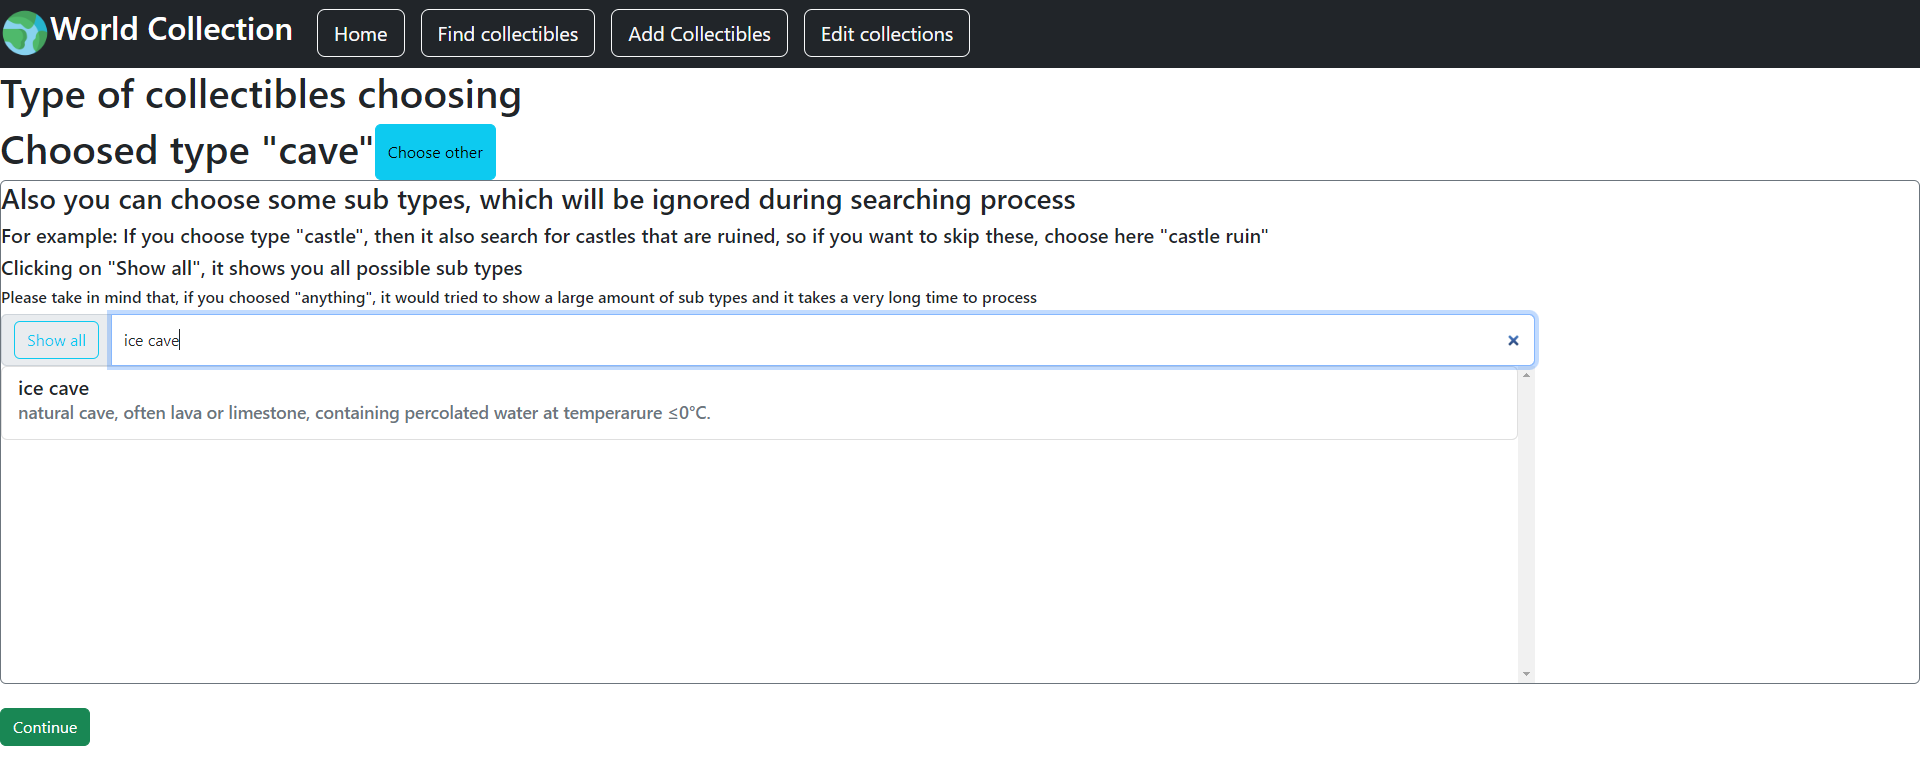
\includegraphics[width=140mm]{../img/ud-kategoria.png}
      \centering
      \caption{Ukážka výberu kategórie. Používateľ vybral kategóriu "cave" a následne vyhľadáva pod-kategórie s názvom "ice cave". }
\end{figure}

\subsection*{Vyber spôsobu zadania oblasti a definovanie oblasti}
Tento krok zobrazí najprv štyri možnosti na výber spôsobu definovania oblasti, v ktoré sa musia nachádzať hľadané objekty. Po tom ako používateľ klikne na danú možnosť pomocou tlačidla “Use” aplikácia zobrazí potrebné prostriedky pre zadanie oblasti.
\begin{figure}[h]
      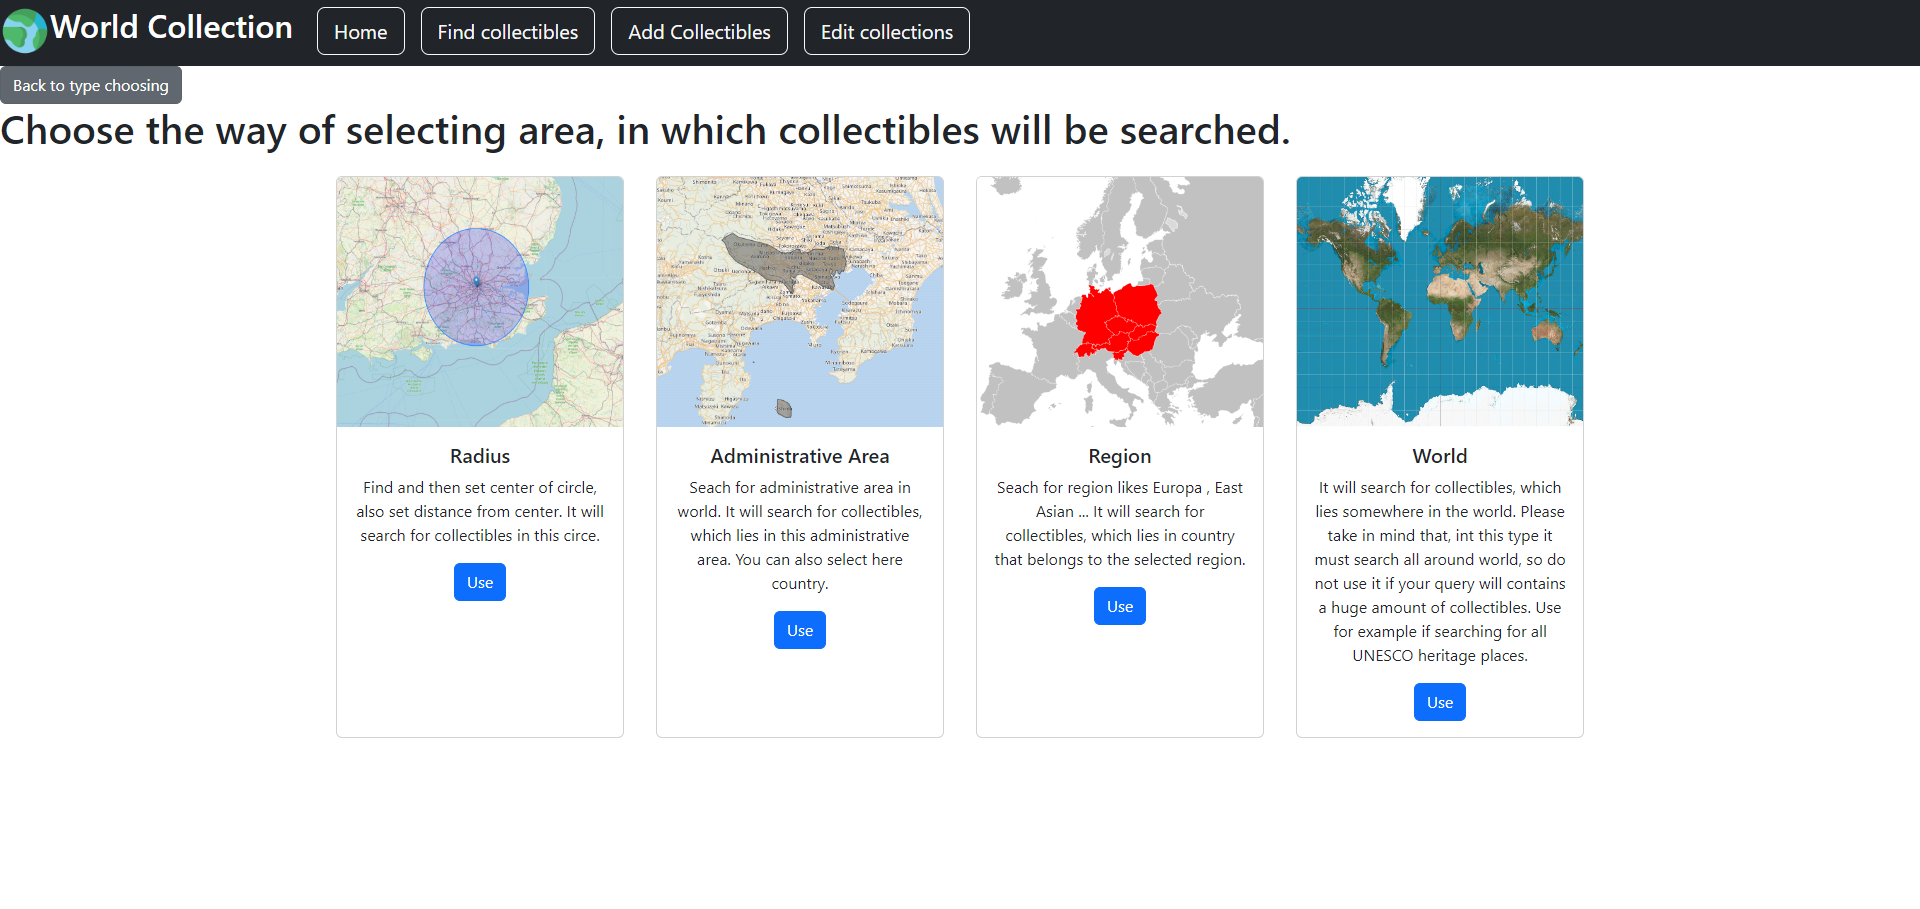
\includegraphics[width=140mm]{../img/ud-vyber-oblasti.png}
      \centering
      \caption{Vyber spôsobu zadania oblasti.}
\end{figure}
Nasledujú výpis týchto možnosti:
\begin{itemize}
      \item Radius - zobrazí interaktívnu mapu s jedným bodom na mape a modrým okruhom okolo bodu. Modry kruh reprezentuje oblasť, v ktorej sa bude vyhľadávať.
            Bod je možne presúvať chytením a posúvaním po mape. Na ľavo od mapy je zobrazený panel, v ktorom sú tri tlačidla. Jedno vráti používateľa na vyber spôsobu zadania oblasti,
            druhé pokračuje na ďalší krok a tretí zobrazí širší panel, v ktorom môže používateľ nastaviť polomer kruhu. Ten sa nastaví posúvaním bodu v bare. Rozsah je od 1km po 250 km.
            Tento širší panel zároveň ponúka možnosť na základe názvu vyhľadať lokáciu mapového objektu, na ktorý sa bod určujúci stred kruhu presunie.
            \begin{figure}[h]
                  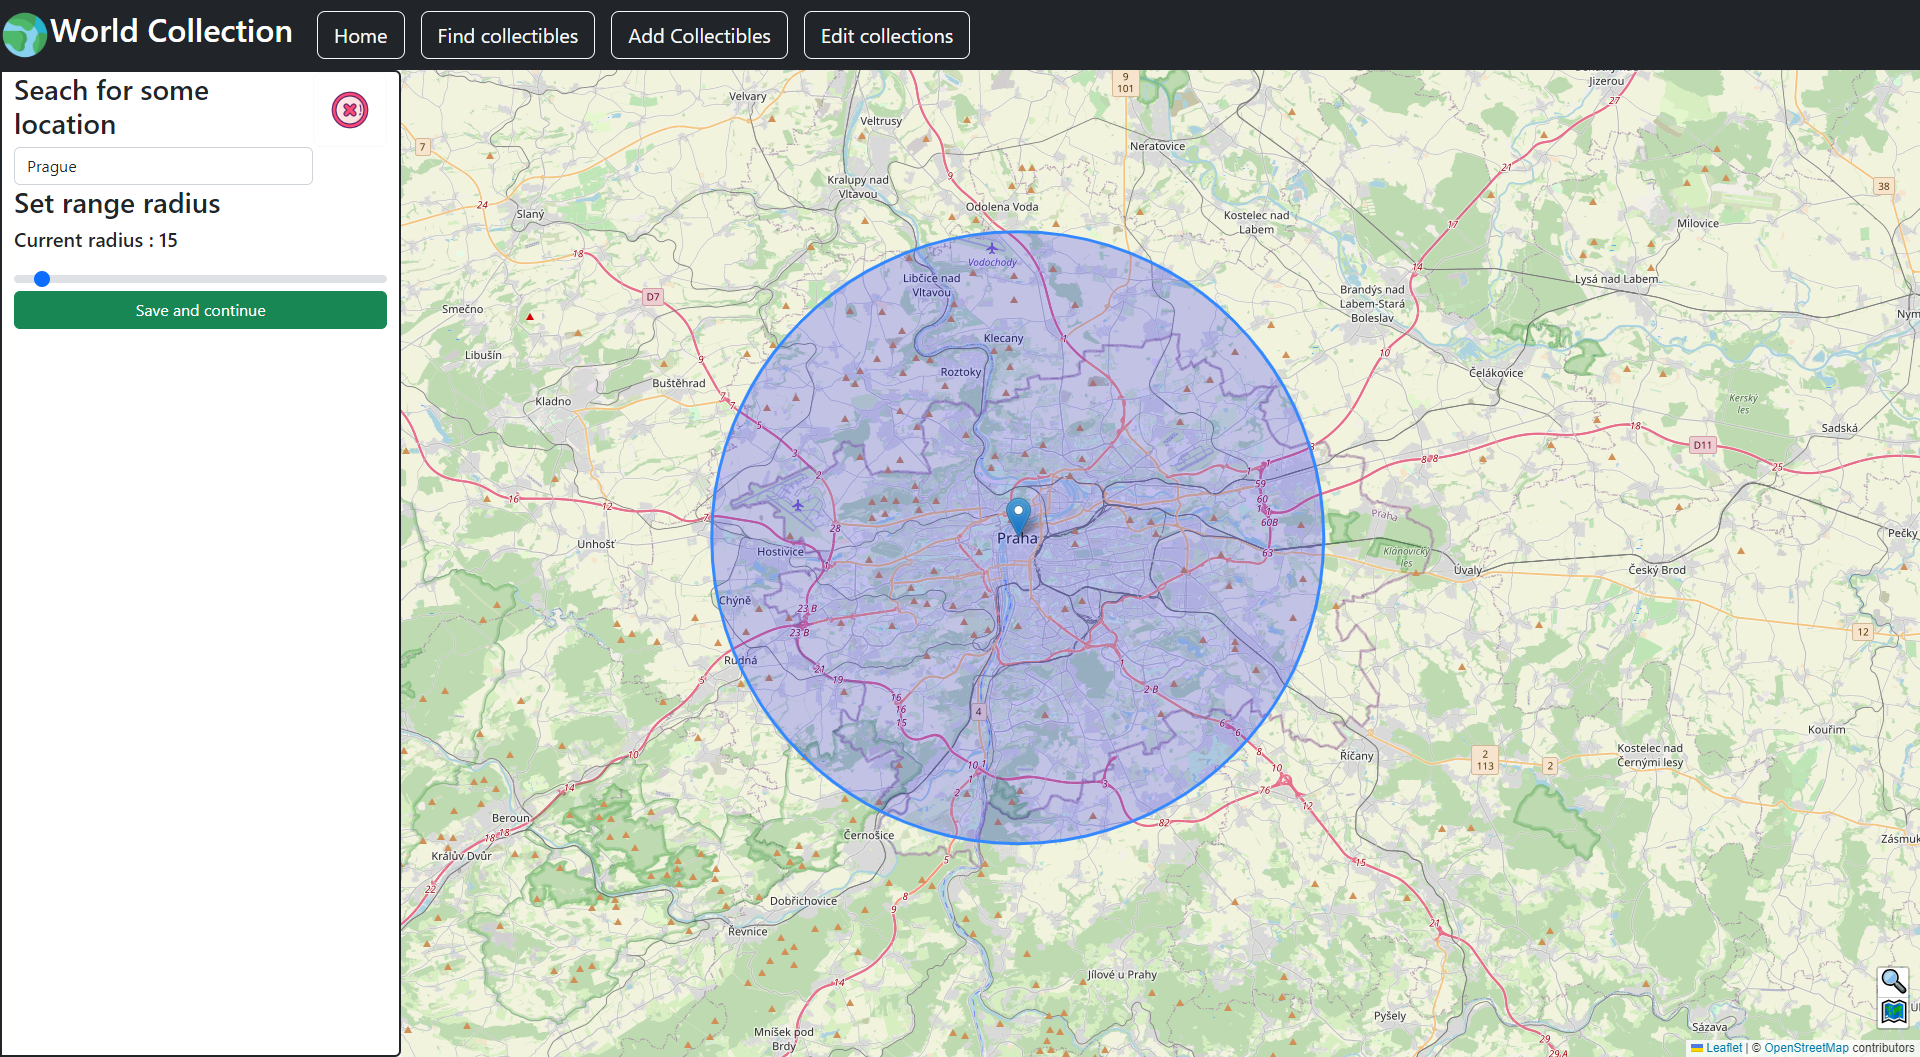
\includegraphics[width=140mm]{../img/ud-radius.png}
                  \centering
                  \caption{Ukážka zadania oblasti vyhľadávania okolo bodu.}
            \end{figure}
      \item Administratívne územie - zobrazí vyhľadávacie pole, ktoré vyhľadáva súčasne administratíve územia, pod ktoré spadajú aj jednotlivé štáty. Vyhľadanie a spôsob výberu je rovnaký ako u vyhľadávaní kategórii.
            Potom ako je územie vybrane aplikácia umožni používateľovi zadať aj administratívne územia, ktoré spadajú pod vybraté administrovane územie, ako výnimky. To znamená, že hľadané mapové objekty
            sa musia nachádzať vo zvolenom administratívnom území, ale zároveň nepatria do administratívneho územia definovaného ako výnimka.
      \item Región - zobrazí vyhľadávacie pole, ktoré vyhľadáva veľké územne celky ako regióny. Napríklad "Európa", alebo "stredná Európa". Vyhľadávacie pole obsahuje aj tlačidlo "Show all", po stlačení ktorého sa vyhľadajú všetky možne možnosti zadania regiónu.
      \item cely svet - nezobrazí nič, pretože cely svet nie je potrebne definovať a rovno sa preskočí na ďalší krok
\end{itemize}

\subsection*{Aplikácia filtrov}
V tomto kroku používateľ môže aplikovať jednotlivé filtre na vyhľadávanie.
Kazdy filter reprezentuje nejakú vlažnosť ako napríklad "nadmorská výška", "populácia" a podobne. Nájdene mapové objekty musia zadanú vlastnosť spĺňať.
Aplikácia v tomto kroku zobrazí na ľavej strane úzky panel s možnosťami na pokračovanie na ďalší krok, vrátenie sa na vyber oblasti,
zobrazenie zoznamu možných filtrov a zoznam už aplikovaných filtrov.
V zozname filtrov si môže používateľ vybrať, či chce aby boli zobrazene odporúčane filter pre danú zadanú kategóriu, alebo všetky možne filtre. Prepínanie medzi odporúčanými a všetkými filtrami je uskutočnené pomocou tlačidla "Filters".
Filtre sa dajú vyhľadávať pomocou vyhľadávacieho poľa. Každý filter obsahuje svoj názov , popis a na ľavej strane aj tag reprezentujúci typ filtra.
Po kliknutí na filter sa zobrazia prostriedky na zadanie hodnoty daného filtru. Pre každý typ filtra sa zobrazia iné prostriedky.
\begin{figure}[h]
      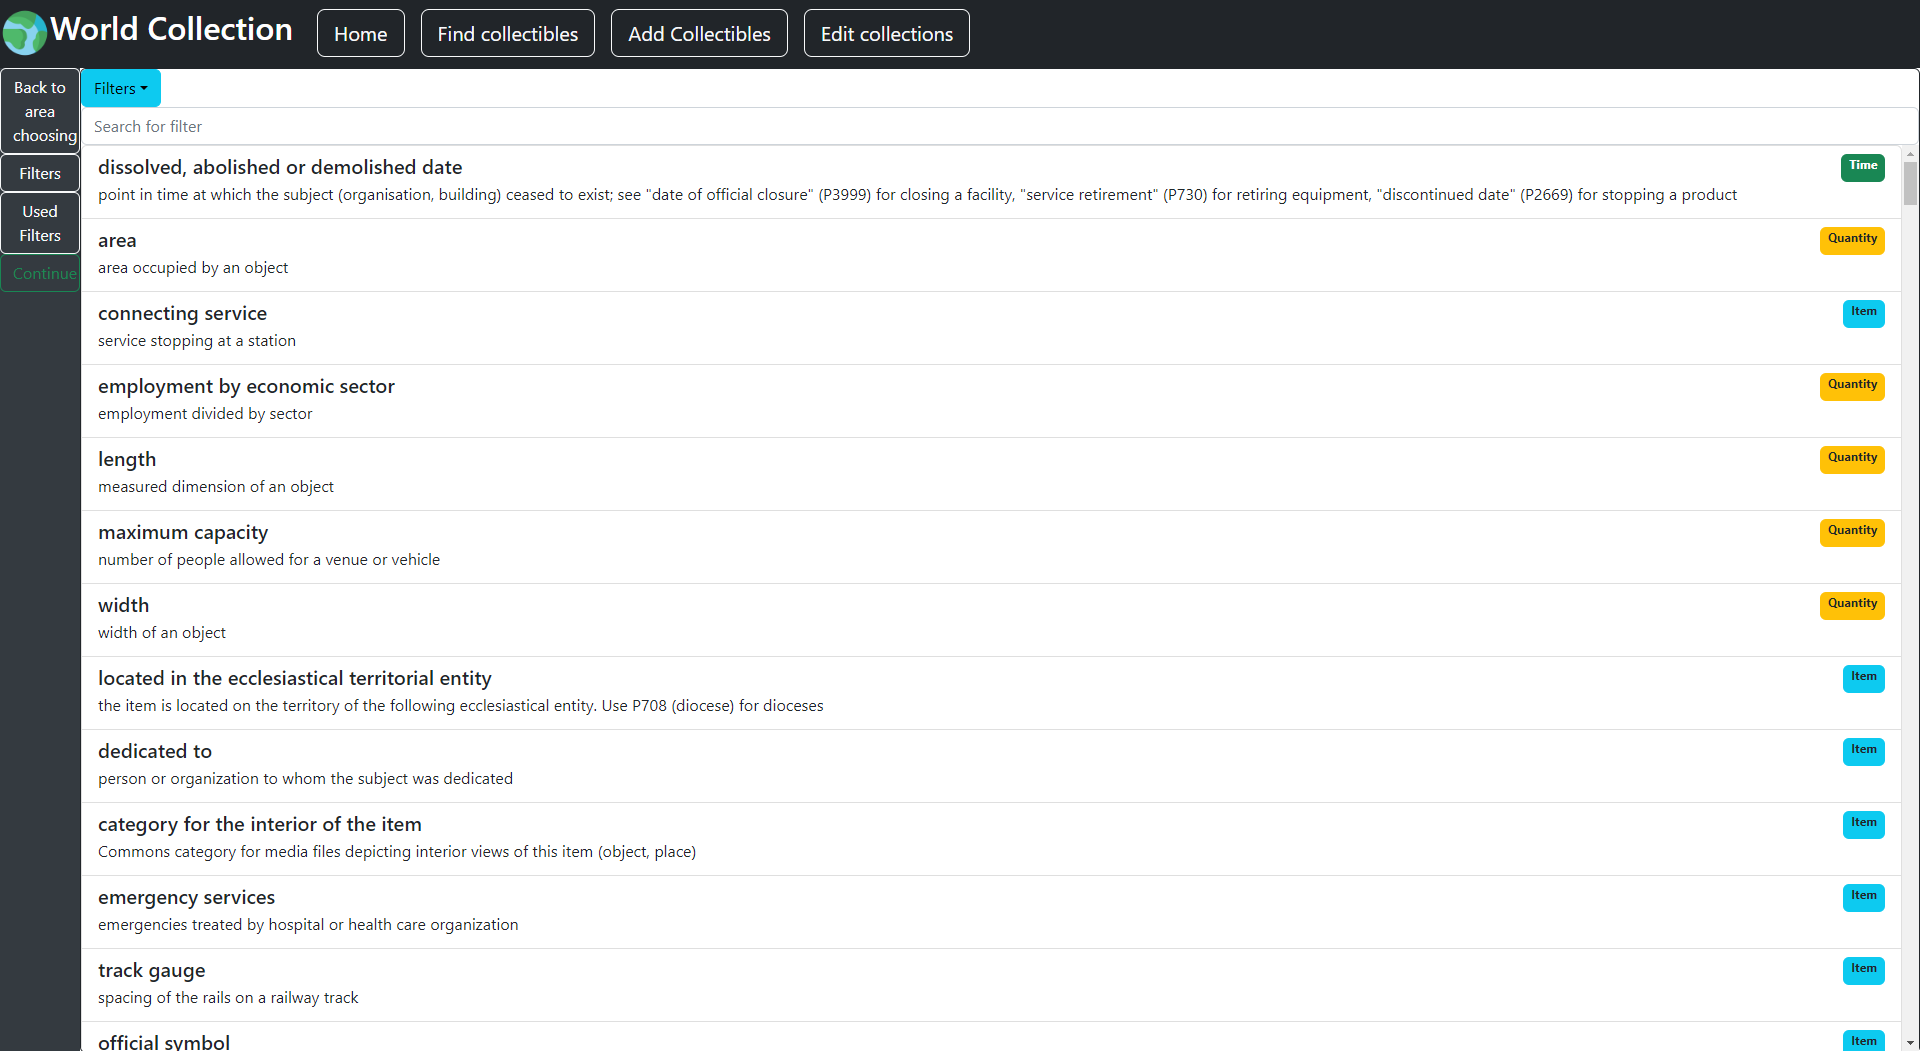
\includegraphics[width=140mm]{../img/ud-vyber-filtrov.png}
      \centering
      \caption{Zoznam “všetkých filtrov”.}
\end{figure}
Výpis typov filtra:
\begin{itemize}
      \item "item" - zadávanie hodnoty ako entita, objekt. Zobrazí buď selektor s možnosťami, ktoré sa dajú použiť ako hodnota filtru, alebo vyhľadávacie pole, v ktorom vie používateľ vyhľadať jednotlivé entity, objekty vhodné na požutie pre daný filter.
            \begin{figure}[h]
                  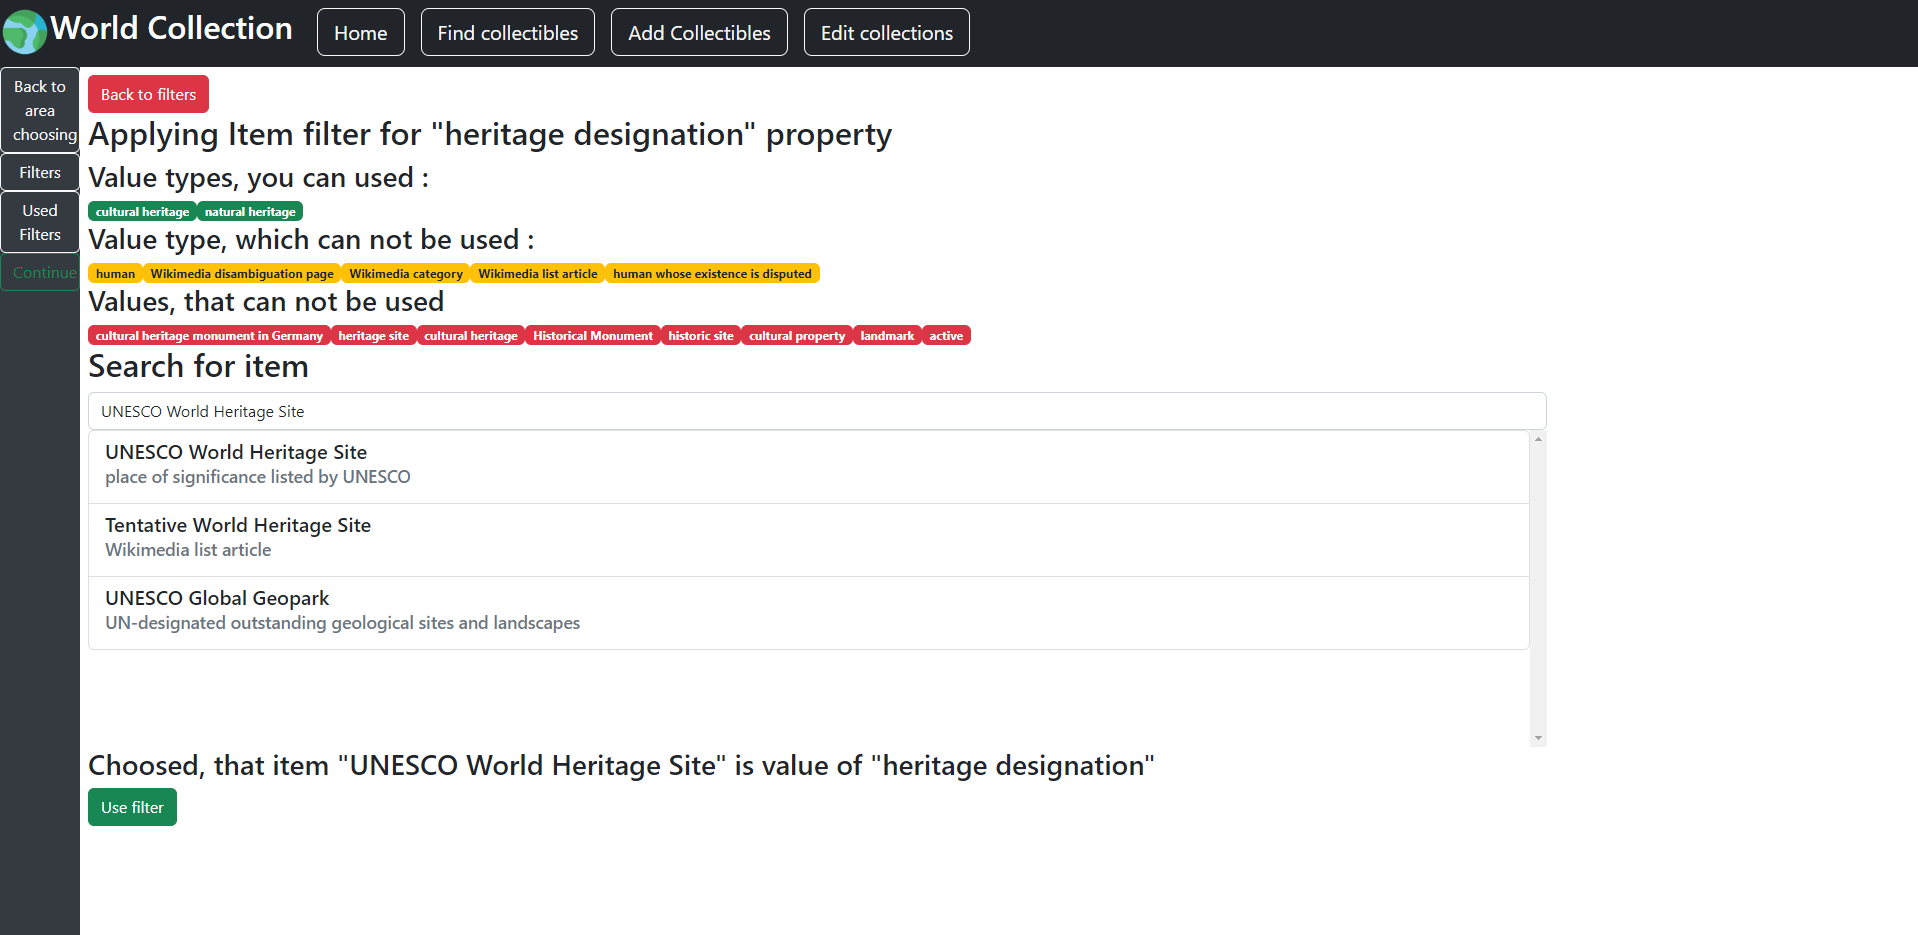
\includegraphics[width=140mm]{../img/ud-item-filter.png}
                  \centering
                  \caption{Ukážka zadania filtru.  Filter "kultúrne dedičstvo" s hodnotou "UNESCO" nájde objekty patriace do zoznamu UNESCO}
            \end{figure}
      \item "quantity" - zadávanie hodnoty ako desatinne číslo pomocou vstupného poľa, v danom rozsahu, ktorý je zobrazení taktiež používateľovi.
            Aplikácia zároveň zobrazí selektor s možnosťami porovnávacích operátov. Zvolený z nich bude použitý vo filtri.
            Pre niektoré filtre zobrazí aplikácia pomocou selektoru aj možnosť zadať jednotku , v ktorej bude zadaná hodnota vyjadrená.
            \begin{figure}[h]
                  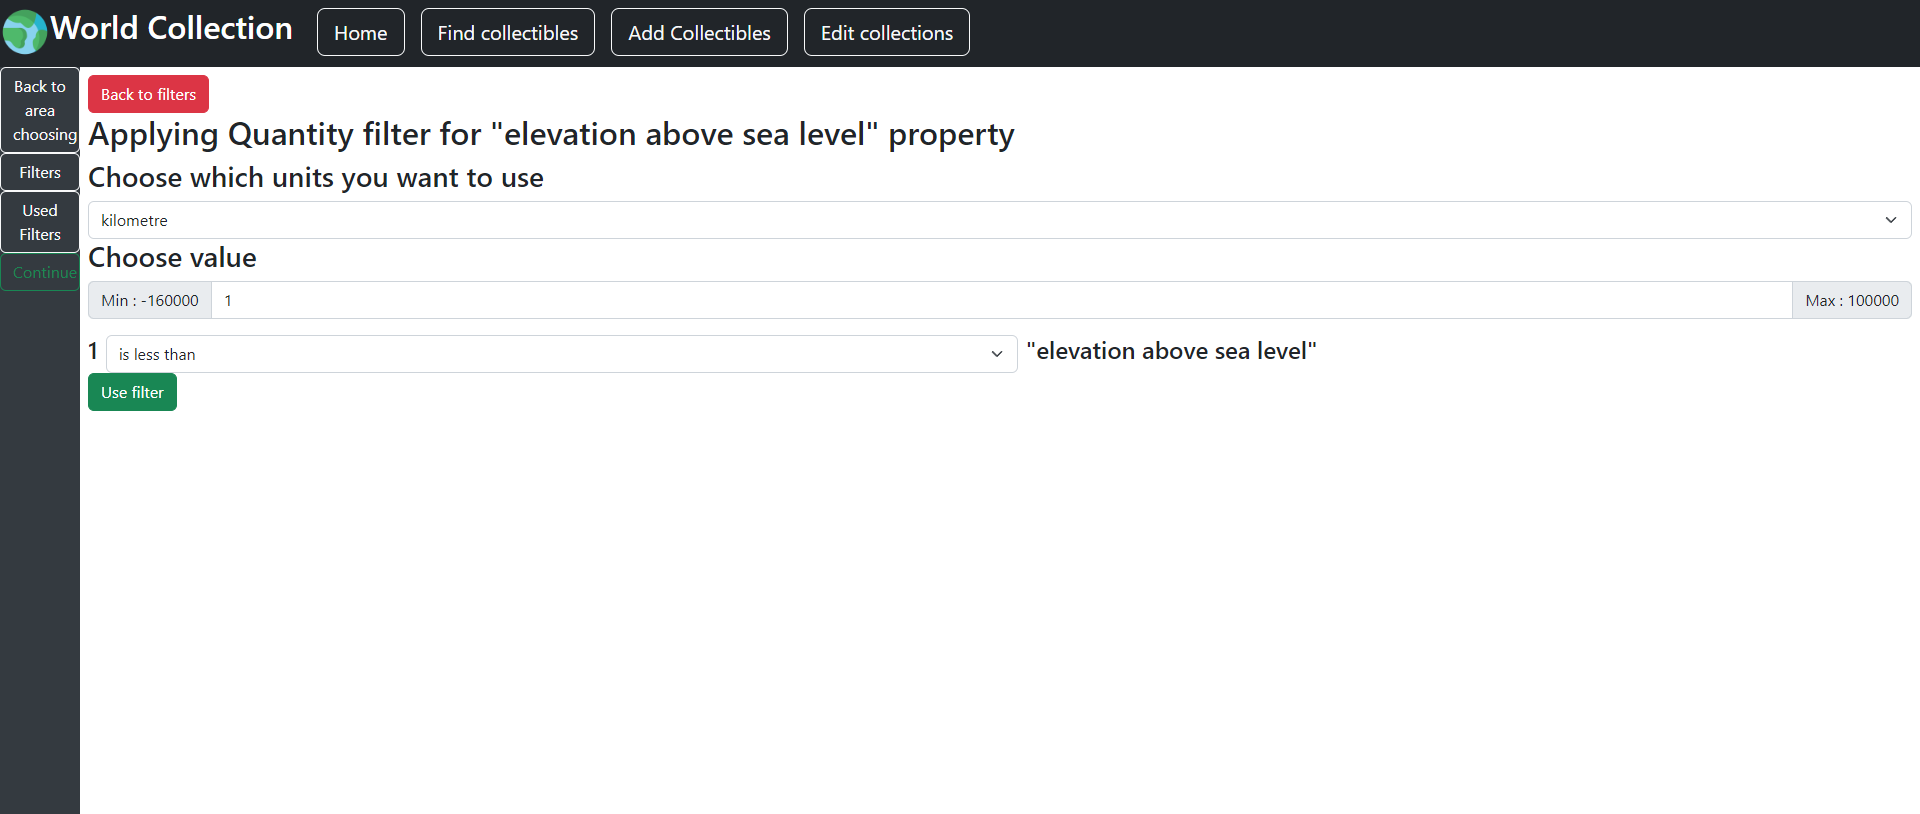
\includegraphics[width=140mm]{../img/ud-quantity-filter.png}
                  \centering
                  \caption{Ukážka zadania filtru. Filter "nadmorská výška" , zadaná hodnota "1" , zvolené jednotky "kilometre" a operátor "menši než" nájde objekty, ktorých nadmorská výška je
                        väčšia ako 1000 metrov.}
            \end{figure}
      \item "Time" - zadanie hodnoty ako bodu v čase. Aplikácia zobrazí selektor s možnosťami zadania času. Čas sa dá vyjadriť ako dátum, mesiac a rok, rok alebo ako storočie.
            Na základe vybratej možnosti aplikácia zobrazí vhodne vstupné polia na zadanie času.
            Aby bol filter možne aplikovať je potrebne aby používateľ vybral zo selektoru porovnávací operátor, ktorý sa použije vo filtri.
            \begin{figure}[h]
                  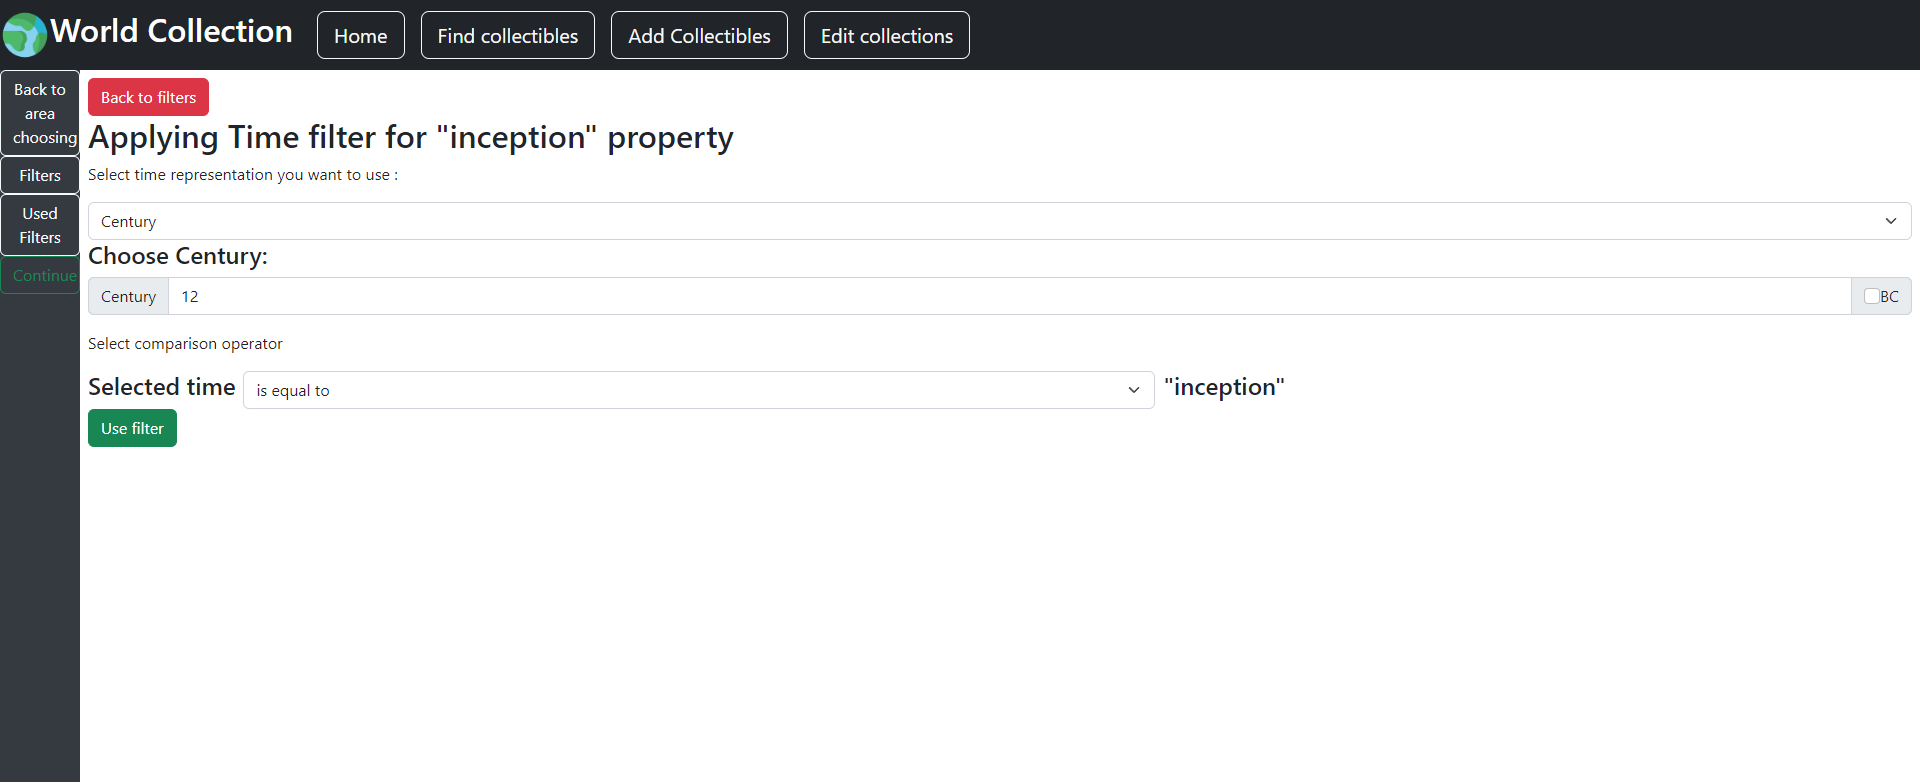
\includegraphics[width=140mm]{../img/ud-time-filter.png}
                  \centering
                  \caption{Ukážka zadania filtru. Filter "vznik" s hodnotou "12. storočie" a porovnávacím operátom "rovná sa" nájde objekty ktoré vznikli v 12. storočí.}
            \end{figure}
\end{itemize}
V zozname použitých filtrov si môže používateľ pozrieť aké filtre sú už aplikované, alebo ich zrušiť pomocou tlačidla s textom ”remove”.

\subsection*{Prehlaď výsledkov}
Po poslednom kroku začne aplikácia vyhľadávať na základe poskytnutých parametrov mapové objekty.
Ak vyhľadávanie neskonči do 60. Sekúnd, aplikácia preruší vyhľadávanie a informuje o tom používateľa.
V opačnom prípade vyhľadávanie skonči a nájdene mapové objekty sa zobrazia používateľovi buď v tabuľke, alebo ako body na interaktívnej mape.
Spôsob prezentácie nádejných mapových objektov si vie používateľ vybrať pomocou tlačidla "View".
Nájdené mapové objekty si vie používateľ filtrovať na základe mena alebo kategórie pomocou textových poli poskytnutých aplikáciou.
Každý nájdený mapový objekt môže používateľ tlačidlom "Remove" zmazať s množiny nájdených mapových objektov, editovať jeho meno stlačením tlačidla "Edit", alebo zobraziť detaily mapového objektu tlačidlom "Show details".
V mapovom pohľade sa informácie a detaily zobrazia po kliknutí na bod reprezentujúci daný mapový objekt.
Aplikacia ponuka moznost vratit cinnost editovanania , alebo zmazania pomocou tlacidla "Undo".

\begin{figure}[h]
      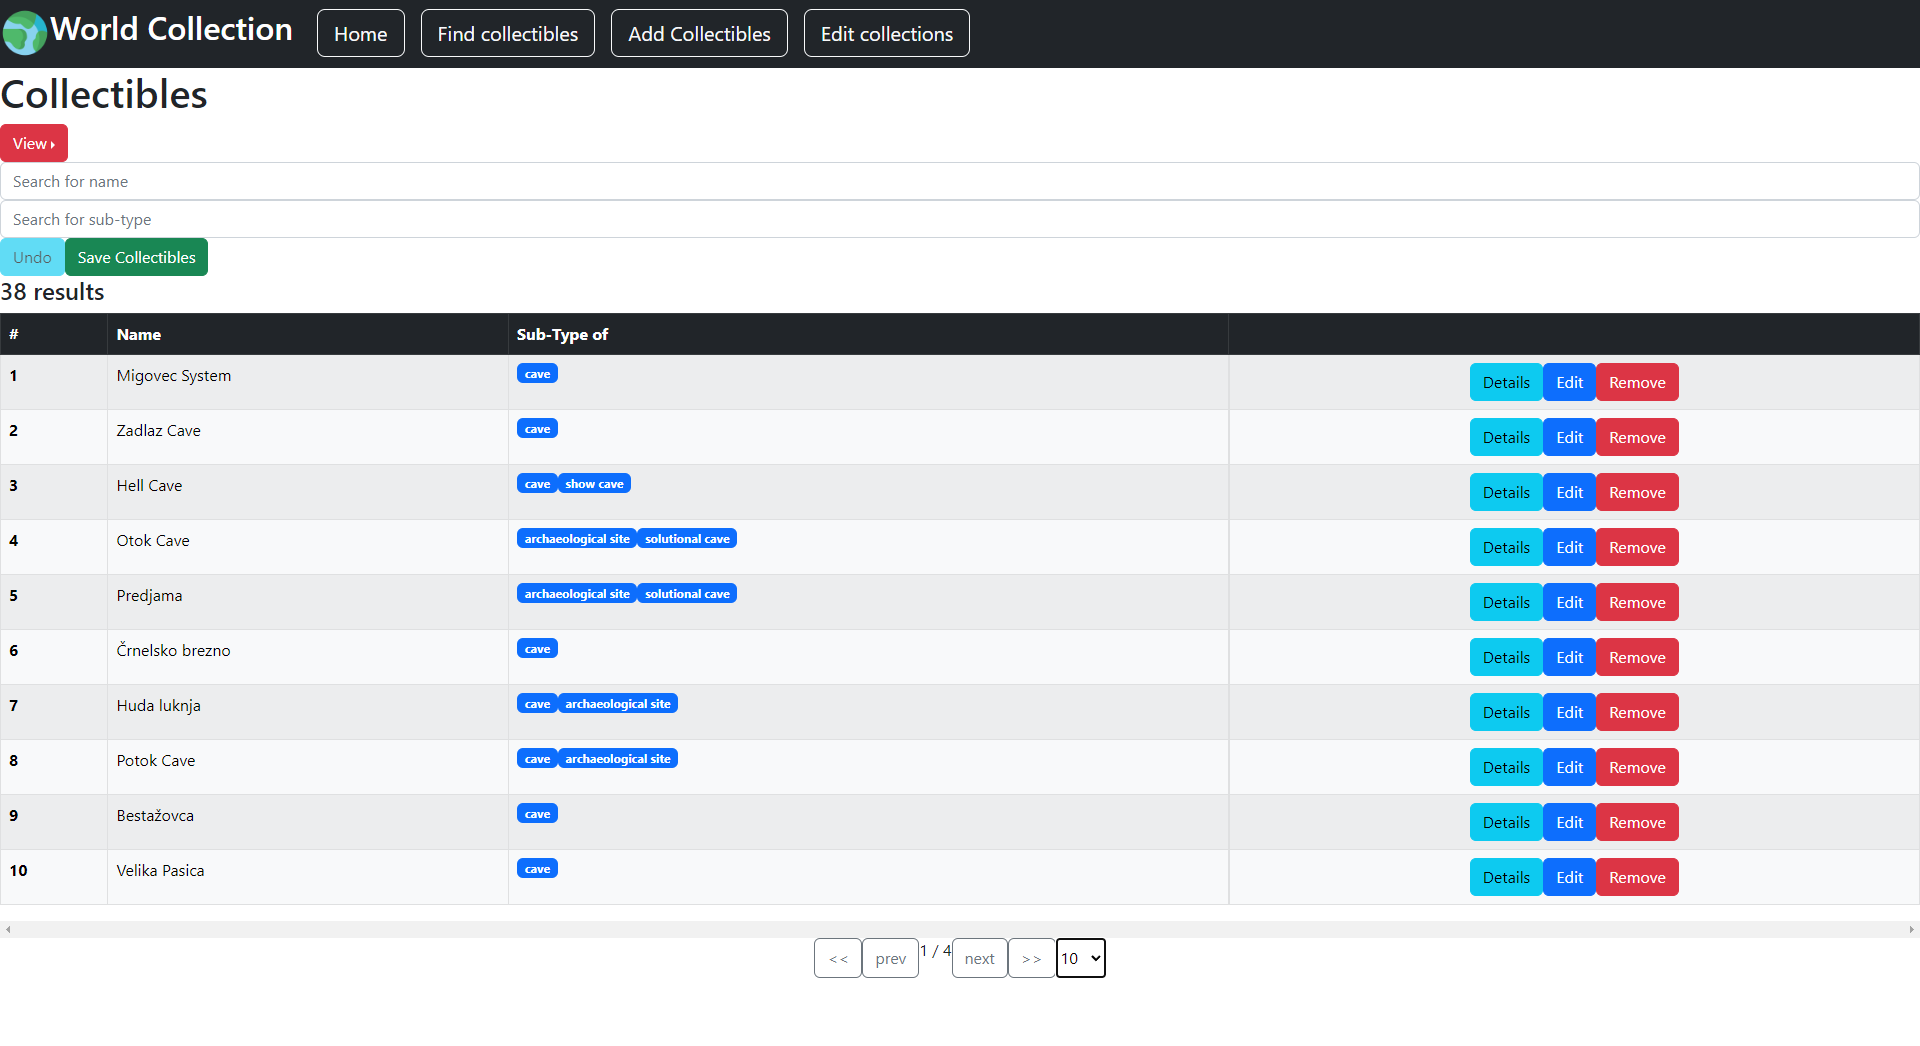
\includegraphics[width=140mm]{../img/ud-vysledok.png}
      \centering
      \caption{Ukážka výsledkov vyhľadania v tabuľke.}
\end{figure}

Po tom ako používateľ je spokojný z množinou, si objekty v nej následne môže uložiť pomocou tlačidla "Save Collectibles".
Toto tlačidlo zobrazí selektor s výberom existujúcich kolekcii, do ktorých môžu byť mapové objekty uložené.
v prípade, že používateľ chce vytvoriť novu kolekciu a do nej uložiť objekty, tak stlačí tlačidlo "Create new Collection".
Aplikácia zobrazí vstupne textové pole, kde používateľ zadá názov novej kolekcie a následne ju uloží tlačidlom "Save". Potom sa vráti
naspäť do výberu kolekcii, kde už bude na vyber aj novo vytvorená kolekcia.

\section{Pridávanie mapových objektov }

Tento stav sa zobrazí používateľovi po kliknutí tlačidla "Add collectibles" v hornom navigačnom menu.

V tomto stave si používateľ na základe názvu vyhľadá mapový objekt, ktorý si následne môže uložiť do niektorej zo svojich kolekcii.

Aplikácia zobrazí interaktívnu mapu sveta a na ľavej strane od nej zobrazí úzky panel s jedným tlačidlom. Po stlačení tohto tlačidla sa panel rozšíri. V rozšírenom panely je vyhľadávacie textové pole na vyhľadávanie mapových objektov.
Po tom ako používateľ vyhľadá a zvoli mapový objekt sa na mape zobrazí bod reprezentujúci daný mapový objekt. Zároveň sa pohlaď mapy zmení tak aby pohlaď bol sústredený na tento bod. Zvolený bod sa dá následne tlačidlom
"Add", v tom istom panely, pridať do zoznamu mapových objektov. Ten je zobrazený v panely pod vyhľadávacím textovým polom. Pridaný mapový objekt v zoznamu dokáže používateľ tlačidlom "Remove" odobrať. Na spodku panelu je zelene tlačidlo "Save Collectibles",
ktoré sa ale zobrazí iba ak je aspoň jeden mapový objekt pridaný do zoznamu. Po kliknutí na tlačidlo sa používateľovi zobrazí rovnako ako u ukladania nájdených mapových objektov
možnosť na uloženie objektov do kolekcii alebo vytvorenie novej kolekcii.

\begin{figure}[h]
      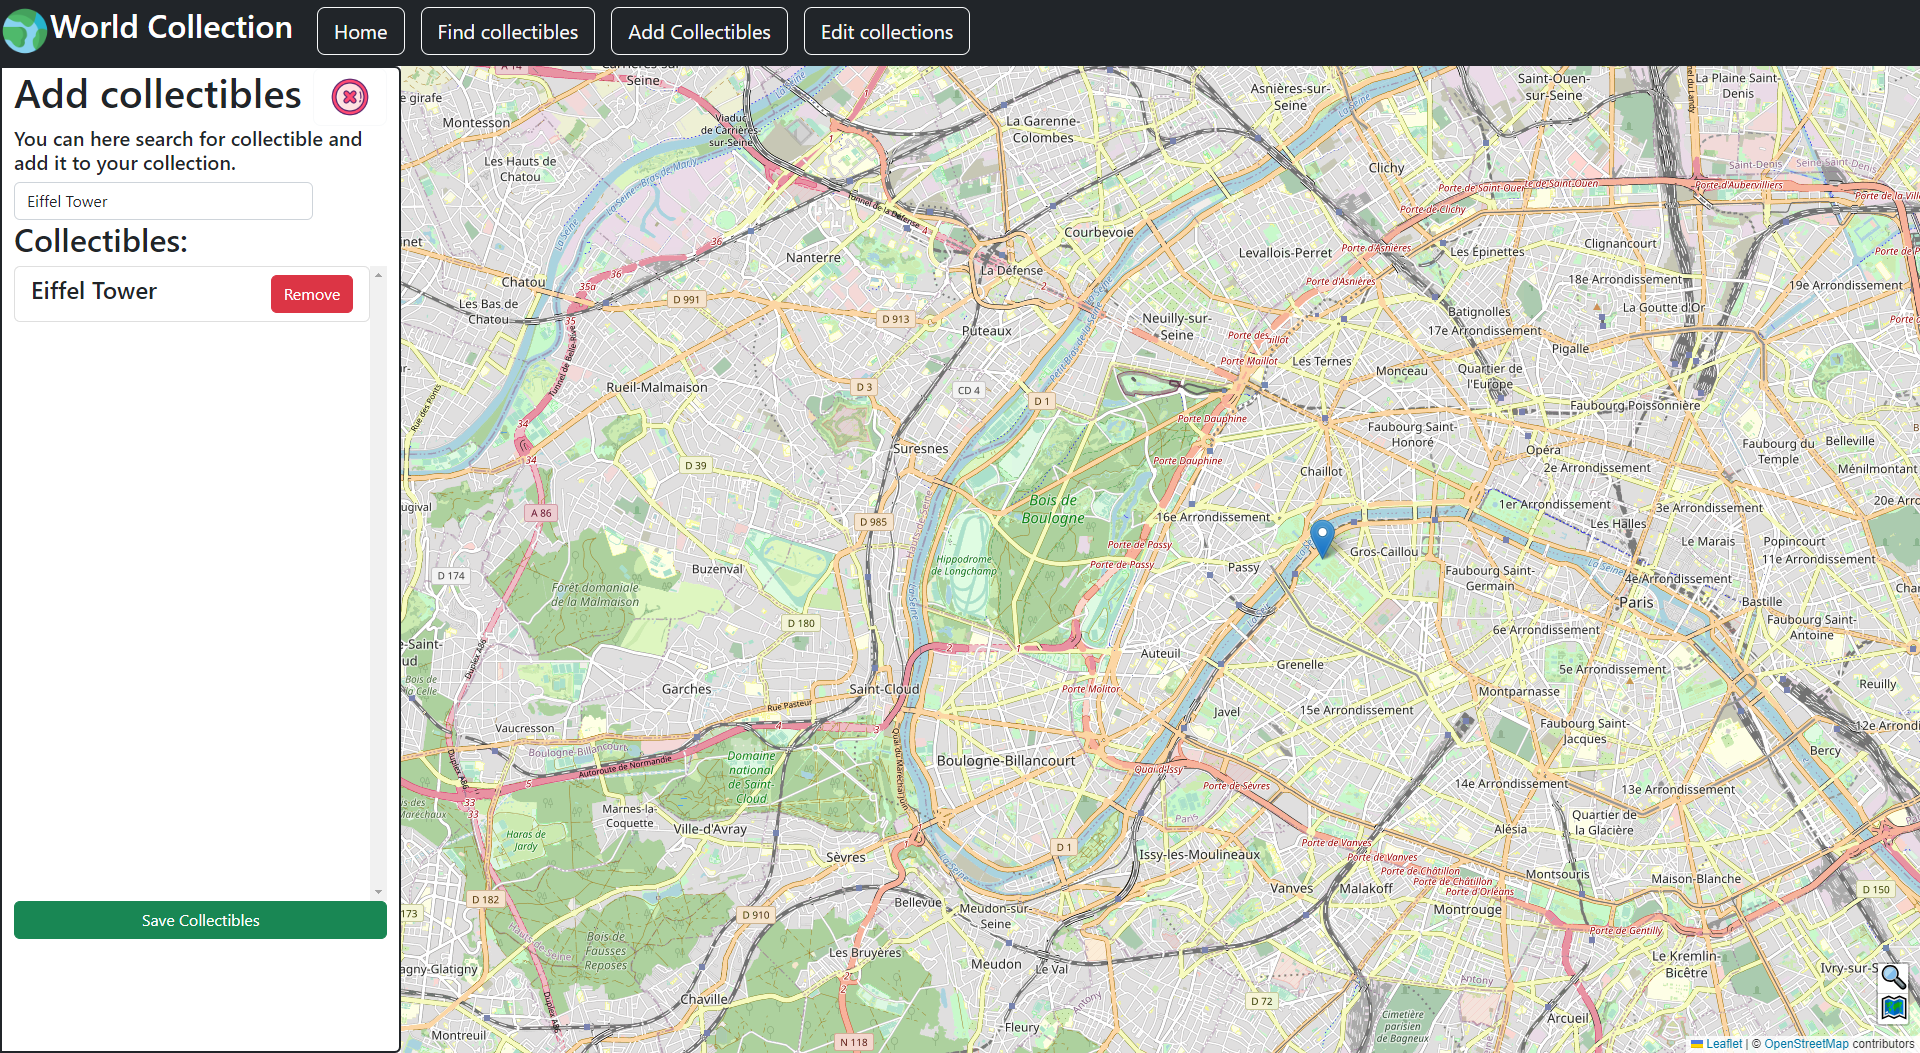
\includegraphics[width=140mm]{../img/ud-pridanie.png}
      \centering
      \caption{Ukážka pridania mapového objektu do zoznamu. }
\end{figure}

\section{Spravovanie kolekcii }

Tento stav sa zobrazí používateľovi po kliknutí tlačidla "Edit collections" v hornom navigačnom menu.

V tomto stave môže používateľ editovať svoje kolekcie a mapové objekty v nich.

Aplikácia zobrazí tabuľku, v ktorej každý riadok reprezentuje kolekciu. Kolekcie sa dajú filtrovať pomocou vstupného textového poľa.
Pre každú kolekciu tabuľka zobrazí počet mapových objektov, ktoré obsahuje a možnosť kolekciu:
\begin{itemize}
      \item zmazať - vymaže kolekciu a aj všetky mapové objekty, ktoré do nej patria
      \item spojiť - tlačidlo "Merge". Zobrazí selektor so všetkými zvyšnými kolekciami, okrem tej pre ktorú je táto možnosť zvolená. Potom ako používateľ vyberie kolekciu a stlačí tlačidlo "Merge" sa
            všetky mapové objekty kolekcie presunu do zvolenej kolekcie v selektore. Kolekcie sa spoja do kopy.
      \item editovať - zmeniť názov kolekcie, alebo zvoliť obrázok bodu pre všetky mapové objekty v kolekcii. Vhodné ak používateľ má uložené v kolekcii také mapové objekty, ktoré chce aby všetky mali rovnaký obrázok ikonky bodu.
      \item editovať mapové objekty - pomocou tlačidla "Edit Collectibles", zobrazí sa podobná tabuľka, ale teraz v nej nebudú kolekcie, ale mapové objekty zvolenej kolekcii. V tomto bode vie používateľ
            jednotlivé mapové objekty zmazať alebo meniť pomocou tlačidla "Edit" názov mapového objektu. Tlačidlom "Back to Collections" sa používateľ vráti na tabuľku s kolekciami.
\end{itemize}

\begin{figure}[h]
      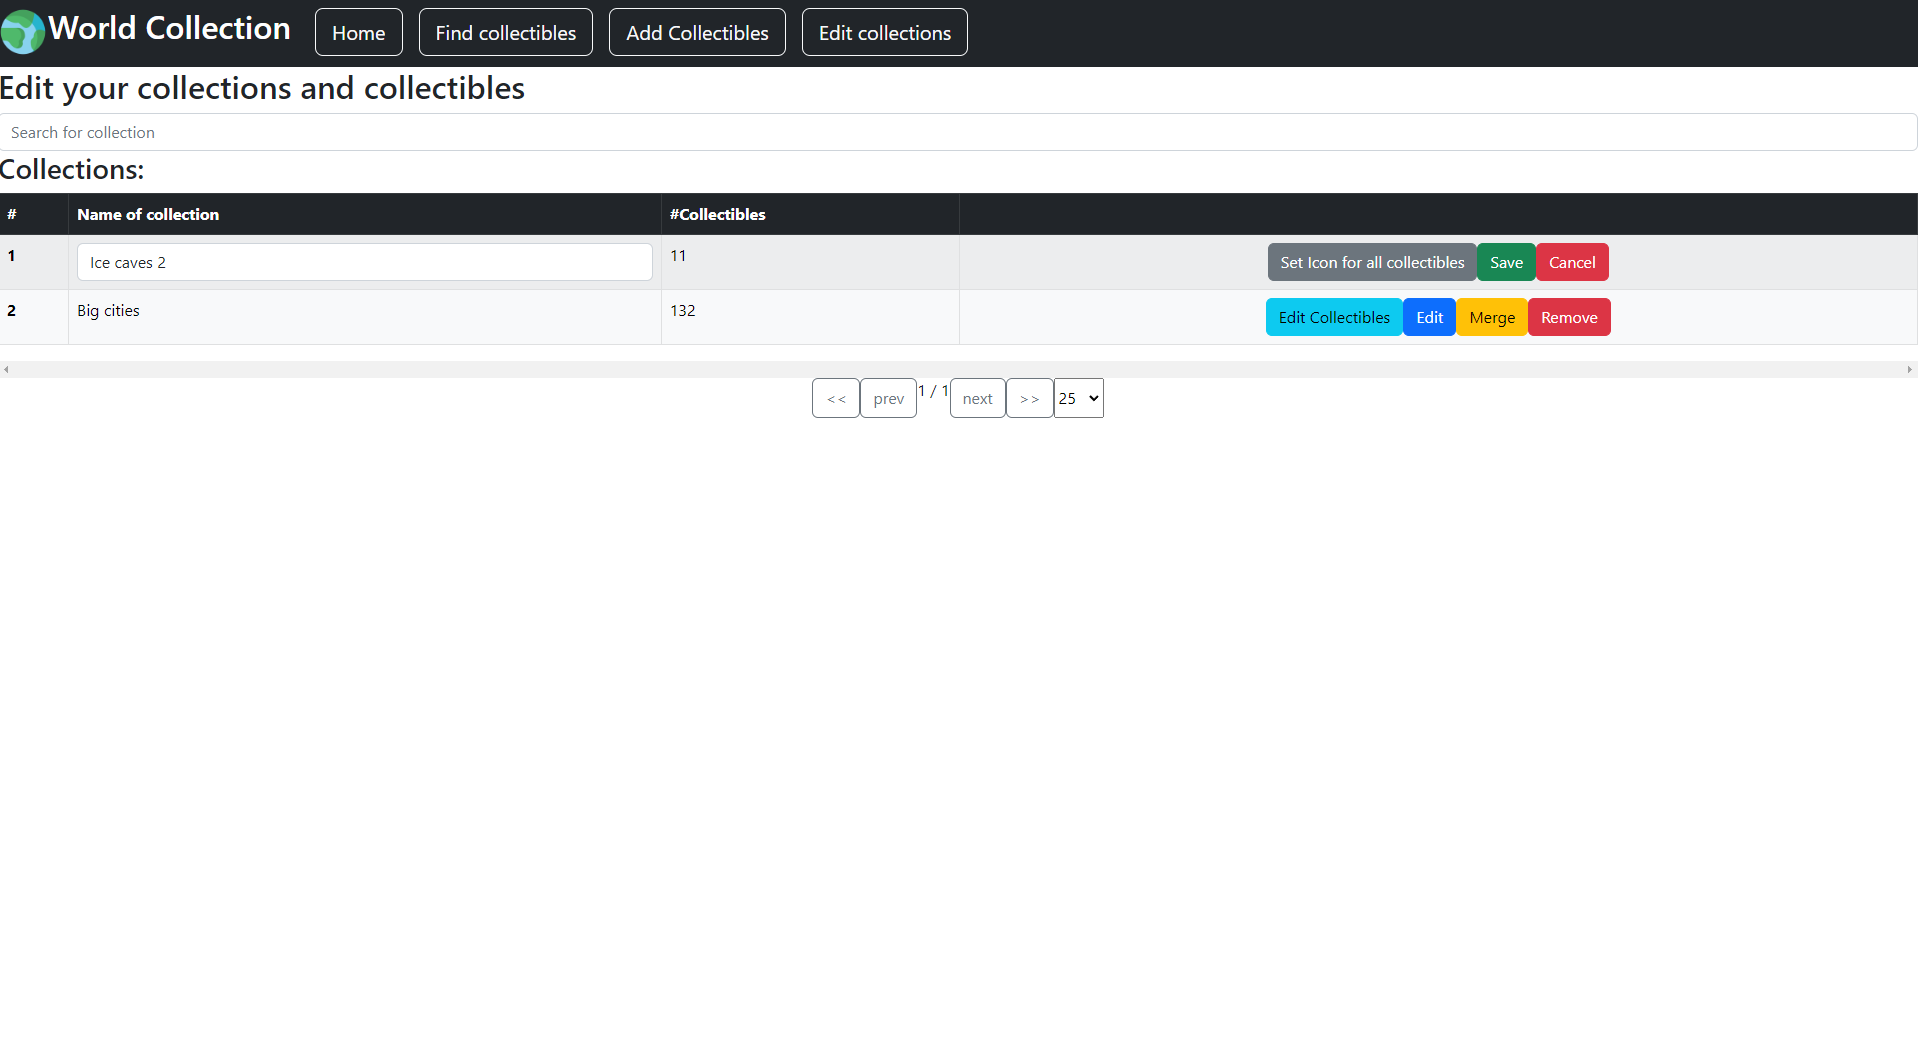
\includegraphics[width=140mm]{../img/ud-spravovanie.png}
      \centering
      \caption{Ukážka spravovania kolekcii a zmena mena kolekcie.}
\end{figure}


\chapter{Testovanie }
V tejto kapitole si popíšeme testovanie aplikácie. Nazačiatku zvolíme vhodnú technológiu na testovanie webovej aplikácie, popíšeme v krátkosti 
základ vybratej technológie, ako inštalácia a spustenie. Na záver si prejdeme testy, ktoré majú za úlohu našu aplikáciu otestovať. 

\section{Playwrig}

Pre testovanie aplikácie sme zvolili technológiu Playwrig. Jedná sa o Node.js knižnicu, ktorá podporuje moderné renderujúce nástroje ako Chromium, WebKit a Firefox. 
Knižnicu Playwrig môžeme používať v rôznych jazykov a jeden z nich je aj Typescript, v ktorom sme implementovali frontend časť aplikácie a zároveň v ním budeme písať zdrojové kódy jednotlivých testov. 
Pri testovaní sa každý test testuje izolovane od ostatných. Inak povedane sa pre každý test vytvorí novy kontext prehliadača. 

Použitím Playwrig sa vieme navigovať na rôzne URL adresy a potom na nich interagovať s elementami nachádzajúcimi sa na stránke. V našich testoch budeme simulovať používateľa, ktorý používa aplikáciu. 
V každom teste používate príde na URL. Následne so stránkou interaguje  pomocou tlačidiel a vstupných poli, do ktorých zadáva hodnoty. Všetky tieto kroky testami nasimulujeme a potom overíme či sa  
na stránke zobrazili správne elementy obsahujúce správny kontext. 

\section{Inštalácia a spustenie }
\subsection*{Inštalácia}
Playwrig sa inštaluje veľmi jedného použitím npm. V termináli z adresára  world-collection-app spustíme nasledujúci príkaz: 
\begin{code}
      npm init playwright@latest
\end{code}

Počas inštalácie si vyberieme jazyk Typescript a pomenujeme adresár, v ktorom budeme mať dokumenty obsahujúce testy. 
Po inštalácii sa nám vytvorí adresár tests a tests-examples obsahujúce základné ukážkové testy pre získanie lepšej predstavy ako sa píšu testy.  
Zároveň sa nám do dokumentu package.json pridajú závislosti potrebné na spúšťanie testy. 

\subsection*{Spustenie}
Bez zmenenia konfigurácie v dokumente playwright.config.ts sa testy budú spustené pre tri prehliadače a to chromium, firefox a WebKit. Spustené testy nám neotvoria žiadne okno v prehliadači, sú takzvane "headless". 
Výsledky testov sa nám zobrazia v termináli. 

Nasledujúcim príkazom spustime všetky testy: 
\begin{code}
      npx playwright test
\end{code}

Aby testy správne otestovali aplikáciu je potrebné aby bola spustená backend aj frontend časť aplikácie. 
V opačnom prípade testy zlyhajú. 

\subsection*{VScode rozšírenie}
Pre jednoduchšie testovanie si nainštalujeme rozšírenie “Playwright Test for VSCode” do nášho vývojového prostredia VSCode. 
Toto rozšírenie nám umožni napríklad spustiť testy jedným kľuknutím, alebo spustiť viacero testov naraz. Zároveň nám to poskytne mechanizmus na vyber lokátora v HTML dokumente, ktorým získame konkrétny element. 


\section{Playwright testy}
\subsection*{Štruktúra testov }
Všetky testy nájdeme v adresári world-collection-app/tests. V tomto adresári nájdeme päť dokumentov obsahujúcich skupinu testov a dokument MocksData.ts. 
V každom dokumente sú testy, ktoré spolu testujú jeden stav aplikácie. Naša aplikácia má štyri stavy, a preto pre každý jeden z nich vytvoríme nasledujúce dokumenty: 
\begin{itemize}
      \item Prehlaď kolekcii - collectionsOverview.spec.ts
      \item Vyhľadanie mapových objektov - findCollectibles.spec.ts
      \item Pridanie mapového objektu - addCollectible.spec.ts 
      \item Editácia - editCollections.spec.ts
\end{itemize}

V stave “Prehlaď kolekcii” môže používateľ kliknúť na bod nachádzajúci sa na interaktívnej mape. Po kliknutí na tento bod sa zobrazí “okienko” obsahujúce informácie o mapovom objekte a možnosti modifikovať poznámky a podobne. 
Správnosť tohto okienka otestujeme testami v samostatnom dokumente collectibleCard.spec. 

\subsection*{Mocks dáta}
Aby sme otestovali aplikáciu je potrebné získať dáta z backendu. Dáta poskytnuté z WikidataAPI sú v poriadku, pretože od ničoho nezávisia. Problém je ale z dátami z WorldColectionAPI. 
Tieto dáta už závisia od toho, čo je uložené v databáze. Z toho dôvodu použijeme Mock API požiadavky. 

\begin{code}
import { collectibles, collections } from "./MocksData";
//....
await page.route(
      'http://localhost:3000/WorldCollectionAPI/
      get/collections?data=%7B%7D',
      async route => {
      const json = collections;
      await route.fulfill({ json });
      }
);
//....
\end{code}
Predchádzajúca ukážka kódu sa postará o to aby počas testovania sa všetky volania na uvedený URL koncový uzol zachytili. To znamená, že skutočne volania nebudú uskutočnene  
a vrátene výsledky sa nahradia testovacími dátami.  
Testovacie dáta nájdeme v dokumente MocksData.ts. V ňom vytvoríme dve Json testovacie dáta reprezentujúce kolekcie a mapové objekty patriace do kolekcii. Tieto dve entity nám reprezentujú databázu. 

\subsection*{Štruktúra testu }
Každý jeden dokument obsahuje skupinu testov. 
V tejto skupine vytvoríme konkrétne testy. Každý test berie ako argument názov testu a testovaciu funkciu. Tato funkcia berie jeden argument a to takzvaný objekt "page" reprezentujúci jednoducho povedané webovú stránku. 

Aby sme nemuseli pred každým testom vykonávať tu istú činnosť tak využijeme možnosť definovať v skupine testov aj test “tests.beforeEach”. Tento test sa automaticky spusti pred každým jedným testov patriacim do skupiny testov. 
V tomto teste nastavíme Mock API požiadavky, aby sme dostavali testovacie dáta namiesto dát z databázy. Zároveň dostaneme stránku do stavu v akom sa pred každým testom bude nachládať. 

V nasledujúcej ukážke si ukážeme jeden test: 
\begin{code}
test.describe("collection overview tests", () => {
test.beforeEach(async ({ page }) => {
// Mock API requests
// collections
await page.route('http://localhost:3000/WorldCollectionAPI/
      get/collections?data=%7B%7D', async route => {
      const json =
            collections
      ;
      await route.fulfill({ json });
      });
      // collectibles
      await page.route('http://localhost:3000/WorldCollectionAPI/
      get/collectibles?data=%7B%22collectionID%22%3A1%7D', async route => {
      const json =
            collectibles
            ;
      await route.fulfill({ json });
      });
      await page.goto('http://localhost:3000/');
})

test("open and close list of collections", async ({ page }) => {
      await expect(page.getByTestId('collectionsMenu')).not.toBeVisible()
      await page.getByTestId('buttonToOpenCollectionList').click();
      await expect(page.getByTestId('collectionsMenu')).toBeVisible()
      await page.getByTestId('close collectionsMenu').click();
      await expect(page.getByTestId('collectionsMenu')).not.toBeVisible()
});
\end{code}
Tento test otestuje funkčnosť širšieho bočného panelu vo stave "Prehlaď kolekcii", či dôkaze používateľ otvoriť a následne zatvoriť tento panel. 


Aby sme mohli pracovať s elementami, tak je potrebne ich najprv nájsť v objekte “page”. Pre výber môžeme použiť viacero spôsobov. 
Jeden z nich je použitý v ukážke kódu. Funkcia page.getByTestId() nám vráti element, ktorý obsahuje “data-testid”. 

Nasledujuca ukážka ukazuje tento element ako je označený v zdrojovom kóde:
\begin{code}
      <button data-testid="buttonToOpenCollectionList" ... </button>
\end{code}

V testoch často krát testujeme, či je konkrétny element viditeľní, alebo naopak neviditeľní. To môžeme vidieť aj v ukážke vyššie. Najprv otestujeme, že širší panel nie je zobrazení, 
po kliknutí správneho tlačidla sa tento panel zobrazí a následne kliknutím iného tlačidla sa znovu nezobrazí. 

\section{Prehlaď testov}

V tejto sekcii si v krátkosti popíšeme funkciu skupiny testov v jedovlivých dokumentov, čo testy v nich majú za úlohu otestovať. 
Testy pokrývajú iba najdôležitejšiu časť aplikácie. Aby sme otestovali úplne všetko je potrebné napísať viacej testov.ň
Pre túto prácu nám to príde nie, až tak podstatné.

\subsection*{collectionsOverview.spec}
Testy nachádzajúce sa v tomto dokumente majú za úlohu otestovať funkčnosť bočného panelu. 
Tým myslime, že jeden test otestuje či je možné tento panel otvoriť a zároveň aj zatvoriť. Ďalej či je v panely správne vykreslený zoznam obsahujúci informácie o kolekciách. 
Funkčnosť vstupného poľa, ktoré sa nachláda v tomto panely. Potom ako do neho používateľ uvedie názov kolekcie, tak sa zobrazí v zozname iba táto kolekcia. 
Posledným testom otestujeme, či po sa kliknutí na bod zobrazí na stránke “okienko” obsahujúce informácie. 

\subsection*{collectibleCard.spec}
Týmito testami otestujeme vyššie spomenuté okienko.  
Nájdeme tu testy testujúce jednotlivé elementy ako zobrazenie obrázku, informácii o mapovom objekte a tlačidlá, ktoré po kliknutí vykreslia správne elementy. 

\subsection*{addCollectible.spec}
Nájdeme tu testy, ktoré otestujú funkčnosť vyhľadávania mapového objektu, jeho pridávania do a zmazania zo zoznamu. 
Zároveň je tu jeden test na otestovanie bočného panelu. Ten sa otestuje rovnakým princípom ako bol test v collectionsOverview.spec. 

\subsection*{findCollectibles.spec}
V tejto skupine testov nájdeme tri testy. Každý jeden z nich ma za úlohu otestovať jeden krok zadávania parametrov počas procesu vyhľadávania skupiny mapových objektov na základe parametrov. 
V prvom teste otestujeme výber kategórie. Nasimulujeme, že používateľ zadá názov kategórie do vyhľadávacieho poľa a následne vyberie hľadanú kategóriu. 
Týmto otestujeme aj WikidataAPI, čí správne funguje a vracajú správny výsledok. 

V druhom teste zvolíme vyber oblasti a zadáme oblasť. V poslednom teste otestujeme vybratie filtra z ponúknutých možnosti a následne zvolenie hodnoty tohto filtra. 

Testy netestujú všetky možnosti. V každom kroku sa zvoli iba jedna. 

\subsection*{editCollections.spec}
Nájdeme tu dva testy. Jeden nám otestuje, či sa nám správne zobrazí editačná tabuľka pre kolekcie, obsahujúca testovacie dáta, ktoré reprezentujú kolekcie. 
Či informácie v nej sa správne zobrazene a zároveň, či sa zobrazia aj tlačidla reprezentujúce upravovanie kolekcii. 

V druhom otestujeme podobným princípom editačnú tabuľku mapových objektov, ktorá sa ma zobrazí potom ako používateľ klikne na správne tlačidlo nachádzajúce sa v prvej editačnej tabuľke. 

%%% Fiktivní kapitola s ukázkami tabulek, obrázků a kódu
\chapter{Ukáźky}
Vlastní text bakalářské práce je uspořádaný hierarchicky do kapitol a podkapitol,
každá kapitola začíná na nové straně. Text je zarovnán do bloku. Nový odstavec
se obvykle odděluje malou vertikální mezerou a odsazením prvního řádku. Grafická
úprava má být v~celém textu jednotná.

Práce se tiskne na bílý papír formátu A4. Okraje musí ponechat dost místa na vazbu:
doporučen je horní, dolní a pravý okraj $25\,\rm mm$, levý okraj $40\,\rm mm$.
Číslují se všechny strany kromě obálky a informačních stran na začátku práce;
první číslovaná strana bývá obvykle ta s~obsahem.

Písmo se doporučuje dvanáctibodové ($12\,\rm pt$) se standardní vzdáleností mezi řádky
(pokud píšete ve Wordu nebo podobném programu, odpovídá tomu řádkování $1,5$; v~\TeX{}u
není potřeba nic přepínat). Pro běžný text používejte vzpřímené patkové písmo.
Text matematických vět se obvykle tiskne pro zdůraznění skloněným (slanted) písmem,
není-li k~dispozici, může být zastoupeno kurzívou.

Primárně je doporučován jednostranný tisk (příliš tenkou práci lze obtížně svázat).
Delší práce je lepší tisknout oboustranně a přizpůsobit tomu velikosti okrajů:
$40\,\rm mm$ má vždy \emph{vnitřní} okraj. Rub titulního listu zůstává nepotištěný.

Zkratky použité v textu musí být vysvětleny vždy u prvního výskytu zkratky (v~závorce nebo
v poznámce pod čarou, jde-li o složitější vysvětlení pojmu či zkratky). Pokud je zkratek
více, připojuje se seznam použitých zkratek, včetně jejich vysvětlení a/nebo odkazů
na definici.

Delší převzatý text jiného autora je nutné vymezit uvozovkami nebo jinak vyznačit a řádně
citovat.

\section{Jednoduché příklady}

Čísla v~českém textu obvykle sázíme v~matematickém režimu s~desetinnou čárkou:
%%% Bez \usepackage{icomma}:
% $\pi \doteq 3{,}141\,592\,653\,589$.
%%% S \usepackage{icomma}:
$\pi \doteq 3,141\,592\,653\,589$.
V~matematických textech se považuje za přípustné používat desetinnou tečku
(pro lepší odlišení od čárky v~roli oddělovače). Numerické výsledky se uvádějí
s~přiměřeným počtem desetinných míst.

Mezi číslo a jednotku patří úzká mezera: šířka stránky A4 činí $210\,\rm mm$, což si
pamatuje pouze $5\,\%$ autorů. Pokud ale údaj slouží jako přívlastek, mezeru vynecháváme:
$25\rm mm$ okraj, $95\%$ interval spolehlivosti.

Rozlišujeme různé druhy pomlček:
červeno-černý (krátká pomlčka),
strana 16--22 (střední),
$45-44$ (matematické minus),
a~toto je --- jak se asi dalo čekat --- vložená věta ohraničená dlouhými pomlčkami.

V~českém textu se používají \uv{české} uvozovky, nikoliv ``anglické''.

% V tomto odstavci se vlnka zviditelňuje
{
\def~{{\tt\char126}}
Na některých místech je potřeba zabránit lámání řádku (v~\TeX{}u značíme vlnovkou):
u~předložek (neslabičnych, nebo obecně jednopísmenných), vrchol~$v$, před $k$~kroky,
a~proto, \dots{} obecně kdekoliv, kde by při rozlomení čtenář \uv{ško\-brt\-nul}.
}

\section{Matematické vzorce a výrazy}

Proměnné sázíme kurzívou (to \TeX{} v~matematickém módu dělá sám, ale
nezapomínejte na to v~okolním textu a také si matematický mód zapněte).
Názvy funkcí sázíme vzpřímeně. Tedy například:
$\var(X) = \E X^2 - \bigl(\E X \bigr)^2$.

Zlomky uvnitř odstavce (třeba $\frac{5}{7}$ nebo $\frac{x+y}{2}$) mohou
být příliš stísněné, takže je lepší sázet jednoduché zlomky s~lomítkem:
$5/7$, $(x+y)/2$.

Nechť
\[   % LaTeXová náhrada klasického TeXového $$
      \mathbb{X} = \begin{pmatrix}
            \T{\bm x_1} \\
            \vdots      \\
            \T{\bm x_n}
      \end{pmatrix}.
\]
Povšimněme si tečky za~maticí. Byť je matematický text vysázen
ve~specifickém prostředí, stále je gramaticky součástí věty a~tudíž je
zapotřebí neopomenout patřičná interpunkční znaménka. Výrazy, na které
chceme později odkazovat, je vhodné očíslovat:
\begin{equation}\label{eq01:Xmat}
      \mathbb{X} = \begin{pmatrix}
            \T{\bm x_1} \\
            \vdots      \\
            \T{\bm x_n}
      \end{pmatrix}.
\end{equation}
Výraz \eqref{eq01:Xmat} definuje matici $\mathbb{X}$. Pro lepší čitelnost
a~přehlednost textu je vhodné číslovat pouze ty výrazy, na které se
autor někde v~další části textu odkazuje. To jest, nečíslujte
automaticky všechny výrazy vysázené některým z~matematických
prostředí.

Zarovnání vzorců do několika sloupečků:
\begin{alignat*}{3}
      S(t) & = \pr(T > t),    & \qquad t & >0 & \qquad & \text{ (zprava spojitá),} \\
      F(t) & = \pr(T \leq t), & \qquad t & >0 & \qquad & \text{ (zprava spojitá).}
\end{alignat*}

Dva vzorce se spojovníkem:
\begin{equation}\label{eq01:FS}
      \left.
      \begin{aligned}
            S(t) & = \pr(T > t)    \\[1ex]
            F(t) & = \pr(T \leq t)
      \end{aligned}
      \;	% zde pomůže ručně vynechat trochu místa
      \right\}
      \quad t>0 \qquad \text{(zprava spojité).}
\end{equation}

Dva centrované nečíslované vzorce:
\begin{gather*}
      \bm Y = \mathbb{X}\bm\beta + \bm\varepsilon, \\[1ex]
      \mathbb{X} = \begin{pmatrix} 1 & \T{\bm x_1} \\ \vdots & \vdots \\ 1 &
                \T{\bm x_n}\end{pmatrix}.
\end{gather*}
Dva centrované číslované vzorce:
\begin{gather}
      \bm Y = \mathbb{X}\bm\beta + \bm\varepsilon, \label{eq02:Y}\\[1ex]
      \mathbb{X} = \begin{pmatrix} 1 & \T{\bm x_1} \label{eq03:X} \\ \vdots & \vdots \\ 1 &
                \T{\bm x_n}\end{pmatrix}.
\end{gather}

Definice rozdělená na dva případy:
\[
      P_{r-j}=
      \begin{cases}
            0,                  & \text{je-li $r-j$ liché}, \\
            r!\,(-1)^{(r-j)/2}, & \text{je-li $r-j$ sudé}.
      \end{cases}
\]
Všimněte si použití interpunkce v této konstrukci. Čárky a tečky se
dávají na místa, kam podle jazykových pravidel patří.

\begin{align}
      x & = y_1-y_2+y_3-y_5+y_8-\dots = &  & \text{z \eqref{eq02:Y}} \nonumber     \\
        & = y'\circ y^* =               &  & \text{podle \eqref{eq03:X}} \nonumber \\
        & = y(0) y'                     &  & \text {z Axiomu 1.}
\end{align}


Dva zarovnané vzorce nečíslované:
\begin{align*}
      L(\bm\theta)    & = \prod_{i=1}^n f_i(y_i;\,\bm\theta), \\
      \ell(\bm\theta) & = \log\bigl\{L(\bm\theta)\bigr\} =
      \sum_{i=1}^n \log\bigl\{f_i(y_i;\,\bm\theta)\bigr\}.
\end{align*}
Dva zarovnané vzorce, první číslovaný:
\begin{align}
      L(\bm\theta)    & = \prod_{i=1}^n f_i(y_i;\,\bm\theta), \label{eq01:L} \\
      \ell(\bm\theta) & = \log\bigl\{L(\bm\theta)\bigr\} =
      \sum_{i=1}^n \log\bigl\{f_i(y_i;\,\bm\theta)\bigr\}. \nonumber
\end{align}

Vzorec na dva řádky, první řádek zarovnaný vlevo, druhý vpravo, nečíslovaný:
\begin{multline*}
      \ell(\mu,\,\sigma^2) = \log\bigl\{L(\mu,\,\sigma^2)\bigr\} =
      \sum_{i=1}^n \log\bigl\{f_i(y_i;\,\mu,\,\sigma^2)\bigr\}= \\
      = -\,\frac{n}{2}\,\log(2\pi\sigma^2) \,-\,
      \frac{1}{2\sigma^2}\sum_{i=1}^n\,(y_i - \mu)^2.
\end{multline*}

Vzorec na dva řádky, zarovnaný na $=$, číslovaný uprostřed:
\begin{equation}\label{eq01:ell}
      \begin{split}
            \ell(\mu,\,\sigma^2) &= \log\bigl\{L(\mu,\,\sigma^2)\bigr\} =
            \sum_{i=1}^n \log\bigl\{f(y_i;\,\mu,\,\sigma^2)\bigr\}= \\
            & = -\,\frac{n}{2}\,\log(2\pi\sigma^2) \,-\,
            \frac{1}{2\sigma^2}\sum_{i=1}^n\,(y_i - \mu)^2.
      \end{split}
\end{equation}

\section{Definice, věty, důkazy, \dots}

Konstrukce typu definice, věta, důkaz, příklad, \dots je vhodné
odlišit od okolního textu a~případně též číslovat s~možností použití
křížových odkazů. Pro každý typ těchto konstrukcí je vhodné mít
v~souboru s~makry (\texttt{makra.tex}) nadefinované jedno prostředí,
které zajistí jak vizuální odlišení od okolního textu, tak
automatické číslování s~možností křížově odkazovat.

\begin{definice}\label{def01:1}
      Nechť náhodné veličiny $X_1,\dots,X_n$ jsou definovány na témž
      prav\-dě\-po\-dob\-nost\-ním prostoru $(\Omega,\,\mathcal{A},\,\pr)$. Pak
      vektor $\bm X = \T{(X_1,\dots,X_n)}$ nazveme \emph{náhodným
            vektorem}.
\end{definice}

\begin{definice}[náhodný vektor]\label{def01:2}
      Nechť náhodné veličiny $X_1,\dots,X_n$ jsou definovány na témž
      pravděpodobnostním prostoru $(\Omega,\,\mathcal{A},\,\pr)$. Pak
      vektor $\bm X = \T{(X_1,\dots,X_n)}$ nazveme \emph{náhodným
            vektorem}.
\end{definice}
Definice~\ref{def01:1} ukazuje použití prostředí pro sazbu definice
bez titulku, definice~\ref{def01:2} ukazuje použití prostředí pro
sazbu definice s~titulkem.

\begin{veta}\label{veta01:1}
      Náhodný vektor $\bm X$ je měřitelné zobrazení prostoru
      $(\Omega,\,\mathcal{A},\,\pr)$ do $(\R_n,\,\mathcal{B}_n)$.
\end{veta}

\begin{lemma}[\citealp{Andel07}, str. 29]\label{veta01:2}
      Náhodný vektor $\bm X$ je měřitelné zobrazení prostoru
      $(\Omega,\,\mathcal{A},\,\pr)$ do $(\R_n,\,\mathcal{B}_n)$.
\end{lemma}
\begin{dukaz}
      Jednotlivé kroky důkazu jsou podrobně popsány v~práci \citet[str.
            29]{Andel07}.
\end{dukaz}
Věta~\ref{veta01:1} ukazuje použití prostředí pro sazbu matematické
věty bez titulku, lemma~\ref{veta01:2} ukazuje použití prostředí pro
sazbu matematické věty s~titulkem. Lemmata byla zavedena v~hlavním
souboru tak, že sdílejí číslování s~větami.

\chapter{Tabulky, obrázky, programy}

Používání tabulek a grafů v~odborném textu má některá společná
pravidla a~některá specifická. Tabulky a grafy neuvádíme přímo do
textu, ale umístíme je buď na samostatné stránky nebo na vyhrazené
místo v~horní nebo dolní části běžných stránek. \LaTeX\ se o~umístění
plovoucích grafů a tabulek postará automaticky.

Každý graf a tabulku
očíslujeme a umístíme pod ně legendu. Legenda má popisovat obsah grafu
či tabulky tak podrobně, aby jim čtenář rozuměl bez důkladného
studování textu práce.

Na každou tabulku a graf musí být v~textu odkaz
pomocí jejich čísla. Na příslušném místě textu pak shrneme ty
nejdůležitější závěry, které lze z~tabulky či grafu učinit. Text by
měl být čitelný a srozumitelný i~bez prohlížení tabulek a grafů a
tabulky a grafy by měly být srozumitelné i~bez podrobné četby textu.

Na tabulky a grafy odkazujeme pokud možno nepřímo v~průběhu běžného
toku textu; místo \emph{\uv{Tabulka~\ref{tab03:Nejaka} ukazuje, že
            muži jsou v~průměru o~$9,9\,\rm kg$ těžší než ženy}} raději napíšeme
\emph{\uv{Muži jsou o~$9,9\,\rm kg$ těžší než ženy (viz
            Tabulka~\ref{tab03:Nejaka})}}.

\section{Tabulky}

\begin{table}[b!]

      \centering
      %%% Tabulka používá následující balíčky:
      %%%   - booktabs (\toprule, \midrule, \bottomrule)
      %%%   - dcolumn (typ sloupce D: vycentrovaná čísla zarovnaná na
      %%%     desetinnou čárku
      %%%     Všimněte si, že ve zdrojovém kódu jsou desetinné tečky, ale
      %%%     tisknou se čárky.
      %%% Dále používáme příkazy \pulrad a \mc definované v makra.tex

      \begin{tabular}{l@{\hspace{1.5cm}}D{.}{,}{3.2}D{.}{,}{1.2}D{.}{,}{2.3}}
            \toprule
                                    & \mc{}                        & \mc{\textbf{Směrod.}}   & \mc{}    \\
            \pulrad{\textbf{Efekt}} & \mc{\pulrad{\textbf{Odhad}}} & \mc{\textbf{chyba}$^a$} &
            \mc{\pulrad{\textbf{P-hodnota}}}                                                            \\
            \midrule
            Abs. člen               & -10.01                       & 1.01                    & \mc{---} \\
            Pohlaví (muž)           & 9.89                         & 5.98                    & 0.098    \\
            Výška (cm)              & 0.78                         & 0.12                    & <0.001   \\
            \bottomrule
            \multicolumn{4}{l}{\footnotesize \textit{Pozn:}
                  $^a$ Směrodatná chyba odhadu metodou Monte Carlo.}
      \end{tabular}

      \caption{Maximálně věrohodné odhady v~modelu M.}\label{tab03:Nejaka}

\end{table}

U~\textbf{tabulek} se doporučuje dodržovat následující pravidla:

\begin{itemize} %% nebo compactitem z balíku paralist
      \item Vyhýbat se svislým linkám. Silnějšími vodorovnými linkami
            oddělit tabulku od okolního textu včetně legendy, slabšími
            vodorovnými linkami oddělovat záhlaví sloupců od těla tabulky a
            jednotlivé části tabulky mezi sebou. V~\LaTeX u tuto podobu tabulek
            implementuje balík \texttt{booktabs}. Chceme-li výrazněji oddělit
            některé sloupce od jiných, vložíme mezi ně větší mezeru.
      \item Neměnit typ, formát a význam obsahu políček v~tomtéž sloupci
            (není dobré do téhož sloupce zapisovat tu průměr, onde procenta).
      \item Neopakovat tentýž obsah políček mnohokrát za sebou. Máme-li
            sloupec \textit{Rozptyl}, který v~prvních deseti řádcích obsahuje
            hodnotu $0,5$ a v~druhých deseti řádcích hodnotu $1,5$, pak tento
            sloupec raději zrušíme a vyřešíme to jinak. Například můžeme tabulku
            rozdělit na dvě nebo do ní vložit popisné řádky, které informují
            o~nějaké proměnné hodnotě opakující se v~následujícím oddíle tabulky
            (např. \emph{\uv{Rozptyl${}=0,5$}} a níže \emph{\uv{Rozptyl${}=
                              1,5$}}).
      \item Čísla v~tabulce zarovnávat na desetinnou čárku.
      \item V~tabulce je někdy potřebné používat zkratky, které se jinde
            nevyskytují. Tyto zkratky můžeme vysvětlit v~legendě nebo
            v~poznámkách pod tabulkou. Poznámky pod tabulkou můžeme využít i
            k~podrobnějšímu vysvětlení významu  některých sloupců nebo hodnot.
\end{itemize}

\section{Obrázky}

Několik rad týkajících se obrázků a grafů.

\begin{itemize}
      \item Graf by měl být vytvořen ve velikosti, v~níž bude použit
            v~práci. Zmenšení příliš velkého grafu vede ke špatné čitelnosti
            popisků.
      \item Osy grafu musí být řádně popsány ve stejném jazyce, v~jakém je
            psána práce (absenci diakritiky lze tolerovat). Kreslíme-li graf
            hmotnosti proti výšce, nenecháme na nich popisky \texttt{ht} a
            \texttt{wt}, ale osy popíšeme \emph{Výška [cm]} a~\emph{Hmotnost
                        [kg]}. Kreslíme-li graf funkce $h(x)$, popíšeme osy $x$ a $h(x)$.
            Každá osa musí mít jasně určenou škálu.
      \item Chceme-li na dvourozměrném grafu vyznačit velké množství bodů,
            dáme pozor, aby se neslily do jednolité černé tmy. Je-li bodů mnoho,
            zmenšíme velikost symbolu, kterým je vykreslujeme, anebo vybereme
            jen malou část bodů, kterou do grafu zaneseme. Grafy, které obsahují
            tisíce bodů, dělají problémy hlavně v~elektronických dokumentech,
            protože výrazně zvětšují velikost souborů.
      \item Budeme-li práci tisknout černobíle, vyhneme se používání barev.
            Čáry roz\-li\-šu\-je\-me typem (plná, tečkovaná, čerchovaná,\ldots), plochy
            dostatečně roz\-díl\-ný\-mi intensitami šedé nebo šrafováním. Význam
            jednotlivých typů čar a~ploch vysvětlíme buď v~textové legendě ke
            grafu anebo v~grafické legendě, která je přímo součástí obrázku.
      \item Vyhýbejte se bitmapovým obrázkům o~nízkém rozlišení a zejména
            JPEGům (zuby a kompresní artefakty nevypadají na papíře pěkně).
            Lepší je vytvářet obrázky vektorově a vložit do textu jako PDF.
\end{itemize}

\section{Programy}

Algoritmy, výpisy programů a popis interakce s~programy je vhodné
odlišit od ostatního textu. Jednou z~možností je použití {\LaTeX}o\-vé\-ho balíčku
\texttt{fancyvrb} (fancy verbatim), pomocí něhož je v~souboru \texttt{makra.tex}
nadefinováno prostředí \texttt{code}. Pomocí něho lze vytvořit
např. následující ukázky.

\begin{code}
      > mean(x)
      [1] 158.90
      > objekt$prumer
            [1] 158.90
\end{code}
%$
Menší písmo:
\begin{code}[fontsize=\footnotesize]
      > mean(x)
      [1] 158.90
      > objekt$prumer
            [1] 158.90
\end{code}
%$
Bez rámečku:
\begin{code}[frame=none]
      > mean(x)
      [1] 158.90
      > objekt$prumer
            [1] 158.90
\end{code}
%$
Užší rámeček:
\begin{code}[xrightmargin=20em]
      > mean(x)
      [1] 158.90
      > objekt$prumer
            [1] 158.90
\end{code}
%$

\begin{figure}[p]\centering
      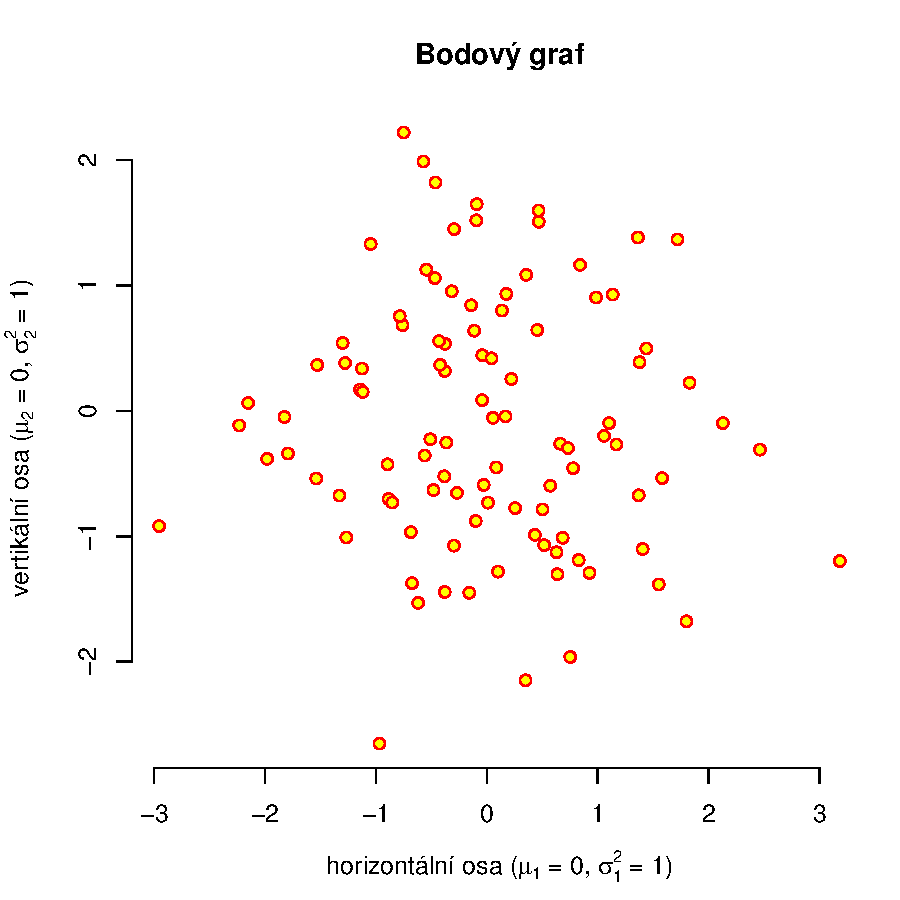
\includegraphics[width=140mm, height=140mm]{../img/ukazka-obr01}
      % Příponu není potřeba explicitně uvádět, pdflatex automaticky hledá pdf.
      % Rozměry také není nutné uvádět.
      \caption{Náhodný výběr z~rozdělení $\mathcal{N}_2(\boldsymbol{0},\,I)$.}
      \label{obr03:Nvyber}

\end{figure}

\begin{figure}[p]\centering
      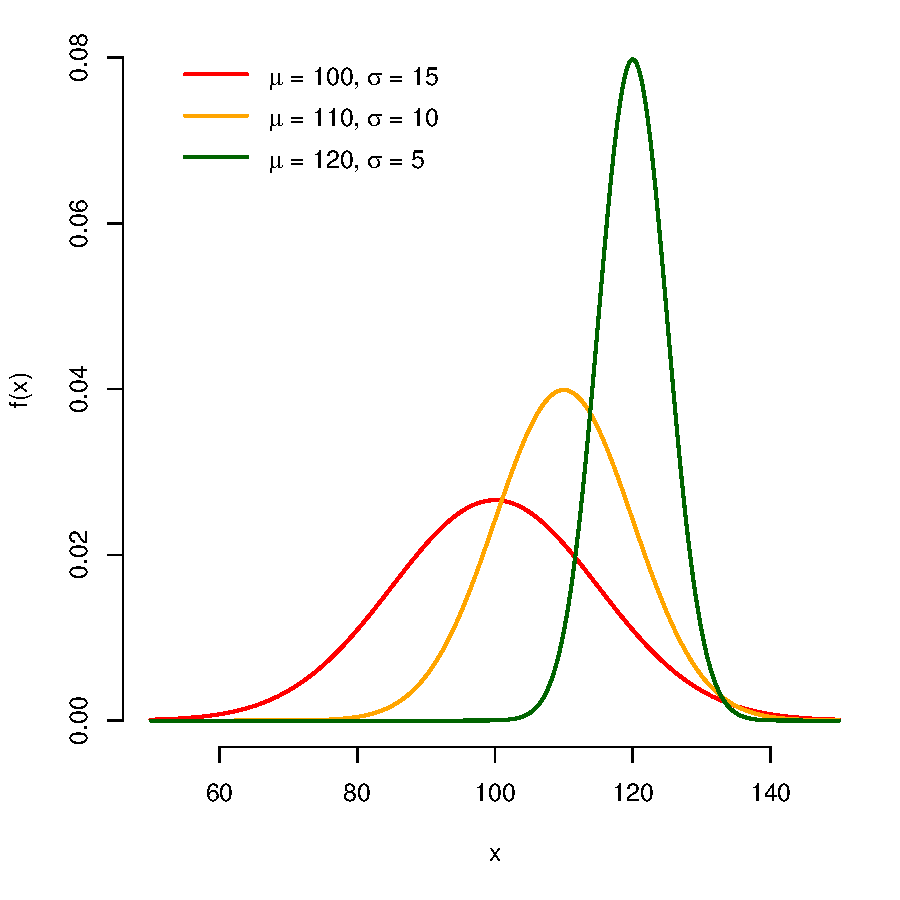
\includegraphics[width=140mm, height=140mm]{../img/ukazka-obr02}
      \caption{Hustoty několika normálních rozdělení.}
      \label{obr03:Nhust}
\end{figure}

\begin{figure}[p]\centering
      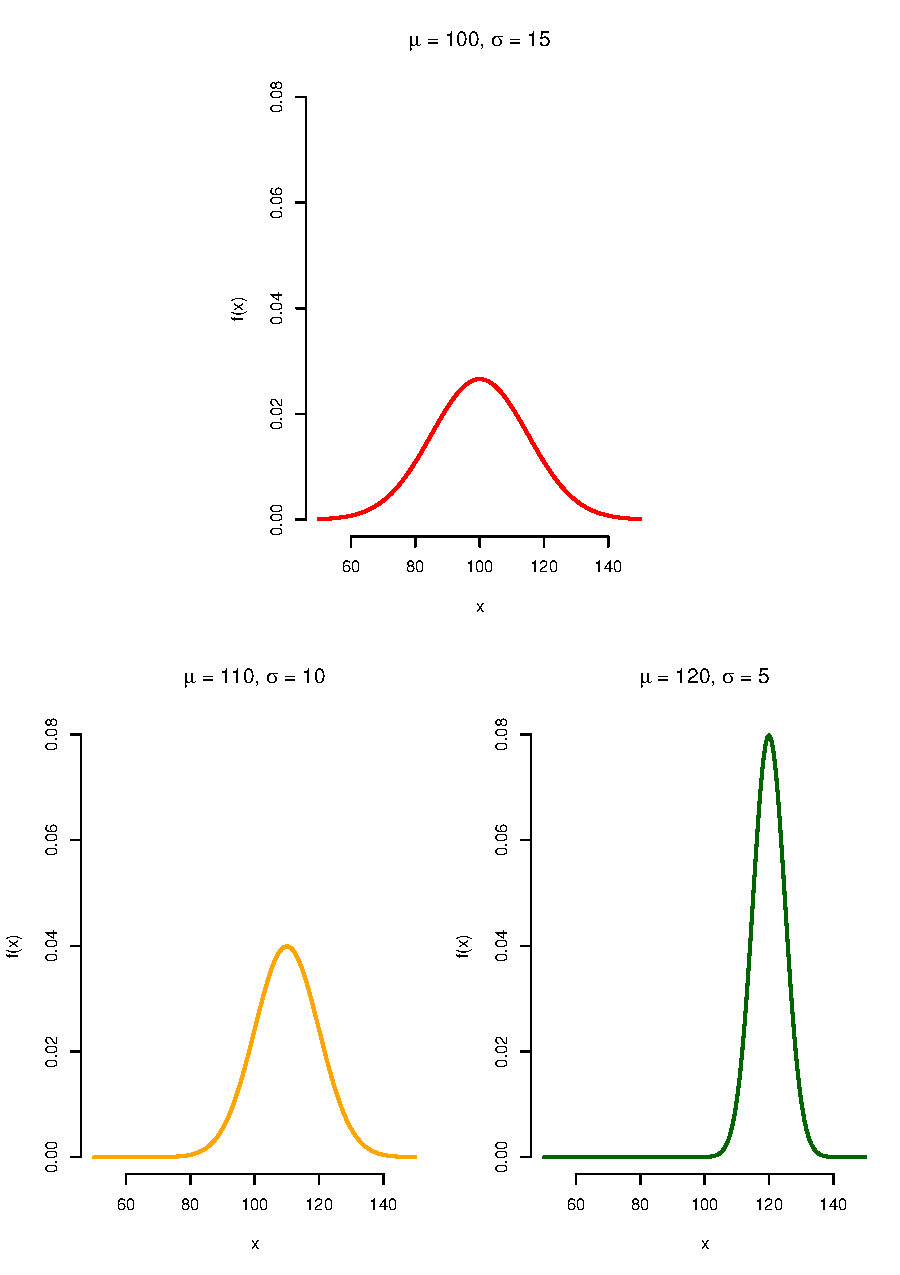
\includegraphics[width=140mm, height=198mm]{../img/ukazka-obr03}
      \caption{Hustoty několika normálních rozdělení.}
      \label{obr03:Nhust:podruhe}

\end{figure}

\chapter{Odkazy na literaturu}

Odkazy na literaturu vytváříme nejlépe pomocí příkazů
\verb|\citet|, \verb|\citep| atp.
(viz {\LaTeX}ový balíček \textsf{natbib}) a~následného použití
Bib{\TeX}u. V~matematickém textu obvykle odkazujeme stylem \uv{Jméno
      autora/autorů (rok vydání)}, resp. \uv{Jméno autora/autorů [číslo
odkazu]}. V~českém/slovenském textu je potřeba se navíc vypořádat
s~nutností skloňovat jméno autora, respektive přechylovat jméno
autorky. Je potřeba mít na paměti, že standardní příkazy
\verb|\citet|, \verb|\citep|
produkují referenci se jménem autora/autorů v~prvním pádě a~jména
autorek jsou nepřechýlena.

Pokud nepoužíváme bib\TeX{}, řídíme se normou ISO 690 a zvyklostmi
oboru.

Jména časopisů lze uvádět zkráceně, ale pouze v~kodifikované podobě.

\section{Několik ukázek}

Mezi nejvíce citované statistické články patří práce Kaplana a~Meiera a~Coxe
\citep{KaplanMeier58, Cox72}. \citet{Student08} napsal článek o~t-testu.

Prof. Anděl je autorem učebnice matematické statistiky
\citep[viz][]{Andel98}. Teorii odhadu se věnuje práce
\citet{LehmannCasella98}. V~případě odkazů na specifickou informaci
(definice, důkaz, \dots) uvedenou v~knize bývá užitečné uvést
specificky číslo kapitoly, číslo věty atp. obsahující požadovanou
informaci, např. viz \citet[Věta 4.22]{Andel07} nebo \citep[viz][Věta
      4.22]{Andel07}.

Mnoho článků je výsledkem spolupráce celé řady osob. Při odkazování
v~textu na článek se třemi autory obvykle při prvním výskytu uvedeme
plný seznam: \citet*{DempsterLairdRubin77} představili koncept EM
algoritmu. Respektive: Koncept EM algoritmu byl představen v~práci
Dempstera, Lairdové a~Rubina \citep*{DempsterLairdRubin77}. Při každém
dalším výskytu již používáme zkrácenou verzi:
\citet{DempsterLairdRubin77} nabízejí též několik příkladů použití EM
algoritmu. Respektive: Několik příkladů použití EM algoritmu lze
nalézt též v~práci Dempstera a~kol. \citep{DempsterLairdRubin77}.

U~článku s~více než třemi autory odkazujeme vždy zkrácenou formou:
První výsledky projektu ACCEPT jsou uvedeny v~práci Genbergové a~kol.
\citep{Genberget08}. V~textu \emph{nenapíšeme}: První výsledky
projektu ACCEPT jsou uvedeny v~práci \citet*{Genberget08}.
\chapter{Formát PDF/A}

Opatření rektora č. 13/2017 určuje, že elektronická podoba závěrečných
prací musí být odevzdávána ve formátu PDF/A úrovně 1a nebo 2u. To jsou
profily formátu PDF určující, jaké vlastnosti PDF je povoleno používat,
aby byly dokumenty vhodné k~dlouhodobé archivaci a dalšímu automatickému
zpracování. Dále se budeme zabývat úrovní 2u, kterou sázíme \TeX{}em.

Mezi nejdůležitější požadavky PDF/A-2u patří:

\begin{itemize}

      \item Všechny fonty musí být zabudovány uvnitř dokumentu. Nejsou přípustné
            odkazy na externí fonty (ani na \uv{systémové}, jako je Helvetica nebo Times).

      \item Fonty musí obsahovat tabulku ToUnicode, která definuje převod z~kódování
            znaků použitého uvnitř fontu to Unicode. Díky tomu je možné z~dokumentu
            spolehlivě extrahovat text.

      \item Dokument musí obsahovat metadata ve formátu XMP a je-li barevný,
            pak také formální specifikaci barevného prostoru.

\end{itemize}

Tato šablona používá balíček {\tt pdfx,} který umí \LaTeX{} nastavit tak,
aby požadavky PDF/A splňoval. Metadata v~XMP se generují automaticky podle
informací v~souboru {\tt prace.xmpdata} (na vygenerovaný soubor se můžete
podívat v~{\tt pdfa.xmpi}).

Validitu PDF/A můžete zkontrolovat pomocí nástroje VeraPDF, který je
k~dispozici na \url{http://verapdf.org/}.

Pokud soubor nebude validní, mezi obvyklé příčiny patří používání méně
obvyklých fontů (které se vkládají pouze v~bitmapové podobě a/nebo bez
unicodových tabulek) a vkládání obrázků v~PDF, které samy o~sobě standard
PDF/A nesplňují.

Další postřehy o~práci s~PDF/A najdete na \url{http://mj.ucw.cz/vyuka/bc/pdfaq.html}.
